\documentclass[11pt]{article}
\usepackage[T1]{fontenc}
\usepackage[utf8]{inputenc}
\usepackage{lmodern}
\usepackage[margin=1.02in]{geometry}
\usepackage{amsmath,amssymb,amsthm,mathtools}
\usepackage{microtype,enumitem,booktabs,array}
\usepackage[numbers,sort&compress]{natbib}
\usepackage{xcolor,tikz}
\usetikzlibrary{arrows.meta,positioning,calc,fit,decorations.pathreplacing}
\usepackage[colorlinks=true,linkcolor=blue!55!black,citecolor=blue!55!black,urlcolor=blue!55!black]{hyperref}
\input{glyphtounicode}
\pdfglyphtounicode{angbracketleftBigg}{27E8}
\pdfglyphtounicode{angbracketleftbig}{27E8}
\pdfglyphtounicode{angbracketrightBigg}{27E9}
\pdfglyphtounicode{angbracketrightbig}{27E9}
\pdfglyphtounicode{arrowhookleft}{02D3}
\pdfglyphtounicode{axisshort}{002D}
\pdfglyphtounicode{arrowaxisright}{2192}
\pdfglyphtounicode{circleplusdisplay}{2A01}
\pdfglyphtounicode{circleplustext}{2A01}
\pdfglyphtounicode{braceex}{23AA}
\pdfglyphtounicode{braceleftbigg}{007B}
\pdfglyphtounicode{braceleftbt}{23A9}
\pdfglyphtounicode{braceleftmid}{23A8}
\pdfglyphtounicode{bracelefttp}{23A7}
\pdfglyphtounicode{bracerightbigg}{007D}
\pdfglyphtounicode{bracketleftbig}{005B}
\pdfglyphtounicode{bracketleftbigg}{005B}
\pdfglyphtounicode{bracketleftbt}{23A3}
\pdfglyphtounicode{bracketlefttp}{23A1}
\pdfglyphtounicode{bracketrightbig}{005D}
\pdfglyphtounicode{bracketrightbigg}{005D}
\pdfglyphtounicode{bracketrightbt}{23A6}
\pdfglyphtounicode{bracketrighttp}{23A4}
\pdfglyphtounicode{hatwide}{0302}
\pdfglyphtounicode{hatwider}{0302}
\pdfglyphtounicode{hatwidest}{0302}
\pdfglyphtounicode{integraldisplay}{222B}
\pdfglyphtounicode{integraltext}{222B}
\pdfglyphtounicode{intersectiondisplay}{22C2}
\pdfglyphtounicode{intersectiontext}{22C2}
\pdfglyphtounicode{mapsto}{007C}
\pdfglyphtounicode{parenleftBig}{0028}
\pdfglyphtounicode{parenleftBigg}{0028}
\pdfglyphtounicode{parenleftbig}{0028}
\pdfglyphtounicode{parenleftbigg}{0028}
\pdfglyphtounicode{parenleftbt}{239D}
\pdfglyphtounicode{parenlefttp}{239B}
\pdfglyphtounicode{parenrightBig}{0029}
\pdfglyphtounicode{parenrightBigg}{0029}
\pdfglyphtounicode{parenrightbig}{0029}
\pdfglyphtounicode{parenrightbigg}{0029}
\pdfglyphtounicode{parenrightbt}{23A0}
\pdfglyphtounicode{parenrighttp}{239E}
\pdfglyphtounicode{productdisplay}{220F}
\pdfglyphtounicode{producttext}{220F}
\pdfglyphtounicode{radicalbig}{221A}
\pdfglyphtounicode{radicalbigg}{221A}
\pdfglyphtounicode{radicalBigg}{221A}
\pdfglyphtounicode{floorleftbigg}{230A}
\pdfglyphtounicode{floorrightbigg}{230B}
\pdfglyphtounicode{ceilingleftBig}{2308}
\pdfglyphtounicode{ceilingrightBig}{2309}
\pdfglyphtounicode{summationdisplay}{2211}
\pdfglyphtounicode{summationtext}{2211}
\pdfglyphtounicode{uniontext}{22C3}
\pdfglyphtounicode{vextenddouble}{2225}
\pdfglyphtounicode{vextendsingle}{007C}
\pdfglyphtounicode{tildewide}{0303}
\pdfglyphtounicode{tildewider}{0303}
\pdfglyphtounicode{bracketleftBigg}{005B}
\pdfglyphtounicode{bracketrightBigg}{005D}
\pdfglyphtounicode{braceleftBigg}{007B}
\pdfglyphtounicode{bracerightBigg}{007D}
\pdfglyphtounicode{braceleftBig}{007B}
\pdfglyphtounicode{bracerightBig}{007D}
\pdfglyphtounicode{coproductdisplay}{2210}
\pdfglyphtounicode{bracketleftBig}{005B}
\pdfglyphtounicode{bracketrightBig}{005D}
\pdfglyphtounicode{radicalBig}{221A}
\pdfglyphtounicode{uniondisplay}{22C3}
\pdfglyphtounicode{logicalandtext}{22C0}
\pdfglyphtounicode{logicalanddisplay}{22C0}
\pdfglyphtounicode{circlemultiplytext}{2A02}
\pdfglyphtounicode{circlemultiplydisplay}{2A02}
\pdfglyphtounicode{braceleftbig}{007B}
\pdfglyphtounicode{bracerightbig}{007D}
\pdfglyphtounicode{bracerighttp}{23AB}
\pdfglyphtounicode{bracerightmid}{23AC}
\pdfglyphtounicode{bracerightbt}{23AD}
\pdfgentounicode=1

\hypersetup{pdftitle={Rational homology and Quillen's conjecture},pdfauthor={OpenAI}}
\newtheorem{theorem}{Theorem}[section]
\newtheorem{lemma}[theorem]{Lemma}
\newtheorem{proposition}[theorem]{Proposition}
\newtheorem{corollary}[theorem]{Corollary}
\theoremstyle{definition}
\newtheorem{definition}[theorem]{Definition}
\newtheorem{example}[theorem]{Example}
\theoremstyle{remark}
\newtheorem{remark}[theorem]{Remark}
\newcommand{\Q}{\mathbb Q}
\newcommand{\F}{\mathbb F}
\newcommand{\Ap}{\mathcal A_p}
\newcommand{\Op}{O_p}
\newcommand{\ol}[1]{\overline{#1}}
\newcommand{\abs}[1]{\lvert#1\rvert}
\newcommand{\norm}[1]{\lVert#1\rVert}
\DeclareMathOperator{\rk}{rk}
\DeclareMathOperator{\Aut}{Aut}
\DeclareMathOperator{\Out}{Out}
\DeclareMathOperator{\GL}{GL}
\DeclareMathOperator{\SL}{SL}
\DeclareMathOperator{\PGL}{PGL}
\DeclareMathOperator{\PSL}{PSL}
\DeclareMathOperator{\GU}{GU}
\DeclareMathOperator{\PGU}{PGU}
\DeclareMathOperator{\PSU}{PSU}
\DeclareMathOperator{\Sp}{Sp}
\DeclareMathOperator{\PSp}{PSp}
\DeclareMathOperator{\PGSp}{PGSp}
\DeclareMathOperator{\GO}{GO}
\DeclareMathOperator{\SO}{SO}
\DeclareMathOperator{\PO}{PO}
\DeclareMathOperator{\Orth}{O}
\DeclareMathOperator{\Spin}{Spin}
\DeclareMathOperator{\Hom}{Hom}
\DeclareMathOperator{\End}{End}
\DeclareMathOperator{\Sym}{Sym}
\DeclareMathOperator{\Lie}{Lie}
\DeclareMathOperator{\im}{im}
\DeclareMathOperator{\rad}{rad}
\DeclareMathOperator{\id}{id}
\DeclareMathOperator{\diag}{diag}
\DeclareMathOperator{\Gal}{Gal}
\DeclareMathOperator{\supp}{supp}
\DeclareMathOperator{\sgn}{sgn}
\DeclareMathOperator{\wt}{wt}
\DeclareMathOperator{\Cent}{C}
\DeclareMathOperator{\Nor}{N}
\setlist[enumerate]{label=(\roman*),leftmargin=*}
\setlist[itemize]{leftmargin=*}
\title{Rational homology and Quillen's conjecture}
\author{OpenAI}
\date{September 24, 2026}
\begin{document}
\maketitle
\begin{abstract}
We prove Quillen's conjecture for all finite groups and all primes.
More precisely, if a finite group $G$ has trivial largest normal
$p$-subgroup $O_p(G)$, then the poset of nontrivial elementary abelian
$p$-subgroups of $G$ has nonzero augmented reduced rational homology.
This establishes the stronger rational-homology form of the conjecture.
\end{abstract}
\tableofcontents
\section{Introduction}\label{sec:introduction}

Let $G$ be a finite group and let $p$ be a prime. The poset $\Ap(G)$
consists of its nonidentity elementary abelian $p$-subgroups, ordered by
inclusion. Thus each vertex is a subgroup isomorphic to $(\mathbb Z/p\mathbb
Z)^r$ for some $r\geq1$, and a simplex of its order complex is a strictly
increasing chain of such subgroups. Write $\Op(G)$ for the largest normal
$p$-subgroup of $G$.

Quillen's conjecture asserts that contractibility of this order complex
forces $\Op(G)\ne1$. It asks whether the topology of the elementary
subgroups detects the existence of a normal $p$-subgroup. We prove a
stronger statement.

\begin{theorem}\label{thm:main}
For every finite group $G$ and every prime $p$, if $\Op(G)=1$, then
\[
\widetilde H_*(\Ap(G);\Q)\ne0.
\]
Here reduced homology is augmented, so that the empty poset has
$\widetilde H_{-1}(\varnothing;\Q)=\Q$.
\end{theorem}

A contractible nonempty complex has zero reduced homology, and the empty
complex is not contractible. Theorem~\ref{thm:main} therefore gives a
positive resolution of Quillen's conjecture, without a restriction on
the prime or the composition factors of $G$.

The rational conclusion also determines acyclicity with other
coefficients. Since the order complex is finite, a nonzero rational
homology group comes from an integral homology group of positive free
rank. The universal coefficient theorem therefore gives nonzero reduced
homology over every field in the same degree; for the empty poset this
follows directly from augmentation. Conversely, a nontrivial $p$-core
makes $\Ap(G)$ contractible \citep[Proposition~2.4]{Quillen1978}.
Thus acyclicity over any fixed field characterizes the existence of a
nontrivial normal $p$-subgroup.

\paragraph{Background.}
Brown's work on Euler characteristics introduced the poset
$\mathcal S_p(G)$ of all nonidentity $p$-subgroups and related its Euler
characteristic to the order of a Sylow subgroup \citep{Brown1975}.
Quillen proved that the inclusion $\Ap(G)\subseteq\mathcal S_p(G)$ is a
homotopy equivalence \citep[Proposition~2.1]{Quillen1978}, so the two
posets carry the same homological information. He formulated the
contractibility conjecture in 1978 and established it for solvable
groups, groups of elementary abelian $p$-rank at most two, and groups
of Lie type in defining characteristic
\citep[Conjecture~2.9, Proposition~2.10, Theorem~3.1, and
Corollary~12.2]{Quillen1978}. For solvable groups with trivial $p$-core,
his proof produces nonzero homology in the largest possible degree.
This stronger conclusion, subsequently called the \emph{Quillen
dimension property}, became a central input to the component reductions.

The almost-simple case was established by
\citet{AschbacherKleidman1990}. Passing from simple components to an
arbitrary finite group requires control of their extensions and of the
homology that survives in the ambient group.
\citet{AschbacherSmith1993} developed this approach for $p>5$, reducing
the remaining problem to the dimension property for specified
elementary extensions of unitary groups.
\citet[Theorems~1.1 and~1.4]{PitermanSmith2025} extended the reduction
to all odd primes. \citet[Theorems~B and~C]{DiazRamos2026} proved the
required unitary result and deduced the rational homological assertion
for every finite group at odd primes. We retain a direct frame proof
of the required unitary dimension property. Its local statement,
Proposition~\ref{prop:unitary-odd}, covers the indicated almost-simple
groups with elementary abelian quotient, without assuming a splitting.

At two, successive component eliminations narrowed the remaining
families. \citet[Corollary~1.3]{PitermanSmith2022} showed that every
component of a minimal counterexample must admit an outer automorphism
of order two induced by the ambient group.
\citet[Theorem~1.1 and Corollary~1.2]{Piterman2024} established the
dimension property for elementary $2$-extensions of exceptional
Lie-type groups in odd characteristic, apart from a finite list in
characteristic three. In a minimal counterexample,
\citet[Theorem~A]{Piterman2026} then eliminated the remaining Lie-type
components in characteristic two. Combining these results with the
preceding reductions gives the classical components in characteristic
at least five listed in \citet[Theorem~B]{Piterman2026}.
We use this reduction in the precise form recalled in
Section~\ref{sec:reductions} and prove the remaining cases by our cycle
and propagation constructions.

Several of the methods behind these reductions are also central to the
present proof. \citet{SegevWebb1994} developed exact-sequence methods
relating subgroup posets to a normal subgroup and its centralizers.
\citet[Sections~3--5]{Piterman2021} developed full-chain homology
propagation, maximal faithful elementary extensions, and deletion of
overgroups, building on the propagation arguments of
\citet{AschbacherSmith1993}. Our propagation proof spells out the
coefficient and maximality conditions used by the constructions below.
The constructible cycles of \citet{DiazRamos2018} and the admissible
collections of \citet{DiazRamosMazza2022} likewise organize subgroup
flags by separating nonzero simplex coefficients from vanishing
boundary coefficients. The frame and decoration constructions here
use this chain-level viewpoint, with quantitative estimates that are
uniform as the dimension grows over a fixed field.

\paragraph{The cycle construction.}
A frame is a decomposition of a finite-dimensional vector space into
lines; when a form is present, the lines are nondegenerate and mutually
orthogonal. Independent scalar signs on the lines give an elementary
abelian projective subgroup. Its full subgroup flags support familiar
apartment chains. We impose relations between frames that differ only
inside a plane, so that the boundaries of their apartment chains cancel.

The main quantitative ingredient is a lower bound on the dimension of
the resulting coefficient space, uniform as the dimension of the
ambient space increases while the field stays fixed. This bound gives
room to impose further equations: adjoining commuting elementary
automorphisms creates new boundary faces, and their cancellation is a
linear condition on the frame coefficients. Counting the possible
completions of each partial choice bounds the number of such conditions.
The comparison produces a nonzero cycle on full subgroup flags, rather
than merely a nonzero collection of parameters describing apartments.

To obtain the dimension bound, we encode merger trees of frame lines
by multilinear Lie superbrackets. A Poincar\'e--Birkhoff--Witt argument
and a bound for the actual kernel of the generator--relation complex
turn elementary plane counts into the estimate of
Theorem~\ref{thm:frame-bound}. The supporting subspace and its isometry
type are retained throughout, so the same estimate can be used after
the descent imposed by specified commuting automorphisms.
In the symmetric case with field parameter at least five, the retained
fraction is at least $0.68^h$ in dimension $h$.

The geometric and algebraic ingredients have established precedents.
The unitary decomposition poset is studied by
\citet{PitermanWelker2024}; the relation between merger trees and
multilinear Lie representations appears in
\citet{Stanley1982,Robinson2004}. We identify the precise coefficient
space needed here and retain the supporting-subspace grading in the
PBW calculation. The generator--relation series method is related to
that of \citet{GolodShafarevich1964}; the additional kernel inequality
is proved in Section~\ref{sec:frames} before the logarithmic comparison
is used.

\paragraph{From a coefficient to homology.}
The constructions may first give a cycle in an automorphism group
larger than the chosen extension $H$ of a simple component $L$. Intersecting
arbitrary subgroup flags with $H$ could collapse them or cancel their
coefficients. Lemma~\ref{lem:restriction} avoids this by selecting a
supported elementary group with largest intersection index, taking a
residue at a fixed complement, and then intersecting the remaining
flag with $H$. On that residue the operation is injective, so one
nonzero full-flag coefficient survives.

At the prime two we work in a minimal counterexample and choose the
last subgroup $A$ of maximal rank in a family of elementary subgroups
generating faithful component extensions. Proper-subgroup induction supplies a
nonbounding cycle in the centralizer of $H=LA$. Its product with the
constructed cycle has a residue at the chosen flag that detects the
centralizer class. The deletion argument in
Lemma~\ref{lem:propagation} ensures that this residue still detects
nonbounding in the ambient group. This proves nonvanishing without
requiring $A$ to have the largest possible elementary rank in $G$.

For odd primes the cited reduction requires a different conclusion:
nonzero homology in the largest possible degree for certain unitary
extensions. We establish the needed rank formula before constructing
their cycles. This distinguishes the top-degree argument from the
propagation argument used at two.

Two parts of the proof take shorter or different routes through these
steps. The symplectic cycles are constructed directly in $H$ and need
no restriction from a larger group. In the last branch for
$\PSL_4(5)$, an equivalent-poset construction instead retains the join
of the component and centralizer homology. Section~\ref{sec:exceptional}
states the precise conditions that lead to this branch.

\paragraph{Organization.}
Section~\ref{sec:reductions} fixes conventions and states the reduction
theorems. Section~\ref{sec:propagation} proves the propagation lemma.
Sections~\ref{sec:frames} and~\ref{sec:chains} develop frame cycles,
their dimension bounds, and the decoration and restriction procedures.
Sections~\ref{sec:linear}--\ref{sec:orthogonal} establish the required
linear, unitary, symplectic, and orthogonal cases.
Section~\ref{sec:exceptional} treats the remaining small orthogonal
case, realized as $\PSL_4(5)$, and Section~\ref{sec:conclusion} assembles
the proof of Theorem~\ref{thm:main}.

\section{Conventions and the reduction theorems}\label{sec:reductions}

We first specify the homological statement used in induction and the
classical groups to which the known reductions apply. Unless coefficients
are specified otherwise, homology groups and chains have coefficients in $\Q$.

\subsection{Posets, chains, and elementary rank}
For a finite poset $P$, let $\Delta(P)$ be its order complex and write
$\widetilde H_*(P)$ for its reduced homology. We use the augmented chain complex:
there is a one-dimensional group in degree $-1$, generated by the empty
simplex, and the boundary of each vertex is that generator. Consequently
$\widetilde H_{-1}(\varnothing)=\Q$. For a nonempty finite complex,
nonvanishing in degree $-1$ is impossible.

A \emph{full flag} in an elementary abelian group $E$ of rank $r$ is a
chain
\[
E_1<E_2<\cdots<E_r=E,
\qquad \rk E_i=i.
\]
We also call such a flag saturated. A coefficient at a full flag always
means its coefficient as an oriented simplex, with the displayed
increasing order. Write
\[
m_p(G)=\max\{\rk E:E\leq G\text{ an elementary abelian }p\text{-subgroup}\},
\]
allowing $E=1$ in this maximum. The order complex of $\Ap(G)$ has
dimension $m_p(G)-1$, including the empty case. We say that $G$ has the
\emph{Quillen dimension property} at $p$ if
\begin{equation}\label{eq:QD}
\widetilde H_{m_p(G)-1}(\Ap(G))\ne0.
\end{equation}
A nonzero cycle in that degree cannot be a boundary, because the chain
group in the next degree is zero.

The \emph{homological implication} for $(G,p)$ is
\begin{equation}\label{eq:HQC}
\Op(G)=1\quad\Longrightarrow\quad
\widetilde H_*(\Ap(G))\ne0.
\end{equation}
When arguing by minimality we fix $p$ and minimize $|G|$ among
counterexamples to \eqref{eq:HQC}. Thus every group of smaller order
satisfies \eqref{eq:HQC}, with no restriction on its composition factors.
If $p\nmid|G|$, its elementary poset is empty and it is not a
counterexample under our convention.

We use two standard elementary facts about finite posets. Pointwise
comparable order-preserving maps induce homotopic maps on order
complexes. Also, deleting a vertex whose strict upper interval is
contractible preserves homotopy type: its link is the join of its lower
and upper intervals and is contractible. These facts also follow from
the standard fiber and gluing lemmas for posets; see
\citet{Quillen1978,PitermanSmith2025}.

\subsection{Components and automorphisms}
A component of a finite group is a subnormal quasisimple subgroup.
The components supplied by the reduction below are simple. Distinct
components commute; distinct conjugates of a simple component intersect
trivially and generate their direct product. We use these standard
component facts and the usual automorphism structure of finite
classical simple groups; see \citet{GLS1998}.

If $L$ is nonabelian simple, a subgroup containing $L$ and acting
faithfully on $L$ by conjugation is identified with a subgroup of
$\Aut(L)$. An \emph{elementary $p$-extension} of $L$ means a split
extension $L\rtimes B$ in which $B$ is elementary abelian and induces
only outer automorphisms; $B=1$ is allowed. In particular, an elementary
quotient alone is not being taken as a splitting hypothesis. In our
configurations, $H=LA$ with $A$ elementary and $H$ faithful on $L$; a
vector-space complement to $A\cap L$ in $A$ supplies the required
subgroup $B$.

Every such faithful extension $L\le H\le\Aut(L)$ has $O_p(H)=1$.
Indeed, for $Q=O_p(H)$ simplicity gives $Q\cap L=1$, and normality
gives $[Q,L]\le Q\cap L$. Hence $Q\le C_H(L)=1$.
Thus these extensions meet the trivial-core condition in the
conditional dimension-property convention of the cited reductions.

For the linear and unitary groups, the parameter $q$ is the order of
the base field: the natural unitary space is over $\F_{q^2}$. In the
orthogonal sections, the discriminant means the determinant square
class of a Gram matrix. Its relation to the Witt sign includes the
usual dimension-dependent factor. These two conventions will not be
interchanged.

\subsection{The established reductions}

\begin{theorem}[Reduction at two]\label{thm:reduction-two}
Let $G$ be a minimal-order counterexample to \eqref{eq:HQC} for $p=2$.
Then $G$ has a simple component $L$ in the following list, where the
field parameter $q$ has characteristic at least five:
\[
\begin{array}{ll}
\PSL_n(q),\ \PSU_n(q)& n\geq4,\\
\PSp_{2n}(q)& n\geq3,\\
\Omega_{2n+1}(q)& n\geq2,\\
\mathrm P\Omega_{2n}^{\pm}(q)& n\geq4.
\end{array}
\]
\end{theorem}

This is the part of \citet[Theorem~B]{Piterman2026} that we require.
The theorem there also supplies an extension failing the dimension
property; our argument at two will instead use maximal faithful
configurations and does not need that additional conclusion.

\begin{theorem}[Odd-prime reduction]\label{thm:reduction-odd}
Suppose that, for every odd prime $p$, every odd prime power $q$ with
$p\mid q+1$, and every simple $L=\PSU_n(q)$ with $n\geq5$, each
elementary $p$-extension of $L$ inside $\Aut(L)$ has the Quillen
dimension property. Then \eqref{eq:HQC} holds for every finite group
and every odd prime.
\end{theorem}

\begin{proof}[Derivation from the established reduction]
Fix an odd prime and take a minimal counterexample, if one exists.
The inductive hypothesis in \citet[Theorem~1.4]{PitermanSmith2025}
holds by minimality: its proper subgroups and proper quotients by
central subgroups of order prime to $p$ have smaller order.
The reduction to simple components in its published proof (p.~367)
uses \citet[Theorem~2.22(2) and Lemma~2.3]{PitermanSmith2025}.
Theorem~1.4 then reduces the
remaining assertion to the dimension property for the indicated
unitary extensions occurring in the group. Proving it for all such
extensions inside the automorphism group suffices.

The dimension-property list in
\citet[Theorem~2.16(2)]{PitermanSmith2025}, recalled from
\citet[Theorem~3.1]{AschbacherSmith1993}, has possible unitary exceptions in this
range only when
\[
n\geq q(q-1),
\qquad\text{or}\qquad
n\geq s(s-1),\quad s=q^{1/p},
\]
where the second possibility requires a field order $s$ and a
nontrivial field extension. Since $q$ is odd and $p\mid q+1$,
$q\geq5$. In the second case $q=s^p$ gives
$s\equiv s^p\equiv-1\pmod p$, so $s\geq5$ as well.
Both thresholds are at least twenty; in particular no missing
dimension $n\leq4$ needs a new argument. The rank-one coincidences
$\PSU_2(5)\cong A_5$ and $\PSU_2(9)\cong A_6$
\citep[Theorems~10.9 and~4.6(ii),(iv)]{Taylor1992} introduce no
exception for the respective odd primes dividing $q+1$ in the same
list. The proposed hypothesis therefore supplies every remaining
case required by the reduction.
\end{proof}

The rest of the paper proves the new assertions needed by these two
theorems. We first establish the chain and propagation methods; no
dimension property at two is assumed in those methods.

Table~\ref{tab:local-targets} records where these local tasks are
completed. At two, a supported coefficient is transferred to the
ambient group by the propagation lemma; it need not occur in the
largest chain degree of the component extension. The final exceptional
case also has a branch using an equivalent poset instead of propagation.

\begin{table}[ht]
\centering
\small
\begin{tabular}{@{}>{\raggedright\arraybackslash}p{.11\linewidth}>{\raggedright\arraybackslash}p{.60\linewidth}>{\raggedright\arraybackslash}p{.20\linewidth}@{}}
\toprule
Prime & Local task & Result \\
\midrule
Odd $p$ & Top-degree homology for the unitary extensions in
Theorem~\ref{thm:reduction-odd} &
Proposition~\ref{prop:unitary-odd} \\[3pt]
$2$ & Linear and unitary components of natural dimension at least five &
Proposition~\ref{prop:linear-two} \\[3pt]
$2$ & Symplectic components on the reduction list &
Proposition~\ref{prop:symplectic} \\[3pt]
$2$ & Orthogonal components, including the dimension-four linear and
unitary groups through their six-dimensional realizations, apart from
the case in the next row &
Proposition~\ref{prop:orthogonal} \\[3pt]
$2$ & The remaining square-determinant six-space over $\F_5$,
with simple group $\PSL_4(5)$ & Proposition~\ref{prop:psl45} \\
\bottomrule
\end{tabular}
\caption{The local tasks exported to the reductions. All prime-two
rows have defining characteristic at least five. The propositions in
those rows exclude the indicated components of a minimal
counterexample; they do not assert a general dimension property.}
\label{tab:local-targets}
\end{table}

\section{Propagation from a faithful component extension}
\label{sec:propagation}

This section explains how a cycle in an extension of a simple component
produces nonzero homology for the ambient group.  The local cycle need not
lie in the largest dimension of the extension.  What matters is a nonzero
coefficient on a flag that contains every rank below its final subgroup.
We first establish the group-theoretic and chain-level facts that make
this coefficient survive passage to the ambient group.

The use of shuffles and full chains to propagate homology is developed
in \citet[Section~3, Lemmas~3.12--3.14]{Piterman2021}, following
\citet[Lemmas~0.24, 0.25, and~0.27]{AschbacherSmith1993}.
Maximal faithful extensions and deletion of faithful overgroups also
occur in \citet[Section~4, proof of Theorem~1, and Section~5]{Piterman2021}.
We give the version needed here, with the supported coefficient,
centralizer condition, and permitted elementary enlargements explicit.
The full-chain method already permits propagation without the Quillen
dimension property; the construction below retains that feature.

\subsection{Centralizers and faithful configurations}

We use two standard consequences of the component theorem: distinct
components commute, and every component centralizes the Fitting subgroup
\cite{GLS1998}.  In particular, distinct conjugates of a nonabelian simple
component have trivial intersection.  The following consequence does not
require the component to be normal.

\begin{lemma}\label{lem:component-core}
Let $G$ be a finite group, let $p$ be a prime, and let $L$ be a nonabelian
simple component of $G$.  If $\Op(G)=1$, then
\[
  \Op(C_G(L))=1.
\]
\end{lemma}

\begin{proof}
List the distinct $G$-conjugates of $L$ as $L=L_1,L_2,\ldots,L_t$.
The component theorem gives an internal direct product
$N=L_1\cdots L_t$, and conjugation by $G$ permutes its factors.  Thus
$N\trianglelefteq G$.

Set $C=C_G(L)$ and $Q=\Op(C)$.  For $i>1$, the group $L_i$ is contained
in $C$.  It is also subnormal in $C$: intersect a subnormal chain from
$L_i$ to $G$ with $C$.  Consequently $L_i$ is a component of $C$.
The normal $p$-subgroup $Q$ is nilpotent, so it lies in the Fitting
subgroup of $C$, and the component theorem inside $C$ gives
$[Q,L_i]=1$.  By definition $Q$ also centralizes $L_1$.  Therefore
\[
 Q\le D:=C_G(N)\le C.
\]
Since $Q\trianglelefteq C$, the inclusion $Q\le D$ implies
$Q\trianglelefteq D$.  Hence $Q\le\Op(D)$.  Finally,
$D\trianglelefteq G$ and $\Op(D)$ is characteristic in $D$, so
$\Op(D)\le\Op(G)=1$.
\end{proof}

\begin{definition}\label{def:faithful-configuration}
Fix a finite group $G$, a prime $p$, and a nonabelian simple component
$L$ of $G$.  A \emph{faithful configuration for $L$ in $G$} is a subgroup
$A\in\Ap(G)$ such that
\[
 A\le N_G(L),\qquad A\cap L\ne1,\qquad
 C_{LA}(L)=1,\qquad \Op(C_G(LA))=1.
\]
We write $H=LA$.  The condition $C_H(L)=1$ says that the conjugation
homomorphism $H\longrightarrow\Aut(L)$ is injective.  We may therefore
identify $L\le H\le\Aut(L)$ using this homomorphism.
\end{definition}

If $\Op(G)=1$, every nonidentity elementary abelian subgroup $A\le L$
gives a faithful configuration: here $LA=L$, the simplicity of $L$
gives $Z(L)=1$, and Lemma~\ref{lem:component-core} gives the last
condition.  This observation will provide initial members of the
families used later.

The next observation separates faithfulness of an elementary subgroup
from faithfulness of the extension it generates with $L$.

\begin{lemma}\label{lem:faithfulness-upgrade}
Let $A$ be a faithful configuration for a nonabelian simple component
$L$ of $G$.  Suppose every element of order $p$ in $C_L(A)$ belongs
to $A$.  If $D\in\Ap(G)$ contains $A$, then $D\le N_G(L)$.
Moreover,
\[
 C_D(L)=1\quad\Longrightarrow\quad C_{LD}(L)=1.
\]
\end{lemma}

\begin{proof}
Choose $1\ne x\in A\cap L$.  For $d\in D$, commutativity of $D$
gives $x^d=x$, so $x\in L\cap L^d$.  Distinct conjugates of the simple
component $L$ have trivial intersection.  Therefore $L^d=L$, as required.

Assume $C_D(L)=1$.  It suffices to prove that every $d\in D$ inducing
an inner automorphism of $L$ already belongs to $L$.  Such an element
can be written
\[
 d=lc,\qquad l\in L,\quad c\in C_G(L).
\]
The factors commute and $L\cap C_G(L)=Z(L)=1$, so this factorization
is unique.  Since $d^p=1$, we have $l^p=c^p=1$.  Every $a\in A$
normalizes both $L$ and $C_G(L)$; comparing the two factorizations of
$d^a=d$ gives $l^a=l$ and $c^a=c$.  Thus $l\in C_L(A)$.
Either $l=1$, or $l$ has order $p$, in which case the hypothesis gives
$l\in A$.  In either case $l\in D$, and consequently
$c=l^{-1}d\in C_D(L)=1$.  Hence $d=l\in L$.

Now an element $ld\in C_{LD}(L)$ makes the action of $d$ inner.
The preceding argument gives $d\in L$, and then
$ld\in L\cap C_G(L)=1$.  This proves the asserted faithfulness of $LD$.
\end{proof}

\subsection{Deletion and augmented chains}

For a finite poset $X$, write $X_{>x}$ and $X_{<x}$ for its strict
upper and lower intervals.  All chains below use rational coefficients
and the augmented simplicial boundary.  In particular, the empty chain
$[\,]$ has degree $-1$, and the boundary of a vertex is $[\,]$.

We shall use the following elementary deletion facts.  If $X_{>x}$ is
nonempty and contractible, then
\[
 \Delta(X\setminus\{x\})\longrightarrow\Delta(X)
\]
is a homotopy equivalence.  Indeed, the link of $x$ is
$\Delta(X_{<x})*\Delta(X_{>x})$, which is contractible, also when
$X_{<x}$ is empty.  The complex $\Delta(X)$ is obtained by attaching
the cone on this link to $\Delta(X\setminus\{x\})$ along the link.
Attaching a cone along a contractible subcomplex preserves homotopy
type, by the homotopy extension property for simplicial complexes.

Also, if a finite group $T$ has $\Op(T)\ne1$, then $\Ap(T)$ is
contractible.  Here is a verification that includes the elementary
subgroup condition.  Let $\mathcal S_p(T)$ be the poset of all
nonidentity $p$-subgroups of $T$.  Writing $Q=\Op(T)$, the order maps
\[
 P\longmapsto P,\qquad P\longmapsto PQ,\qquad P\longmapsto Q
\]
on $\mathcal S_p(T)$ satisfy $P\le PQ\ge Q$, so
$\mathcal S_p(T)$ is contractible.  For any $R\in\mathcal S_p(T)$,
the inverse image of $(\mathcal S_p(T))_{\le R}$ under the inclusion
$\Ap(T)\hookrightarrow\mathcal S_p(T)$ is $\Ap(R)$.
Choose a central subgroup $Z\le R$ of order $p$.  For $E\in\Ap(R)$,
the product $EZ$ is elementary abelian, and the order maps
$E\le EZ\ge Z$ contract $\Ap(R)$.  The finite-poset fiber theorem
\cite{Quillen1978}, in the form asserting that contractible inverse
images of all lower principal ideals give a homotopy equivalence,
therefore applies to this inclusion.  This proves the claim.

The chain operation that will detect the propagated cycle is a residue
at an initial flag.  Its compatibility with boundaries depends on
including every possible rank in that flag.

\begin{lemma}[Saturated residue]\label{lem:saturated-residue}
Let $X$ be a subposet of $\Ap(G)$, and suppose $X$ contains the flag
\[
 \sigma=[A_1<\cdots<A_r=A],\qquad \rk(A_i)=i.
\]
Define a linear map
\[
 R_\sigma:\widetilde C_n(\Delta X;\Q)
       \longrightarrow
       \widetilde C_{n-r}(\Delta X_{>A};\Q)
\]
as follows: a chain containing $\sigma$ is sent to its strict
continuation after $A$, and every other chain is sent to zero.
The continuation of $\sigma$ itself is $[\,]$.  Chain groups in degrees
below $-1$ are zero.  Then
\begin{equation}\label{eq:residue-boundary}
 R_\sigma\partial=(-1)^r\partial R_\sigma.
\end{equation}
In particular, residues of cycles are cycles, and residues of boundaries
are boundaries, including in degree $-1$.
\end{lemma}

\begin{proof}
There is no vertex strictly below $A_1$, and no vertex between
$A_i$ and $A_{i+1}$: these would be elementary abelian subgroups of
ranks strictly between consecutive integers.  Thus every chain
containing $\sigma$ begins with exactly these $r$ vertices.
For such a chain, deleting one of its first $r$ vertices removes part
of $\sigma$ and contributes zero to the residue.  Deleting its
$(r+j+1)$-st vertex, with $j\ge0$, is precisely deletion of the
$(j+1)$-st vertex of its continuation, with boundary sign
$(-1)^{r+j}$ in place of $(-1)^j$.  This proves
\eqref{eq:residue-boundary} on chains containing $\sigma$.
A face of a chain that does not contain $\sigma$ cannot contain
$\sigma$, proving the identity on all remaining chains.  If the
continuation is a single vertex, its boundary is $[\,]$; if it is
empty, its boundary is zero.  The same calculation therefore proves
the identity in the augmented degrees as well.
\end{proof}

\subsection{Products of cycles}

Suppose $H,K\le G$ commute and $H\cap K=1$.  Set
$X=\Ap(H)$, $Y=\Ap(K)$, and adjoin an identity subgroup to each,
writing $X^+=X\cup\{1\}$ and $Y^+=Y\cup\{1\}$.  The poset
\[
 \mathcal P(H,K)
   =\{UV:U\in X^+,\ V\in Y^+,\ (U,V)\ne(1,1)\}
\]
is identified with $(X^+\times Y^+)\setminus\{(1,1)\}$.
Indeed, $UV\cap H=U$ and $UV\cap K=V$, so both the subgroup and
its inclusion relations recover the two coordinates.

\begin{lemma}[Product shuffle]\label{lem:product-shuffle}
With this notation there is a bilinear operation
\[
 \boxtimes:\widetilde C_a(\Delta X;\Q)
       \otimes\widetilde C_b(\Delta Y;\Q)
       \longrightarrow
       \widetilde C_{a+b+1}(\Delta\mathcal P(H,K);\Q)
\]
for $a,b\ge-1$, satisfying
\begin{equation}\label{eq:product-boundary}
 \partial(u\boxtimes v)
   =(\partial u)\boxtimes v+(-1)^{a+1}u\boxtimes\partial v.
\end{equation}
It is the chain construction for the subdivision of the join
$\Delta X*\Delta Y$ by the product poset.  The empty chain is an
identity for this operation.
\end{lemma}

\begin{proof}
Let
$u=[U_1<\cdots<U_r]$ and $v=[V_1<\cdots<V_t]$, where
$r=a+1$ and $t=b+1$, and set $U_0=V_0=1$.
A shuffle is a word with $r$ letters $H$ and $t$ letters $K$.
Starting at $(0,0)$, read the word from left to right, increasing the
first coordinate at an $H$ and the second at a $K$.
At each of the $r+t$ steps record the subgroup $U_iV_j$.
The recorded subgroups form a strict chain.  Give this chain the sign
$(-1)^{\nu}$, where $\nu$ is the number of pairs in which a $K$
precedes an $H$, and define $u\boxtimes v$ to be the sum over all
shuffles with these signs.  When either flag is empty this is just
the other flag, in its pure coordinate; when both are empty it is
$[\,]$.

For the boundary formula, an omitted intermediate vertex between
steps of different types has a second occurrence obtained by
interchanging those two steps.  Their shuffle signs are opposite,
so these occurrences cancel.  This includes deletion of the first
vertex when the first two steps have different types.  The remaining
faces are precisely shuffles in which a vertex of one input flag is
omitted: either two consecutive steps of that type have been joined,
or the final step has been removed.  If the $i$-th $H$-vertex is
preceded by $b'$ $K$-steps, its face sign is $(-1)^{i+b'-1}$,
and removing its $H$-step decreases the inversion count by $b'$.
Its total sign is therefore $(-1)^{i-1}$ relative to the shortened
shuffle.  If the $j$-th $K$-vertex is preceded by $a'$ $H$-steps,
its face sign is $(-1)^{a'+j-1}$, and removing its $K$-step
decreases the inversion count by $r-a'$.  Its total sign is
$(-1)^{r+j-1}$.  Summing these faces gives
\eqref{eq:product-boundary}, since $r=a+1$.  The cases of empty or
single-vertex inputs use the same rule and the augmented boundary.

For completeness, the underlying join description follows from the
usual staircase triangulation of a product of simplices, applied
compatibly to the two cones $\Delta X^+$ and $\Delta Y^+$.
The resulting triangulation is
$\Delta(X^+\times Y^+)$.  Let $s,t\in[0,1]$ be the radial
coordinates in these cones, with zero at the adjoined identities.
Under the product realization, the subcomplex obtained by deleting
$(1,1)$ is exactly the locus $\max(s,t)=1$: in a chain missing the
least element, at least one coordinate is nonidentity throughout.
Conversely, a point with $\max(s,t)=1$ has zero barycentric
coefficient at $(1,1)$ in every containing product simplex.
Radial rescaling replaces this locus by $s+t=1$, the realization of
$\Delta X*\Delta Y$.  This also gives the stated description when
one factor is empty; when both are empty, both complexes are empty.
\end{proof}

\subsection{The propagation lemma}

We can now formulate the precise local input needed from the later
classical-group constructions.  The two maximality conditions in the
statement will ensure that all faithful elementary overgroups can be
deleted, while products with the centralizer remain.

\begin{lemma}[Propagation]\label{lem:propagation}
Let $G$ be a finite group and $p$ a prime.  Assume that every proper
subgroup $T<G$ with $\Op(T)=1$ satisfies
\[
 \widetilde H_*(\Delta\Ap(T);\Q)\ne0.
\]
Let $L$ be a nonabelian simple component of $G$ with $p\mid |L|$,
and let $A$ be a faithful configuration for $L$ in $G$.
Write $H=LA$ and $r=\rk(A)$.  Assume the following three conditions.
\begin{enumerate}[label=\textup{(\roman*)}]
\item Every element of order $p$ in $C_L(A)$ belongs to $A$.
\item There is no $D\in\Ap(G)$ with $D>A$ for which $LD$ acts
faithfully on $L$ and $\Op(C_G(LD))=1$.
\item There is a cycle
$\alpha\in\widetilde C_{r-1}(\Delta\Ap(H);\Q)$ whose coefficient
on some flag
$\sigma=[A_1<\cdots<A_r=A]$, with $\rk(A_i)=i$, is nonzero.
\end{enumerate}
Then $\widetilde H_*(\Delta\Ap(G);\Q)\ne0$.
\end{lemma}

\begin{proof}
We first delete certain vertices without changing the homotopy type,
then construct a cycle in the remaining poset and detect it by
Lemma~\ref{lem:saturated-residue}.

By Lemma~\ref{lem:faithfulness-upgrade}, every elementary overgroup
of $A$ normalizes $L$, and faithfulness of such an overgroup on $L$
implies faithfulness of its extension by $L$.  Define
\[
 \mathcal D=\{D\in\Ap(G):D>A,\ C_D(L)=1\}.
\]
For $D\in\mathcal D$, condition~\textup{(ii)} therefore gives
\begin{equation}\label{eq:deleted-core}
 \Op(C_G(LD))\ne1.
\end{equation}
Delete the elements of $\mathcal D$ in an order in which every strict
overgroup is deleted before its subgroups.

Consider the moment at which $D\in\mathcal D$ is deleted, and
let $U_D$ be its upper interval in the poset then remaining.
Every $E\in U_D$ has $C_E(L)\ne1$, since otherwise $E$ would have
already been deleted.  Put $K_D=C_G(LD)$.  There are order maps
\[
 q_D:U_D\longrightarrow\Ap(K_D),\quad E\longmapsto C_E(L),
 \qquad
 j_D:\Ap(K_D)\longrightarrow U_D,\quad P\longmapsto DP.
\]
The first map is well-defined because $E$ is abelian and contains
$D$, so $C_E(L)$ centralizes both $L$ and $D$.  For the second,
$P$ centralizes $D$ and
$P\cap D\le C_D(L)=1$; hence $DP$ is elementary abelian and
strictly contains $D$.  It centralizes $L$ on the nontrivial subgroup
$P$, so it has not been deleted.  Finally,
\[
 q_Dj_D(P)=P,\qquad j_Dq_D(E)=D C_E(L)\le E.
\]
For the equality, an element $dp\in DP$ centralizes $L$ exactly
when $d$ does, and $C_D(L)=1$.  The displayed comparisons give a
poset homotopy equivalence between $U_D$ and $\Ap(K_D)$.
By \eqref{eq:deleted-core} the latter is contractible.  Each deletion
therefore preserves homotopy type.  Denote the final poset by
\[
 X=\Ap(G)\setminus\mathcal D.
\]

Set $K=C_G(H)$.  It is a proper subgroup of $G$: otherwise it would
contain $L$, contradicting the noncommutativity of $L\le H$.
The configuration gives $\Op(K)=1$, so the inductive assumption
provides a cycle
\[
 \beta\in\widetilde C_b(\Delta\Ap(K);\Q),\qquad b\ge-1,
 \qquad [\beta]\ne0.
\]
Moreover $H\cap K=1$, since an element of this intersection
centralizes $L$ and lies in the faithfully acting group $H$.
Thus Lemma~\ref{lem:product-shuffle} gives a cycle
\[
 z=\alpha\boxtimes\beta
     \in\widetilde C_{r+b}(\Delta\Ap(G);\Q).
\]
In fact $z$ is supported in $X$.  A product vertex $UV$ with
$1\ne V\le K$ has $C_{UV}(L)\ne1$ and so is not deleted.
A pure vertex $U\le H$ could be deleted only if $U>A$.
But such a $U$ would satisfy $LU=H$, making $LU$ faithful with
$\Op(C_G(LU))=\Op(K)=1$, contrary to condition~\textup{(ii)}.
This proves the assertion about the support of $z$.

All elements $E$ of $X_{>A}$ have $C_E(L)\ne1$.  The same maps as
above, now with $D=A$, give
\begin{equation}\label{eq:upper-retraction}
 q:X_{>A}\longrightarrow\Ap(K),\quad E\longmapsto C_E(L),
 \qquad
 j:\Ap(K)\longrightarrow X_{>A},\quad P\longmapsto AP.
\end{equation}
Indeed, $C_E(L)$ also centralizes $A$, while $P\cap A=1$ by
faithfulness; the identities are $qj=\id$ and $jq(E)\le E$.

Let $\lambda\ne0$ be the coefficient of $\sigma$ in $\alpha$.
We claim that the residue of $z$ is
\begin{equation}\label{eq:propagation-residue}
 R_\sigma z=\lambda j_*\beta.
\end{equation}
Every vertex of $\sigma$ lies in $H$.  Because the product
coordinates are unique, a shuffled flag containing $\sigma$ has
trivial $K$-coordinate until it reaches $A$.  It must therefore
take all $r$ of its $H$-steps first, and its $H$-flag must be
exactly $\sigma$: the homogeneous chain $\alpha$ has precisely
$r$ vertices in each term.  The remaining vertices are
$AV_1<\cdots<AV_{b+1}$ for a term of $\beta$.
The shuffle taking every $H$-step first has sign $+1$, which proves
\eqref{eq:propagation-residue}.

If $z=\partial w$ in $\widetilde C_*(\Delta X;\Q)$, then
Lemma~\ref{lem:saturated-residue} makes $R_\sigma z$ a boundary
in $\Delta X_{>A}$.  Apply the augmented chain map induced by $q$,
where a chain with repeated image vertices is sent to zero.
Since $qj=\id$, equation~\eqref{eq:propagation-residue} implies
that $\lambda\beta$ is a boundary in $\Delta\Ap(K)$, contrary
to $[\beta]\ne0$.  Thus $[z]\ne0$.  The homotopy equivalence
$\Delta X\simeq\Delta\Ap(G)$ proves the conclusion.

To make the empty case explicit, $b=-1$ with $[\beta]\ne0$ is
possible only when $\Ap(K)$ is empty.  The map $q$ in
\eqref{eq:upper-retraction} then forces $X_{>A}$ to be empty as
well.  Equation~\eqref{eq:propagation-residue} is a nonzero
multiple of $[\,]$ in that empty upper interval, and cannot be
a boundary.  Hence the same proof applies without requiring a
nonidentity elementary abelian subgroup in $K$.
\end{proof}

\subsection{Choosing a configuration of maximal rank}

In the applications, the cycle may be supported at a different
configuration from the one first selected.  The following criterion
records exactly what must be retained when making that replacement.

\begin{corollary}\label{cor:maximal-family}
Assume the inductive hypothesis on proper subgroups of $G$ in
Lemma~\ref{lem:propagation}, and let $L$ be a nonabelian simple
component with $p\mid|L|$.  Let $\mathcal F$ be a nonempty family
of faithful configurations for $L$ in $G$ such that
\[
 A\in\mathcal F,\quad D\in\Ap(G),\quad D>A,
 \quad D\text{ a faithful configuration}
 \quad\Longrightarrow\quad D\in\mathcal F.
\]
Let $r$ be the largest rank of a member of $\mathcal F$.
If some $A\in\mathcal F$ of rank $r$ is the final subgroup of a
saturated flag having nonzero coefficient in a cycle of degree $r-1$
in $\Delta\Ap(LA)$, then
$\widetilde H_*(\Delta\Ap(G);\Q)\ne0$.
\end{corollary}

\begin{proof}
If $x\in C_L(A)$ has order $p$ and $x\notin A$, then
$D=\langle A,x\rangle$ is elementary abelian and strictly contains
$A$.  It normalizes $L$, has nontrivial intersection with $L$, and
satisfies $LD=LA$.  Thus it is a faithful configuration, so belongs
to $\mathcal F$ by the stated closure property.  Its larger rank
contradicts the choice of $r$.  This proves condition~\textup{(i)}
of Lemma~\ref{lem:propagation}.  Every strict elementary overgroup
of $A$ normalizes $L$, by the first part of
Lemma~\ref{lem:faithfulness-upgrade}; if it also satisfies the two
conditions in~\textup{(ii)}, it is a faithful configuration and
again belongs to $\mathcal F$, contradicting maximal rank.
Thus~\textup{(ii)} holds, and the coefficient hypothesis is
exactly~\textup{(iii)}.
\end{proof}

For example, fix a nonempty collection of nonidentity elementary
abelian subgroups of $L$, and take the configurations containing at
least one of them.  This family has the required closure property,
and Lemma~\ref{lem:component-core} proves its nonemptiness when
$\Op(G)=1$.  If further restrictions are imposed on a family, its
closure under qualifying overgroups must be verified as well.
After constructing a cycle in $H=LA$, it is sufficient to find a
supported subgroup $A'\in\mathcal F$ with $\rk(A')=r$ and
$LA'=H$.  These conditions ensure that the cycle lies in the
required extension and that the maximality argument applies to its
actual nonzero coefficient.  No assertion that $r$ is the full
$p$-rank of $H$ or of $G$ is needed.

\section{Cycles from frames and a dimension estimate}\label{sec:frames}

This section constructs a space of cycles from decompositions into lines.
Its dimension must remain large when the dimension of the underlying space
increases while the field stays fixed.  The estimate concerns coefficients
on subgroup flags, rather than the number of expressions of a chain as a
sum of apartments.  We first construct these coefficients and then estimate
their dimension using a Lie superalgebra.

The proof has three stages. Boundary cancellation produces the cycles,
and merger coefficients identify the space whose dimension must be
estimated. The supporting-subspace grading then permits a PBW count
without forgetting where a coefficient is supported. Finally, the
relation kernel and its marked-factor inequality reduce the estimate
to explicit plane counts. Each stage retains the actual flag
coefficients needed in the later restriction and propagation arguments.

\subsection{Frames, sign flags, and the statement}

Fix one of the following structures:
\begin{enumerate}
\item vector spaces over $\F_u$, with all lines allowed;
\item nondegenerate hermitian spaces over $\F_{u^2}$, with all
nondegenerate lines allowed;
\item nondegenerate symmetric spaces over $\F_u$, where $u$ is odd,
with both square classes of nondegenerate lines allowed;
\item nondegenerate symmetric spaces over $\F_u$, where $u$ is odd,
with only one specified square class of nondegenerate lines allowed.
\end{enumerate}
All direct sums in a form space are required to be orthogonal.  In the
fourth case an admissible space means a space isometric to a sum of allowed
lines.  In the other cases every space with the indicated structure is
admissible.  A \emph{frame} of an admissible space $W$ is an unordered
decomposition $\mathcal D=\{L_1,\ldots,L_h\}$ into allowed lines, where
$h=\dim W$.  Write $\mathfrak F(W)$ for its set of frames.  An ordered
frame will also be called a word, and written $L_1\cdots L_h$.

For any prime $p$, attach to a frame its abstract projective sign space
\[
 S(\mathcal D)=\F_p^{\mathcal D}/\langle(1,\ldots,1)\rangle.
\]
It is an elementary abelian group of rank $h-1$.  A partition $\pi$ of
$\mathcal D$ specifies the subgroup on which the coordinates belonging to
each block of $\pi$ are equal.  This subgroup has rank $|\pi|-1$.
Two partitions give distinct subgroups: two coordinates belong to the
same block precisely when their difference vanishes identically on the
subgroup.  For coordinates in distinct blocks, assign the values $0$ and
$1$ to those blocks to distinguish them.  This argument works also for
$p=2$ and survives the quotient by simultaneous signs.

We make the identifications between different frames explicit.  Let
$\mathcal D(W)$ be the poset of decompositions of $W$ into at least two
nonzero admissible subspaces.  Put $\mathcal E\leq\mathcal E'$ when
$\mathcal E'$ refines $\mathcal E$.  Merging blocks in a frame therefore
gives the same vertex whenever it gives the same decomposition of $W$.
The flags from two blocks through a full frame have $h-1$ vertices and
dimension $h-2$.  At a fixed frame these are exactly the equal-sign flags
just described.

In the hermitian case, this is the proper orthogonal-decomposition
poset of \citet[Sections~2.1 and~7.2, arXiv version~2]{PitermanWelker2024},
with the order reversed. Their Proposition~7.3(i) relates eigenspace
decompositions to elementary subgroups and credits the corresponding
construction of \citet[pp.~514--515]{AschbacherSmith1993}.
The partial-frame complex is a different object. Here the full
coefficient space, and its dimension for each isometry type, are the
objects required for the subsequent chain construction.

For an ordered frame $w=L_1\cdots L_h$, let $r=h-1$ and set
$\lambda_i=x_i-x_{i+1}$ for $1\leq i\leq r$.  These functionals form a
basis of $S(\mathcal D)^*$.  For $\sigma\in\mathfrak S_r$, put
\[
 K_j(w,\sigma)=\bigcap_{a=1}^j\ker\lambda_{\sigma(a)}
 \quad(0\leq j\leq r),\qquad K_0(w,\sigma)=S(\mathcal D).
\]
The subgroups $K_j$ are also vertices of $\mathcal D(W)$ when $j<r$.
Define the coned apartment chain
\begin{equation}\label{eq:frame-apartment}
 a_w=\sum_{\sigma\in\mathfrak S_r}\sgn(\sigma)
 [K_{r-1}(w,\sigma)<\cdots<K_1(w,\sigma)<S(\mathcal D)]
 \in\widetilde C_{h-2}(\mathcal D(W);\Q).
\end{equation}
In dimension one the same convention gives the empty simplex in degree
$-1$.  This convention will occur only when describing a boundary of a
two-dimensional frame.

Let $V_{\mathcal D}$ be the span of the actual flag-coefficient vectors of
$a_w$ as $w$ runs over the orderings of $\mathcal D$.  Thus two linear
combinations with identical coefficients define the same member of
$V_{\mathcal D}$.  We will prove that
\begin{equation}\label{eq:local-frame-dimension}
 \dim V_{\mathcal D}=(h-1)!.
\end{equation}
An assignment is a member of $\bigoplus_{\mathcal D\in\mathfrak F(W)}
V_{\mathcal D}$.  Summing its components embeds this direct sum into the
chain space, since a full flag determines its top frame.

Here is the subspace of assignments that we use.  Let $f$ be a
$\Q$-valued function on ordered frames.  For every ordered decomposition
\[
 L_1\oplus\cdots\oplus L_{i-1}\oplus Q\oplus
 L_{i+2}\oplus\cdots\oplus L_h=W,
 \qquad \dim Q=2,
\]
with the other summands allowed lines, require
\begin{equation}\label{eq:frame-plane-relation}
 \sum_{(A,B):\,Q=A\oplus B}
 f(L_1\cdots L_{i-1}AB L_{i+2}\cdots L_h)=0.
\end{equation}
The sum is over all ordered allowed frames of $Q$, with orthogonality
understood in the form cases.  Define $\mathcal Z(W)$ to be the image of
all these functions under $f\mapsto\sum_w f(w)a_w$, viewed as an assignment
of actual coefficients.  The following theorem is uniform in the
isometry type of $W$.

\begin{theorem}[Frame coefficient bound]\label{thm:frame-bound}
Let $W$ have dimension $h\geq2$ and one of the four structures above,
and suppose that $W$ admits an allowed frame.  The space
$\mathcal Z(W)\subseteq\bigoplus_{\mathcal D\in\mathfrak F(W)}V_{\mathcal D}$
consists of cycles of degree $h-2$, each supported on full flags ending
at sign groups of rank $h-1$.  Moreover,
\begin{equation}\label{eq:frame-bound}
 \dim\mathcal Z(W)\ \geq\
 F_h\,|\mathfrak F(W)|(h-1)!.
\end{equation}
The following choices of $F_h$ are valid for each individual isometry
type of $W$.
\begin{enumerate}
\item In the no-form case over $\F_u$, and in the hermitian case over
$\F_{u^2}$, set
\[
 \rho=\frac1{u(u+1)}\quad\hbox{and}\quad
 \rho=\frac1{u(u-1)},
 \quad\hbox{respectively},\qquad
 y=\frac{1+\sqrt{1-4\rho}}2.
\]
For $u\geq5$ one may take $F_h=y^h+(1-y)^h\geq(17/25)^h$.
\item For a symmetric space over $\F_u$, with both line types allowed
and $u\geq5$ odd, put
\[
 x=\frac{1+\sqrt{1-4u/(u^2-1)}}2.
\]
One may take
\begin{equation}\label{eq:symmetric-frame-fraction}
 F_h=x^h+(1-x)^h-\mathbf1_{2\mid h}\,2(u^2-1)^{-h/2}
 \ \geq\ (17/25)^h.
\end{equation}
In particular $F_3\geq3/8$.
\item For a symmetric space over $\F_u$ with one fixed line type,
where $u\geq7$ is odd, write $\chi$ for the quadratic character of
$\F_u^\times$ and set
\[
 \rho=\frac2{u-\chi(-1)},\qquad
 y=\frac{1+\sqrt{1-4\rho}}2.
\]
One may take $F_h=y^h+(1-y)^h>0$.
\end{enumerate}
The same statements hold for any realization by projective sign
subgroups in which coarsened decompositions give the indicated subgroup
flags and the complete flags ending at the full frames remain distinct.
\end{theorem}

The last qualification states precisely what is required to carry the
abstract construction into a group.  Additional identifications of
boundary faces cause no difficulty, because their coefficients already
sum to zero.  An identification of full flags could decrease the
dimension; the applications will verify that this does not occur.

\subsection{Boundary cancellation and coefficient detection}

We first address the cycle assertion, then turn to coefficient detection.

The distinction between simplex coefficients and their boundary sums
is central to the constructible cycles of
\citet[Proposition~4.2 and Definition~4.3, arXiv version~1]{DiazRamos2018} and to
\citet[Proposition~3.2 and Theorems~3.3--3.5]{DiazRamosMazza2022}.
The plane relations below impose this distinction on frame flags.

For a word $w$ and a gap $i$, denote by $w/i$ the ordered decomposition
obtained by replacing $L_i,L_{i+1}$ by their sum.  The definition
\eqref{eq:frame-apartment} applies to this shorter list of blocks as well.
Deleting an interior vertex of an apartment flag has two contributions
whose permutations differ by transposing the two equations on either
side of that deletion.  Their signs are opposite.  This includes deletion
of the bottom vertex: in that case one transposes the last imposed
equation and the one omitted equation.  Only deletion of the cone vertex
$S(\mathcal D)$ remains.  Grouping its contributions according to the
first equation imposed gives the exact formula
\begin{equation}\label{eq:frame-apartment-boundary}
 \partial a_w=(-1)^{r-1}\sum_{i=1}^{r}(-1)^{i-1}a_{w/i}.
\end{equation}
Indeed, moving gap $i$ to the first position contributes $(-1)^{i-1}$,
and deletion of the final vertex of an increasing flag contributes
$(-1)^{r-1}$.  On $\ker\lambda_i$, the remaining equations are the
adjacent-difference equations of $w/i$ in their original order.  Formula
\eqref{eq:frame-plane-relation} now cancels each term of
\eqref{eq:frame-apartment-boundary} after summing with the weights $f(w)$.
If different coarsening descriptions give the same face, this only adds
several zero sums.  Consequently every member of $\mathcal Z(W)$ is a
cycle, including the augmented degree-zero assertion when $h=2$.

To determine the rank of the coefficient map, regard a line as a formal
letter of odd parity.  If homogeneous words or brackets $A,B$ have
parities $|A|,|B|\in\mathbb Z/2$, their supercommutator is
\begin{equation}\label{eq:frame-superbracket}
 [A,B]=AB-(-1)^{|A||B|}BA.
\end{equation}
In particular $[L,M]=LM+ML$ for two line letters.  A binary merger tree
on a frame defines an iterated bracket by choosing an order for the two
children of each internal vertex and using \eqref{eq:frame-superbracket}.
The parity of a subtree is its number of leaves modulo two.

This tree description is closely related to the multilinear
super-Lie model of \citet[Proposition~3.4, Corollary~3.5, and
Section~3.6]{Robinson2004}; see also
\citet[Theorem~7.3]{Stanley1982} for the partition representation.
We prove the coefficient formula with our coning and orientation
conventions. In particular, the chains here have degree $h-2$,
whereas the proper partition complex with both endpoints removed has
degree $h-3$.

\begin{lemma}[Merger coefficients]\label{lem:merger-coefficients}
For a full flag in $\mathcal D(W)$ ending at a frame $\mathcal D$, complete its sequence of
binary mergers by the final, implicit merger to the one-block partition.
Its coefficient in $\sum_w f(w)a_w$ is, up to one sign depending on the
flag and the chosen child orders, the evaluation of $f$ on the associated
iterated superbracket.  All iterated brackets on the letters of
$\mathcal D$ occur in this way.  Their span has dimension $(h-1)!$.
\end{lemma}

\begin{proof}
The words contributing to a specified flag are exactly the orders of
the leaves in which the leaves below every internal vertex form an
interval.  For each such word there is a unique order of the adjacent
gaps giving the specified mergers, including the final omitted gap.
Choose one compatible order of the leaves.  Every other compatible
order is obtained by independently interchanging the two child
intervals at internal vertices.

Suppose those intervals have $a$ and $b$ leaves.  There are $a-1$ gaps
internal to the first interval and $b-1$ internal to the second, besides
their separating gap.  Interchanging the intervals permutes their
internal gaps past each other and moves the separating gap past both
sets.  The resulting sign is
\[
 (-1)^{(a-1)(b-1)+(a-1)+(b-1)}
   =(-1)^{ab-1}=-(-1)^{ab}.
\]
This is exactly the change prescribed by the two terms of
$[A,B]$.  Expanding the bracket recursively therefore gives the
coefficient of the flag, with the sign of the initially chosen word as
a common factor.  Every binary tree admits an order of its internal
vertices in which children precede parents.  Such an order gives a full
flag of mergers, so every bracket occurs.

Fix one letter $L_0$.  Super skew-symmetry and the super Jacobi identity
\begin{equation}\label{eq:frame-jacobi}
 [X,[Y,Z]]=[[X,Y],Z]+(-1)^{|X||Y|}[Y,[X,Z]]
\end{equation}
span every bracket by left combs
\[
 [\cdots[[L_0,L_{i_2}],L_{i_3}],\ldots,L_{i_h}],
\]
where $(i_2,\ldots,i_h)$ orders the other letters.  To see the spanning
assertion inductively, first use skew-symmetry to place the subtree
containing $L_0$ on the left.  Expand that subtree by induction.
Applying \eqref{eq:frame-jacobi} repeatedly to any nontrivial right
subtree replaces it by brackets with smaller right subtrees.  Continue
until only single letters are appended; skew-symmetry puts the term
containing $L_0$ on the left whenever necessary.
There are $(h-1)!$ such combs.  Each comb has exactly one associative
word beginning with $L_0$, namely
$L_0L_{i_2}\cdots L_{i_h}$, with coefficient $1$.  This follows by
induction from \eqref{eq:frame-superbracket}: the term with the newly
appended letter first cannot start with $L_0$.  Distinct combs have
distinct such words, proving their independence.  The coefficient
functionals of the full flags span precisely this bracket space.
Their rank, and hence $\dim V_{\mathcal D}$, is $(h-1)!$.
\end{proof}

Figure~\ref{fig:merger-tree} illustrates a merger flag and its coefficient
bracket for four lines.

\begin{figure}[ht]
\centering
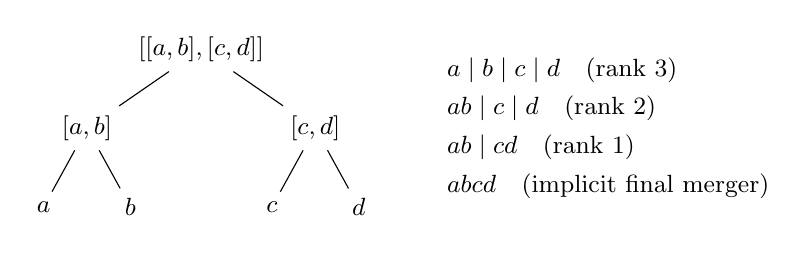
\begin{tikzpicture}[every node/.style={font=\small},level distance=12mm]
 \node (root) at (0,0) {$[[a,b],[c,d]]$};
 \node (ab) at (-1.45,-1) {$[a,b]$};
 \node (cd) at (1.45,-1) {$[c,d]$};
 \node (a) at (-2,-2) {$a$};
 \node (b) at (-.9,-2) {$b$};
 \node (c) at (.9,-2) {$c$};
 \node (d) at (2,-2) {$d$};
 \draw (root)--(ab)--(a) (ab)--(b) (root)--(cd)--(c) (cd)--(d);
 \node[align=left,anchor=west] at (3.0,-1)
 {$a\mid b\mid c\mid d$\quad(rank $3$)\\[3pt]
  $ab\mid c\mid d$\quad(rank $2$)\\[3pt]
  $ab\mid cd$\quad(rank $1$)\\[3pt]
  $abcd$\quad(implicit final merger)};
\end{tikzpicture}
\caption{A full flag of projective sign groups records binary mergers.
The left tree determines its coefficient functional.  The two children
at the root each have even parity, so interchanging them changes its
sign.  Interchanging the two leaves of either bottom pair does not.
The list is in merger order; the oriented subgroup flag has increasing
ranks $1,2,3$, with the implicit one-block merger omitted.}
\label{fig:merger-tree}
\end{figure}

The remaining task is quantitative.  Plane relations connect different
frames, so the local dimension $(h-1)!$ does not by itself give a lower
bound on the space of cycles.  We encode all these relations at once,
while retaining enough information to distinguish every supporting
subspace.

\subsection{The supporting-subspace grading and PBW}

Fix a finite ambient space $W_0$ of one of the permitted structures.
Form a commutative monoid with elements $0$, all its nonzero admissible
subspaces, and an additional element $\bot$.  For admissible subspaces
$A,B$, their sum in this monoid is the subspace $A\oplus B$ if they form
an allowed direct decomposition, and is $\bot$ otherwise.  Set
$\bot+A=\bot$, with $0$ an identity.  This operation is associative:
an iterated product avoids $\bot$ precisely when all its nonzero
subspaces form a direct decomposition, orthogonal when required.
Once directness or orthogonality fails, adjoining another summand cannot
restore it.  We call degrees other than $\bot$ \emph{good degrees}.

Let $V$ be the rational vector space with one odd generator $e_L$ for
each allowed line $L\leq W_0$, and give $e_L$ degree $L$.  Also retain
the usual word-length grading.  In the tensor algebra $T(V)$, a word
has good degree $X$ exactly when its letters are an ordered frame of
$X$; its length is then $\dim X$.  For each admissible plane $Q\leq W_0$
define
\begin{equation}\label{eq:frame-rq}
 r_Q=\sum_{(A,B):\,Q=A\oplus B}e_Ae_B
     =\sum_{\{A,B\}:\,Q=A\oplus B}[e_A,e_B].
\end{equation}
The second sum is over unordered frames and is independent of their
ordering, because the two generators are odd.  Each $r_Q$ is nonzero,
even, and homogeneous of good degree $Q$ and length $2$.

Let $\mathfrak L$ be the free Lie superalgebra on $V$, and let
\[
 P=\mathfrak L/(r_Q:Q\text{ an admissible plane})_{\Lie},\qquad
 U=T(V)/(r_Q:Q\text{ an admissible plane})_{\mathrm{ass}}.
\]
The subscripts mean the Lie ideal and the two-sided associative ideal,
respectively.  The universal properties show that $U$ is the enveloping
algebra of $P$: an associative-algebra map out of either presentation is
exactly a map on the line generators annihilating every $r_Q$.

We use the characteristic-zero super PBW theorem \cite{Scheunert1979};
the positive word-length graded form over $\Q$ is also given by
\citet[discussion following Proposition~5.2 and Theorem~5.16]{MilnorMoore1965}.
We use it
in the following explicit form.  For a homogeneous ordered basis of a Lie superalgebra,
its enveloping algebra has as a basis the ordered products of basis
elements, with each odd basis element used at most once.  Its associated
graded algebra for the number-of-factors filtration is
$\Sym(P_{\mathrm{even}})\otimes\bigwedge(P_{\mathrm{odd}})$.
The canonical map from the Lie superalgebra to its enveloping algebra
is consequently injective.  Recall why the parity qualification is
necessary: the relation for homogeneous elements is
$xy-(-1)^{|x||y|}yx=[x,y]$, and for odd $x$ it becomes
$2x^2=[x,x]$.  Ordering adjacent factors and replacing odd squares
therefore gives the stated normal forms.  The overlap of three
successive factors reduces to
\[
 [x,[y,z]]-[[x,y],z]-(-1)^{|x||y|}[y,[x,z]]=0;
\]
the overlaps with repeated odd factors are its specializations, using
$2x^2=[x,x]$ and $[x,[x,x]]=0$.  Thus these reductions are consistent
by super Jacobi.  Induction on factor length and then on the number of
out-of-order pairs gives the PBW normal forms.  This description also
shows that PBW preserves any additional grading for which the bracket
is homogeneous, including the supporting-subspace and length gradings
above.

Write $P(X)$ and $U(X)$ for the good components on a subspace $X$.
These are finite-dimensional and intrinsic to $X$.  Indeed, a product
of good degree $X$ uses only supports contained in $X$; an expression
of bad degree can never contribute to it.  Thus neither generators nor
relations supported outside $X$ affect that component.  We may
therefore form these spaces in any ambient space containing $X$.

In a good PBW monomial, the supports of its nonzero factors are
independent admissible subspaces.  In particular no basis factor can
occur twice, even when it is even.  The distinction between symmetric
and exterior multiplication changes signs but does not change the
number of such monomials.  We have proved a vector-space decomposition
in good degree:
\begin{equation}\label{eq:frame-pbw-decomposition}
 U(X)\ \cong\
 \bigoplus_{k\geq0}\ 
 \bigoplus_{X=X_1\oplus\cdots\oplus X_k\,/\,\mathfrak S_k}
 P(X_1)\otimes\cdots\otimes P(X_k),
\end{equation}
where all $X_i$ are nonzero, and the tensor factors on the right may
be ordered by any fixed order of their supports.  The term $k=0$
occurs only for $X=0$.

\begin{lemma}[Identification with coefficient assignments]
\label{lem:frame-lie-identification}
For every admissible $W$ of dimension at least two, the coefficient
construction has image of dimension $\dim P(W)$:
\[
 \dim\mathcal Z(W)=\dim P(W).
\]
\end{lemma}

\begin{proof}
The good component $T(V)(W)$ has the ordered frames as its basis.
The component of its defining ideal is spanned by all expressions
$a r_Q b$ of good degree $W$, where $a,b$ are words.  Being good forces
the outside letters and the plane $Q$ to form a direct decomposition.
Consequently their annihilator is exactly the space of functions
satisfying \eqref{eq:frame-plane-relation}.  That space is $U(W)^*$.

The good component of the free Lie superalgebra is spanned by brackets
whose letters form a frame: any other support is bad.  Its image in
$U(W)$ is $P(W)$, by PBW injectivity.  By
Lemma~\ref{lem:merger-coefficients}, the coefficient functionals of all
the full flags are precisely, up to signs and possible repetitions,
the evaluations on these brackets.  They span $P(W)$.  Restriction of
functionals $U(W)^*\to P(W)^*$ is surjective, because these spaces are
finite-dimensional.  The rank of the actual coefficient map is
therefore $\dim P(W)$, as asserted.
\end{proof}

\subsection{Normalized series and the relation kernel}

We now use formal series to count the good components in all dimensions.
Let $G_X$ be the full linear group of $X$ in the no-form case and the
full isometry group in the form cases, with $|G_0|=1$.  For any
isometry-invariant collection $M(X)$ of finite-dimensional vector
spaces, define
\[
 \mathsf M=\sum_{[X]}\frac{\dim M(X)}{|G_X|}\,[X].
\]
Here $[X]$ is a formal symbol for its isomorphism or isometry type,
and $[X][Y]=[X\oplus Y]$.  Series are completed by dimension, so each
coefficient in a product is a finite sum.  The coefficientwise order
always refers to this type basis.  If
\[
 (M*N)(W)=\bigoplus_{W=A\oplus B}M(A)\otimes N(B),
\]
then its series is $\mathsf M\mathsf N$.  To verify this, for specified
types $A,B$ the group $G_W$ acts transitively on the ordered
decompositions of these types, with stabilizer $G_A\times G_B$.
Transitivity follows by taking the direct sum of chosen isomorphisms
or isometries on the summands.  The number of decompositions is
$|G_W|/(|G_A||G_B|)$, which is exactly the normalization asserted.

Write $\mathsf P,\mathsf U$ for the series of $P,U$.  Dividing the
ordered versions of \eqref{eq:frame-pbw-decomposition} by $k!$ gives
\begin{equation}\label{eq:frame-exponential}
 \mathsf U=\exp(\mathsf P).
\end{equation}
There is no stabilizer correction beyond $k!$: the actual nonzero
summands of a direct decomposition are distinct, even if some of their
isometry types agree.  An ordering of a decomposition therefore has
exactly $k!$ possibilities.

Let $R$ be the vector space with one formal even basis element $\mathbf r_Q$
for each admissible plane $Q$, of degree $Q$.  Denote the series of
$V$ and $R$ by $v$ and $w$, respectively.  Split each relation just
before its last letter to define the left $U$-module map
\[
 d_2:U\otimes R\longrightarrow U\otimes V,
 \qquad
 d_2(u\otimes\mathbf r_Q)
   =\sum_{(A,B):Q=A\oplus B}u e_A\otimes e_B.
\]
Let $d_1:U\otimes V\to U$ be multiplication and put $C=\ker d_2$.
We have an exact sequence
\begin{equation}\label{eq:frame-relation-complex}
 0\longrightarrow C\longrightarrow U\otimes R
 \xrightarrow{d_2}U\otimes V\xrightarrow{d_1}U
 \longrightarrow\Q\longrightarrow0.
\end{equation}
Here is the only exactness assertion needing verification.  Write
$T=T(V)$ and let $I$ be the two-sided ideal generated by the $r_Q$.
Splitting the last letter identifies $T_+$ with $T\otimes V$ and
$U\otimes V$ with $T_+/(IV)$.  Hence the kernel of $d_1$ identifies
with $I/(IV)$.  Every element of $I$ is a sum of terms $a r_Q b$.
When $b$ has positive length this term lies in $IV$, by separating
the last letter of $b$.  The terms with $b=1$ are exactly the images
of $d_2$.  This proves exactness; $d_1$ plainly has image the
augmentation ideal.  These maps preserve the supporting-subspace
grading, so exactness holds in every good component.

Taking dimensions of \eqref{eq:frame-relation-complex} and normalizing
as above gives, with $\mathsf C$ the series of the good components of $C$,
\begin{equation}\label{eq:frame-euler}
 \mathsf U(1-v+w)=1+\mathsf C.
\end{equation}
This identity uses no assumption that the relations form a regular
sequence.  The possible dependencies between relations are recorded
by the actual kernel $C$.

Define the degree operator $D$ on series by $D[X]=(\dim X)[X]$.
It is a derivation because dimensions add under direct sum.  The next
inequality is the step that turns the associative presentation into
a bound on its Lie part.

The generator--relation series comparison has its classical antecedent
in \citet[Section~2, Lemmas~2--3]{GolodShafarevich1964}.
For the present coefficientwise bound, the actual kernel $C$ must
remain in the calculation. The following marked-factor argument is
what permits the later logarithmic comparison.

\begin{lemma}[Marked-factor inequality]\label{lem:frame-marked-factor}
The nonnegative series above satisfy
\begin{equation}\label{eq:frame-marked-factor}
 D\mathsf C\ \geq\ (D\mathsf P)\mathsf C
\end{equation}
coefficientwise in every isometry type.
\end{lemma}

\begin{proof}
Give $U\otimes R$ the PBW filtration on its $U$ factor and give $C$
the induced filtration.  Since $C$ is a left $U$-submodule, its
associated graded space is a submodule
\[
 \operatorname{gr} C\ \subseteq\
 \Sym_{\mathrm{super}}(P)\otimes R.
\]
The injection follows directly from using the induced filtration:
if an element of $C$ has lower filtration degree in the larger module,
it has that same lower degree in $C$.  The total dimension of a good
component is unchanged by passage to the associated graded.
This uses the induced filtration on $C$; no filteredness or strictness
of $d_2$ is required.

Fix a target space $W_0$.  Choose homogeneous bases of $P(A)$ for
every nonzero admissible $A\leq W_0$, and use the fixed labels
$\mathbf r_Q$ for the relations.  There are finitely many such basis
vectors.  Order the labels and choose one multiplicative monomial
order on all the basis vectors just chosen.  A module monomial is a
supercommutative monomial followed by a relation label.  Compare its
label first and then its monomial; ignore nonzero scalar signs.
Use the induced order in every supporting-subspace component.
Row reduction shows that the dimension of $\operatorname{gr} C(B)$
equals the number of distinct leading module monomials of its nonzero
elements.  Denote this set by $\mathcal I(B)$.

Consider a decomposition $W_0=A\oplus B$, a basis vector $p\in P(A)$,
and $m\in\mathcal I(B)$.  Choose an element with leading monomial $m$.
Every term of that element has total supporting subspace $B$.
Multiplication by $p$ therefore gives nonzero good monomials, all
distinct: no factor supported in $B$ can equal $p$, and the new
support $A$ is independent of every support in $B$.  In particular,
exterior multiplication by an odd $p$ kills none of the terms.
Multiplicativity of the monomial order implies that $pm$ is a leading
monomial in $\mathcal I(W_0)$.

Mark this appended factor $p$ and attach weight $\dim A$ to the mark.
The marked output recovers the input: $p$ determines $A$, and removing
it recovers $m$; the supports of the remaining factors together with
the relation label recover $B$.  For a fixed unmarked output, the
supports of all its factors are pairwise independent, and the relation
label itself occupies another summand of dimension two.  The sum of
the dimensions of all factors that could have been marked is thus
at most $\dim W_0$.  Counting these weighted marks gives
\[
 \sum_{W_0=A\oplus B}(\dim A)\dim P(A)\dim C(B)
   \leq (\dim W_0)\dim C(W_0).
\]
Divide by $|G_{W_0}|$ and use the transitive-decomposition count.
This is \eqref{eq:frame-marked-factor} for the type of $W_0$.
\end{proof}

We now return to the dimension bound. The remaining steps are a series
comparison and the evaluation of its constants.

Set $J=-\log(1-v+w)$, a well-defined formal series with zero constant
term.  From \eqref{eq:frame-exponential} and \eqref{eq:frame-euler},
formal differentiation gives
\[
 (1+\mathsf C)D\mathsf P=(1+\mathsf C)DJ+D\mathsf C.
\]
Subtract $\mathsf C D\mathsf P$ and apply
Lemma~\ref{lem:frame-marked-factor}.  If $DJ$ is coefficientwise
nonnegative, then
\begin{equation}\label{eq:frame-log-bound}
 D\mathsf P
 =(1+\mathsf C)DJ+
   \bigl(D\mathsf C-\mathsf C D\mathsf P\bigr)
 \ \geq\ (1+\mathsf C)DJ\ \geq\ DJ.
\end{equation}
No division by a series with unknown coefficient signs is used here.
It remains to compute $DJ$ and compare its coefficients with the
number of frames.

\subsection{Plane counts and constants}

Write $\operatorname{coeff}_{[W]}(B)$ for the coefficient of the type
$[W]$ in a series $B$.  In dimension $h$, the frame count gives
\begin{equation}\label{eq:frame-count-normalization}
 \operatorname{coeff}_{[W]}(v^h)
   =\frac{h!\,|\mathfrak F(W)|}{|G_W|}.
\end{equation}
Thus, if the degree-$h$ part of $DJ$ is at least $F_hv^h$
coefficientwise, \eqref{eq:frame-log-bound} yields
\[
 \dim P(W)\geq\frac{|G_W|}{h}\operatorname{coeff}_{[W]}(DJ)
 \geq F_h\,|\mathfrak F(W)|(h-1)!.
\]
Lemma~\ref{lem:frame-lie-identification} will then give the theorem.

First suppose that only one line type is allowed and that there is
one resulting admissible type in each dimension.  This includes the
no-form and hermitian cases.  Use a variable $t$ for the line type.
Then $v=\alpha t$, $w=\beta t^2$, where
$\alpha=|G_{\text{line}}|^{-1}$ and
$\beta=|G_{\text{plane}}|^{-1}$.  The quotient
\[
 \rho=\frac{\beta}{\alpha^2}
\]
is the reciprocal of the number of ordered allowed frames of an
admissible plane, by the decomposition count already proved.  When
$\rho\leq1/4$, set $y=(1+\sqrt{1-4\rho})/2$.  Factoring
$1-v+w=(1-yv)(1-(1-y)v)$ gives
\begin{equation}\label{eq:frame-two-roots}
 DJ=\sum_{h\geq1}\bigl(y^h+(1-y)^h\bigr)v^h.
\end{equation}
All its coefficients are positive, including the double-root case
$y=1/2$.

In a two-dimensional space over $\F_u$ without a form there are
$u+1$ possible first lines, and $u$ complementary second lines, so
there are $u(u+1)$ ordered frames.  In a hermitian plane over
$\F_{u^2}$ there are $u^2+1$ lines, of which $u+1$ are isotropic.
For completeness, in an orthonormal basis an isotropic line has a
representative $(a,1)$ with $a^{u+1}=-1$; the norm map has $u+1$
elements in each nonzero fiber.  The other $u(u-1)$ lines are
nondegenerate, each with its unique orthogonal complement.  These
are therefore the respective ordered frame counts.  For $u\geq5$
both reciprocal counts are at most $1/20$.  It follows that
$y\geq(1+\sqrt{4/5})/2>17/25$, proving the asserted uniform bound
in these two cases.

We record also the orthogonal plane count with its dependence on
determinant.  A plane with diagonal form $\operatorname{diag}(a,b)$
has
\begin{equation}\label{eq:orthogonal-plane-order}
 |G_Q|=2\bigl(u-\chi(-ab)\bigr).
\end{equation}
Indeed, the number of vectors of norm $a$ is the number of solutions
of $x^2+(b/a)y^2=1$, namely $u-\chi(-ab)$.  One way to verify this
count is to use
$\sum_{y\in\F_u}\chi(y^2-c)=-1$ for $c\ne0$.
The latter identity follows by counting $(y,z)$ with
$y^2-z^2=c$: the invertible change of variables
$(y,z)\mapsto(y-z,y+z)$ identifies these solutions with the $u-1$
pairs of nonzero elements having product $c$.
For each first vector of norm $a$, its orthogonal line has the square
class of $b$, since the determinant of the form changes by a square
under a change of basis.  There are exactly two vectors of norm $b$
on that line.  Ordered orthogonal bases with norms $(a,b)$ are acted
on freely and transitively by $G_Q$, giving
\eqref{eq:orthogonal-plane-order}.

For the same fixed norm type on both lines, $ab$ is a square and an
ordered line-frame stabilizer has order $2\cdot2=4$.  Hence the number
of ordered allowed frames is
\[
 \frac{u-\chi(-1)}2.
\]
This is at least $4$ for every odd prime power $u\geq7$: it is $4$
at $u=7$ and is at least $(u-1)/2\geq4$ for $u\geq9$.
Formula~\eqref{eq:frame-two-roots} therefore applies with
$\rho=2/(u-\chi(-1))\leq1/4$, proving the one-type assertion.

Finally allow both symmetric line types.  The determinant square
class is multiplicative under orthogonal direct sum.  Write $z$ for
the nonsquare class, with $z^2=1$, and let $t$ record dimension.
Every nondegenerate symmetric space of positive dimension over an
odd finite field is determined by its dimension and determinant
square class.  Each line has isometry group of order $2$.
Formula~\eqref{eq:orthogonal-plane-order} consequently gives
\begin{equation}\label{eq:frame-discriminant-series}
 v=\frac{1+z}{2}\,t,\qquad
 w=(a+bz)t^2,\qquad
 \{a,b\}=\left\{\frac1{2(u-1)},\frac1{2(u+1)}\right\}.
\end{equation}
Which of $a,b$ occurs at determinant square depends only on
$\chi(-1)$; the bound will be valid for either order.

Evaluation at $z=1$ gives $v=t$ and
$w=u t^2/(u^2-1)$.  Since $u/(u^2-1)<1/4$ for $u\geq5$,
the two-root computation gives
\[
 [t^h]DJ\big|_{z=1}=A_h:=x^h+(1-x)^h,
 \qquad x=\frac{1+\sqrt{1-4u/(u^2-1)}}2.
\]
At $z=-1$ we have $v=0$ and $w=\varepsilon t^2/(u^2-1)$ for
$\varepsilon\in\{1,-1\}$.  Expanding $-\log(1+w)$ therefore gives
\[
 B_h:=[t^h]DJ\big|_{z=-1}=0\quad(h\text{ odd}),
 \qquad |B_h|=2(u^2-1)^{-h/2}\quad(h\text{ even}).
\]
The two actual determinant coefficients of $[t^h]DJ$ are
$(A_h+B_h)/2$ and $(A_h-B_h)/2$.  On the other hand
$v^h=(1+z)t^h/2$ for every $h\geq1$.  Thus each determinant coefficient
of $DJ$ is at least the corresponding coefficient of $F_hv^h$, where
$F_h$ is \eqref{eq:symmetric-frame-fraction}.  In particular this
calculation keeps both types separately throughout the comparison.

We finish by proving positivity and the uniform numerical assertions.
The function $u/(u^2-1)$ decreases for $u>1$, so $x$ increases with $u$.
For each integer $h\geq1$, the function $s^h+(1-s)^h$ is nondecreasing
on $1/2\leq s\leq1$; its derivative is
$h(s^{h-1}-(1-s)^{h-1})\geq0$.  The subtracted even-degree correction
also decreases with $u$.  It suffices, therefore, to use $u=5$.
Here
\[
 x=\frac{1+1/\sqrt6}{2}>\frac7{10}.
\]
For odd $h$, $F_h\geq x^h>(17/25)^h$.  At $h=2$ a direct calculation
gives $F_2=1/2>(17/25)^2$.  For even $h\geq4$,
\[
 \frac{2\cdot24^{-h/2}}{(7/10)^h}
   =2\left(\frac{25}{294}\right)^{h/2}
   \leq2\left(\frac{25}{294}\right)^2<\frac1{50}.
\]
Consequently
\[
 F_h>\frac{49}{50}\left(\frac7{10}\right)^h
       >\left(\frac{17}{25}\right)^h.
\]
For the last inequality, divide by $(7/10)^h$ and use
$(34/35)^h\leq(34/35)^4<49/50$.
Finally
\[
 F_3=x^3+(1-x)^3
     =1-\frac{3u}{u^2-1}\geq1-\frac{15}{24}=\frac38.
\]
These inequalities also prove that every coefficient of $DJ$ used
above is nonnegative.  Applying \eqref{eq:frame-log-bound},
\eqref{eq:frame-count-normalization}, and
Lemma~\ref{lem:frame-lie-identification} proves
Theorem~\ref{thm:frame-bound} in all four cases.

\begin{remark}\label{rem:frame-cherry}
The coefficient description gives a useful relation at every bottom
pair of a merger tree.  Fix all other leaves and the surrounding
brackets.  Replacing the bracket $[e_A,e_B]$ by the sum of these
brackets over the unordered frames of the same plane gives zero in
$P$, by \eqref{eq:frame-rq}.  Every functional representing a member
of $\mathcal Z(W)$ therefore satisfies this relation on the actual
tree coefficients.  For example, when $u=5$, a plane with square
determinant has exactly one unordered frame of each homogeneous
color, and a plane with nonsquare determinant has three unordered
mixed frames.  These counts follow from
\eqref{eq:orthogonal-plane-order}: the respective group orders are
$8$ and $12$, and an ordered line-frame stabilizer has order $4$.
For a homogeneous color one divides its two ordered frames by $2$;
for a mixed frame the two possible orders have different color
patterns.  Thus the bottom-pair relation has respectively two and
three unordered terms.  This observation will allow coefficients
on specified color counts to be detected later.
\end{remark}

\section{Decorations and restriction of cycles}\label{sec:chains}

The frame construction produces cycles whose terms end at projective
sign groups. The applications require two further operations. First,
we adjoin commuting elementary generators and cancel the additional
boundary faces. Second, we pass from a group of automorphisms to a
specified subgroup while retaining a nonzero full-flag coefficient.
Both operations concern actual coefficients of simplices. In
particular, parameters describing different apartments are not counted
as independent unless their images in the chain group are independent.

The use of coefficient equations to cancel faces is shared with the
constructible and admissible cycle methods of
\citet{DiazRamos2018,DiazRamosMazza2022}. Here we state the required
injectivity separately and verify it in each group application; the
decoration counts alone do not provide it.

\subsection{Split chains and their boundary}

Write $\widetilde C_*(P)$ for the augmented rational chain complex of
a finite poset $P$, with increasing order as the orientation of every
simplex. Let $S$ and $D$ be commuting elementary abelian $p$-subgroups
of a finite group $M$, and suppose $S\cap D=1$. Given flags
\[
 u=[U_1<\cdots<U_a],\qquad
 v=[V_1<\cdots<V_b]
\]
in $S$ and $D$, respectively, put $U_0=V_0=1$. An $(a,b)$-shuffle
is a path $\gamma$ from $(0,0)$ to $(a,b)$ whose steps are $(1,0)$
or $(0,1)$. Write $(i_k,j_k)$ for its vertex after $k$ steps, and
let $\nu(\gamma)$ count pairs consisting of a $D$-step followed
later by an $S$-step. Define
\begin{equation}\label{eq:chain-split-shuffle}
 u\boxtimes v
 =\sum_{\gamma}(-1)^{\nu(\gamma)}
 [U_{i_1}V_{j_1}<\cdots<U_{i_{a+b}}V_{j_{a+b}}].
\end{equation}
Each displayed inclusion is strict, because the two factors have
trivial intersection. The origin is omitted. Empty flags are allowed:
if $a=0$ or $b=0$, there is one path and this construction is the
identity on the other flag. Extend \eqref{eq:chain-split-shuffle}
bilinearly to chains. A chain of degree $a-1$ and a chain of degree
$b-1$ give a chain of degree $a+b-1$.

This is the product shuffle of Lemma~\ref{lem:product-shuffle},
specialized to elementary groups. That lemma gives
\begin{equation}\label{eq:chain-shuffle-boundary}
 \partial(u\boxtimes v)
  =(\partial u)\boxtimes v+(-1)^a u\boxtimes(\partial v).
\end{equation}
Here and below the empty simplex has degree $-1$ and zero boundary.
Iterating the construction gives the
sum over paths with any fixed number of kinds of steps. Its sign
counts inversions between the ordered kinds, so the iteration is
associative.

Suppose that $D=D_1\times\cdots\times D_t$, where the $D_i$ are
labelled subgroups of order $p$. Its coordinate apartment, coned
at $D$, is the chain
\begin{equation}\label{eq:chain-decoration-apartment}
 a(D_1,\ldots,D_t)=
 \sum_{\pi\in\mathfrak S_t}\sgn(\pi)
 [D_{\pi(1)}<D_{\pi(1)}D_{\pi(2)}<\cdots<D].
\end{equation}
Set $a(\varnothing)=[\,]$. Interior faces cancel in pairs,
and the remaining faces give the exact formula
\begin{equation}\label{eq:chain-decoration-boundary}
 \partial a(D_1,\ldots,D_t)
 =\sum_{i=1}^t(-1)^{i-1}
    a(D_1,\ldots,\widehat D_i,\ldots,D_t).
\end{equation}
For example, when $t=2$ the boundary is $[D_2]-[D_1]$.
If $x$ is a coned apartment in $S$, then $x\boxtimes a(D_1,\ldots,D_t)$
is the apartment for the union of its basis with the decoration
basis, up to the fixed choice of orientation of $x$. More generally,
\eqref{eq:chain-split-shuffle} defines this operation on the
\emph{coefficients} of any chain $x$, without choosing an expression
of $x$ as a sum of apartments.

\subsection{The coefficient spaces to be counted}

Fix an integer $h\geq2$, and put
\[
 r=h-1,\qquad q_h=(h-1)!.
\]
A frame $\mathcal F$ with $h$ summands has a projective sign group
$S_{\mathcal F}$ of rank $r$. Denote by $V_{\mathcal F}$ the space
of actual coned frame-chain coefficients at $S_{\mathcal F}$ from
Section~\ref{sec:frames}. Thus $V_{\mathcal F}$ is a subspace of the
chain group on full flags ending at $S_{\mathcal F}$, every member
has no boundary face retaining $S_{\mathcal F}$, and
\begin{equation}\label{eq:chain-local-dimension}
 \dim V_{\mathcal F}\leq q_h.
\end{equation}
In the abstract frame model equality holds. The inequality is the
only local bound needed here.

The precise output we use from Theorem~\ref{thm:frame-bound} is the
following. For the set $\mathfrak F$ of all allowed frames of one
of the spaces specified there, it provides a subspace
\begin{equation}\label{eq:chain-frame-input}
 Z\ \subseteq\ \bigoplus_{\mathcal F\in\mathfrak F}V_{\mathcal F},
 \qquad
 \dim Z\geq F\,|\mathfrak F|q_h,
 \qquad
 \sum_{\mathcal F\in\mathfrak F}\partial x_{\mathcal F}=0
       \quad(x\in Z).
\end{equation}
The last equality uses the coarsening identifications of that
theorem. Whenever the frame model is realized by elementary
subgroups, we require these identifications to be valid subgroup
identifications. A disjoint union of compatible spaces is also
allowed, provided the same lower bound $F$ holds for every space.
The direct sum of their spaces $Z$ then satisfies the same estimate.
For example, the all-type estimates with field parameter at least
five permit $F=(17/25)^h$; for symmetric $h=3$ they permit $F=3/8$.

Equation~\eqref{eq:chain-frame-input} counts the image on coned
flag coefficients, not the dimension of the word functions that
produce it. It still retains the frame labels in the direct sum.
If different full data can give the same subgroup flag after
decorations are adjoined, their possible coincidence must be
checked separately. The next lemma states this last requirement
as an injectivity hypothesis.

\begin{lemma}[Ordinary decorations]\label{lem:decorations}
Let $M$ be a finite group, let $p$ be a prime, and let $h\geq2$ and
$t\geq0$. Consider a finite nonempty set $\mathcal X$ of data
\[
 (\mathcal F,\delta),\qquad
 \delta=(D_1,\ldots,D_t),
\]
where $S_{\mathcal F}\leq M$ is a projective sign group of rank
$r=h-1$, the labelled $D_i\leq M$ have order $p$, and
\[
 E_{\mathcal F,\delta}
   =S_{\mathcal F}\times D_1\times\cdots\times D_t
\]
is an internal direct product. Suppose the following hold.
\begin{enumerate}
\item The local coefficient space $V_{\mathcal F}$ satisfies
\eqref{eq:chain-local-dimension} and is the same whenever the same
frame occurs with different decorations. For each fixed tuple
$\delta$, its compatible frames form a set $\mathfrak F_\delta$
with a subspace $Z_\delta$ satisfying
\eqref{eq:chain-frame-input}, with a common real number $F>0$.
The boundary equality remains valid in the subgroup poset of $M$.
\item Put $\mathcal Z=\bigoplus_\delta Z_\delta$. The linear map
\begin{equation}\label{eq:chain-detection-map}
 \Phi:\mathcal Z\longrightarrow
       \widetilde C_{r+t-1}(\Ap(M)),\qquad
 \Phi(x)=\sum_{(\mathcal F,\delta)\in\mathcal X}
 x_{\mathcal F,\delta}\boxtimes a(\delta)
\end{equation}
is injective.
\item For every $i\in\{1,\ldots,t\}$, each partial datum
$(\mathcal F,D_1,\ldots,\widehat D_i,\ldots,D_t)$ that occurs
has at least $k_i>0$ completions in $\mathcal X$.
\end{enumerate}
Write $N=|\mathcal X|$. Then the image of $\Phi$ contains a space
of cycles of dimension at least
\begin{equation}\label{eq:chain-decoration-dimension}
 Nq_h\left(F-\sum_{i=1}^t\frac1{k_i}\right).
\end{equation}
In particular, if $F>\sum_i1/k_i$, there is a nonzero cycle of
degree $r+t-1$, supported on full flags ending at the rank-$r+t$
groups $E_{\mathcal F,\delta}$. At least one such full flag has
a nonzero actual coefficient. When $t=0$, the sum is zero and
there are no completion conditions.
\end{lemma}

\begin{proof}
The fixed-tuple spaces give
\[
 \dim\mathcal Z
 \geq Fq_h\sum_\delta|\mathfrak F_\delta|=FNq_h.
\]
Use \eqref{eq:chain-shuffle-boundary} on
\eqref{eq:chain-detection-map}. For fixed $\delta$, the terms
$(\partial x_{\mathcal F,\delta})\boxtimes a(\delta)$ sum to
zero by \eqref{eq:chain-frame-input}. This use of that equality is
legitimate: multiplication by subgroups of the fixed decoration
group is a well-defined operation on each common coarsening face.

It remains to cancel the terms obtained from
\eqref{eq:chain-decoration-boundary}. For each partial datum
\[
 y=(\mathcal F,D_1,\ldots,\widehat D_i,\ldots,D_t)
\]
impose the vector equation
\begin{equation}\label{eq:chain-partial-equation}
 \sum_{\substack{(\mathcal F,\delta)\in\mathcal X\\
                  \delta\text{ completes }y}}
           x_{\mathcal F,\delta}=0
       \quad\hbox{in }V_{\mathcal F}.
\end{equation}
The boundary sign $(-1)^{r+i-1}$ is common to this entire sum.
The remaining decoration apartment is also common, so
\eqref{eq:chain-partial-equation} cancels its contribution.
These equations are sufficient even if different partial data
have further coincident faces.

The following dimension count is the vector-valued analogue of the
scalar constructible-cycle count in
\citet[equation~(17), arXiv version~1]{DiazRamos2018}.
Each full datum has exactly one partial datum of kind $i$.
Since each such partial datum has at least $k_i$ completions,
there are at most $N/k_i$ of them. Each vector equation has
rank at most $q_h$ by \eqref{eq:chain-local-dimension}. Their
common kernel in $\mathcal Z$ consequently has dimension at least
\eqref{eq:chain-decoration-dimension}. Its image consists of
cycles, and injectivity of $\Phi$ preserves this dimension.
Every summand in \eqref{eq:chain-detection-map} is a full flag
of the asserted rank, so a nonzero image has the stated coefficient.
\end{proof}

Here is a useful way to check the injectivity assumption in
Lemma~\ref{lem:decorations}. Suppose a full group $E$ determines
$S_{\mathcal F}$ and its frame $\mathcal F$. Suppose also that
$D=D_1\cdots D_t$ determines the labelled axes, for instance because
they lift a fixed ordered basis of a quotient on which $D$ maps
isomorphically. Inspect a split full flag which first grows through
$D_1<D_1D_2<\cdots<D$ and then through
\[
 DU_1<\cdots<DU_r=E
\]
for a sign flag $[U_1<\cdots<U_r=S_{\mathcal F}]$.
If another datum contributes to this flag, its full group gives
the same sign group and frame. At the vertex $D$, its split form
is $U V$ with $U\leq S_{\mathcal F}$ and $V$ contained in its
decoration complement. Since $D\cap S_{\mathcal F}=1$, necessarily
$U=1$. The rank of $D$ then forces the whole alternative complement
to equal $D$. The labelled axes agree by hypothesis. The coefficient
of the inspected flag is therefore the original sign coefficient,
up to the nonzero sign of the unique shuffle taking all decoration
steps first. These flags detect every coordinate in the direct sum.
The applications will verify the recovery of $S_{\mathcal F}$,
$\mathcal F$, and the labelled axes in their particular groups.

\subsection{A rank-two decoration with three lines}

For the symplectic construction the additional elementary group is
$T\cong C_2^2$. Its three order-two subgroups are not supplied
with a preferred pair of coordinate axes. Instead we use its full
two-dimensional coefficient space
\begin{equation}\label{eq:chain-quaternion-space}
 Q_T=
 \left\{\sum_{\ell<T,\ |\ell|=2}c_\ell[\ell<T]:
             \sum_\ell c_\ell=0\right\}.
\end{equation}
For $q=\sum c_\ell[\ell<T]\in Q_T$, direct calculation gives
\begin{equation}\label{eq:chain-quaternion-boundary}
 \partial q=-\sum_\ell c_\ell[\ell].
\end{equation}
The two-dimensional space in \eqref{eq:chain-quaternion-space}
is spanned by differences of its three flags, equivalently by the
apartments from pairs of independent lines. The name in the next
lemma refers to its later realization by a projective quaternion
group; the chain statement needs only $T\cong C_2^2$.

\begin{lemma}[Quaternion decoration]\label{lem:quaternion-decoration}
Let $M$ be a finite group, $h\geq2$, $r=h-1$, and
$\varepsilon\in\{0,1\}$. Consider a finite nonempty set
$\mathcal X$ of data $(\mathcal F,T)$ if $\varepsilon=0$, or
$(\mathcal F,T,B)$ if $\varepsilon=1$, where
\[
 E=S_{\mathcal F}\times T\times B,
 \qquad \rk S_{\mathcal F}=r,\quad T\cong C_2^2,
 \quad \rk B=\varepsilon.
\]
For $\varepsilon=0$, set $B=1$ and omit it from the data.
For each fixed $(T,B)$, assume its compatible frames have a space
$Z_{T,B}$ satisfying \eqref{eq:chain-frame-input}, with a uniform
lower bound $F>0$ and local bound $q_h=(h-1)!$. Assume that the map
\begin{equation}\label{eq:chain-quaternion-detection}
 \bigoplus_{(T,B)} Z_{T,B}\otimes Q_T
 \longrightarrow \widetilde C_{r+1+\varepsilon}
                       (\mathcal A_2(M))
\end{equation}
which sends a simple tensor to the sum of the split chains
$x_{\mathcal F,T,B}\boxtimes q\boxtimes[B]$ is injective.
When $B=1$, replace $[B]$ here by the empty simplex.

For every occurring partial datum consisting of a frame, a
retained line $\ell<T$, and $B$ when present, assume there are
at least $k_T>0$ completions to full data. If $\varepsilon=1$,
assume also that every occurring $(\mathcal F,T)$ has at least
$k_B>0$ completions to a datum $(\mathcal F,T,B)$.
Then the image in \eqref{eq:chain-quaternion-detection} contains
a cycle space of dimension at least
\begin{equation}\label{eq:chain-quaternion-dimension}
 2|\mathcal X|q_h
 \left(F-\frac{3}{2k_T}-\frac{\varepsilon}{k_B}\right),
\end{equation}
where the last term is omitted if $\varepsilon=0$.
If the expression in parentheses is positive, there is a
nonzero cycle on full flags ending at groups of rank
$r+2+\varepsilon=h+1+\varepsilon$.
\end{lemma}

\begin{proof}
Put $N=|\mathcal X|$. The domain of
\eqref{eq:chain-quaternion-detection} has dimension at least
$2FNq_h$. Its sign-direction boundaries cancel for each fixed
$(T,B)$ and each coefficient in $Q_T$, by
\eqref{eq:chain-frame-input} and
\eqref{eq:chain-shuffle-boundary}.

For a retained-line partial datum $(\mathcal F,\ell,B)$, take
the coefficient $c_\ell$ in \eqref{eq:chain-quaternion-space}
from each of its completions and sum the resulting vectors in
$V_{\mathcal F}$. Impose that this sum be zero. This is a
linear condition of rank at most $q_h$. By
\eqref{eq:chain-quaternion-boundary}, these conditions cancel
all boundary terms in which the $T$-part is reduced to a line.
There are exactly $3N$ incidences between full data and their
retained-line partial data. Thus at most $3N/k_T$ such partial
data occur, costing at most $3Nq_h/k_T$ dimensions.

If $B$ is present, its boundary is the empty simplex. For each
partial datum $(\mathcal F,T)$ impose zero sum of the full
vectors in $V_{\mathcal F}\otimes Q_T$ over its $B$-completions.
Each such condition has rank at most $2q_h$, and there are at
most $N/k_B$ such data. This costs at most $2Nq_h/k_B$ further
dimensions. The common kernel therefore has dimension at least
\eqref{eq:chain-quaternion-dimension}. Its image consists of
cycles, and the assumed injectivity preserves its dimension.
The split construction shows the asserted ranks and flag lengths.
\end{proof}

The use of two parameters at $T$ is essential to this count.
There are three retained-line boundary conditions but only one
sign coefficient vector at each such partial datum. Dividing
the resulting loss by the initial factor two gives
$3/(2k_T)$. To verify the detection hypothesis, the applications
inspect split flags through $T$ and each of its three lines;
when $B$ is present they begin at $B$ and then pass through
$B\ell<BT$. These flags recover the coefficients in $Q_T$
as well as the sign-chain coefficients, once the full data
are recovered from the corresponding subgroups.

\subsection{Opposite chambers and a nonzero restricted coefficient}

We now prove the restriction statement. Its input is a homogeneous
cycle on full flags of one fixed rank. This condition will let us
take a local building cycle at a specified top group. The following
elementary building fact supplies a complement on a supported flag.

Its conclusion has the classical apartment-basis interpretation of
\citet[Theorem~1]{Solomon1969} and
\citet[Proposition~4.5 and equation~(4.6)]{Bjorner1984}: coefficients
on opposite chambers detect a top cycle. We retain a direct panel
argument, including the augmented low-rank cases, before proving the
restriction statement that uses the resulting complement.

\begin{lemma}[A supported opposite chamber]\label{lem:opposite-chamber}
Let $V$ be an $m$-dimensional vector space over $\F_p$, with
$m\geq1$, and let $\mathcal B(V)$ be its poset of proper nonzero
subspaces. Let
\[
 0=F_0<F_1<\cdots<F_m=V,\qquad \dim F_j=j,
\]
be a fixed full flag with its endpoints adjoined. Every nonzero
cycle $z\in\widetilde C_{m-2}(\mathcal B(V))$ has a supported
chamber $W_1<\cdots<W_{m-1}$ such that, on putting $W_0=0$
and $W_m=V$,
\begin{equation}\label{eq:chain-opposition}
 \dim(W_i\cap F_j)=\max\{0,i+j-m\}
       \quad(0\leq i,j\leq m).
\end{equation}
In particular, if $0<c<m$ and $F_{m-c}=K$, then
$W_c$ is a complement to $K$ in $V$.
\end{lemma}

\begin{proof}
When $m=1$, the building is empty and its unique augmented
chamber is the empty simplex; the assertion holds directly.
Suppose $m\geq2$. Write $a_W$ for the coefficient of a chamber
$W=(W_1<\cdots<W_{m-1})$ in $z$. If all its vertices except
the rank-$i$ vertex are fixed, the cycle equation is
\begin{equation}\label{eq:chain-panel}
 \sum_{W_{i-1}<X<W_{i+1},\ \dim X=i}
 a_{(W_1,\ldots,W_{i-1},X,W_{i+1},\ldots,W_{m-1})}=0.
\end{equation}
The common boundary sign $(-1)^{i-1}$ has been omitted.
For $m=2$ this is the augmentation equation at the empty
simplex. A supported completion of any such panel therefore
has another supported completion.

For a chamber $W$, set $r_{ij}=\dim(W_i\cap F_j)$. There is
a permutation $w\in\mathfrak S_m$ with
\begin{equation}\label{eq:chain-relative-permutation}
 r_{ij}=|\{k\leq i:w(k)\leq j\}|.
\end{equation}
Indeed, $r_{ij}-r_{i-1,j}$ is the dimension of the image of
$W_i\cap F_j$ in the one-dimensional space $W_i/W_{i-1}$.
As $j$ increases these images are nested, so the difference
changes from zero to one at a unique threshold $w(i)$.
Since $\sum_i(r_{ij}-r_{i-1,j})=j$, exactly $j$ thresholds
are at most $j$, proving that the thresholds form a permutation.

Choose a supported chamber maximizing the inversion number
of $w$. If $w$ is not the decreasing permutation, some
adjacent entries satisfy $a=w(i)<w(i+1)=b$. Keep its panel
fixed, and put $A=W_{i-1}$ and $C=W_{i+1}$. On the
two-dimensional quotient $C/A$ the fixed flag induces
\[
 H_j=\bigl(A+(C\cap F_j)\bigr)/A.
\]
Its dimension is $r_{i+1,j}-r_{i-1,j}$. Hence it is zero
for $j<a$, one fixed line $\ell$ for $a\leq j<b$, and
all of $C/A$ for $j\geq b$. For an intermediate subspace
$A<X<C$,
\[
 \dim(X\cap F_j)-\dim(A\cap F_j)
       =\dim\bigl((X/A)\cap H_j\bigr).
\]
Thus $X/A=\ell$ is the unique panel completion with the
two thresholds in the order $(a,b)$. Every other completion
has them in the order $(b,a)$, with all other thresholds
unchanged. Such a completion has one more inversion.
Equation~\eqref{eq:chain-panel} supplies another supported
completion, contradicting maximality. Therefore $w$ is
decreasing, and \eqref{eq:chain-relative-permutation} gives
\eqref{eq:chain-opposition}. The case $i=c$, $j=m-c$ gives
$W_c\cap K=0$, and their dimensions sum to $m$.
\end{proof}

\begin{lemma}[Restriction at a maximal index]\label{lem:restriction}
Let $M$ be a finite group, $H\leq M$, and $p$ a prime. Let
$m\geq1$ and let $\alpha\in\widetilde C_{m-1}(\Ap(M))$
be a cycle supported on full flags ending at rank-$m$
elementary abelian groups. Denote by $\mathcal E(\alpha)$
the set of top groups of flags with nonzero coefficient in
$\alpha$. Suppose that an integer $c$ satisfies
\[
 0\leq c<m,
 \qquad [E':E'\cap H]\leq p^c
      \quad(E'\in\mathcal E(\alpha)),
\]
and that a specified $E\in\mathcal E(\alpha)$ satisfies
$[E:E\cap H]=p^c$. Then there is a nonzero cycle
\[
 \beta\in\widetilde C_{m-c-1}(\Ap(H))
\]
supported on full flags of rank $m-c$, with a nonzero
coefficient at a full flag ending at $E\cap H$.
If $m-c=m_p(H)$, this cycle represents a nonzero homology class.
\end{lemma}

\begin{proof}
If $c=0$, every supported top group lies in $H$, so take
$\beta=\alpha$. Suppose henceforth $0<c<m$, and put
$K=E\cap H$.

Collect the terms of $\alpha$ ending at $E$ and delete their
last vertex. This gives a nonzero chain
$z_E\in\widetilde C_{m-2}(\mathcal B(E))$, identifying
$E$ with an $m$-dimensional $\F_p$-space. It is a cycle:
each face retaining the rank-$m$ vertex $E$ can receive a
contribution only from terms of $\alpha$ whose top is $E$.
Its coefficient equation in $\partial\alpha=0$ is exactly
the corresponding equation in $\partial z_E=0$. This includes
the augmentation equation when $m=2$.

Choose a full reference flag of $E$ through $K$, which has
dimension $m-c$. By Lemma~\ref{lem:opposite-chamber}, a full
flag with nonzero coefficient in $\alpha$ passes through a
rank-$c$ subgroup $R$ with
\begin{equation}\label{eq:chain-chosen-complement}
 E=R\times K.
\end{equation}
Fix the initial segment $\sigma=[R_1<\cdots<R_c=R]$ of
that flag, where $\rk R_i=i$.

Apply the saturated residue $R_\sigma$ of
Lemma~\ref{lem:saturated-residue}: retain the simplices whose
initial segment is $\sigma$ and delete those $c$ vertices,
with their original coefficients. The result is a chain in
the strict upper interval of $R$, and that lemma gives
\begin{equation}\label{eq:chain-restriction-residue}
 R_\sigma\partial=(-1)^c\partial R_\sigma.
\end{equation}
Its hypotheses hold because $\rk R_i=i$; no subgroup can
be inserted below $R_1$ or between consecutive vertices.
Consequently $R_\sigma\alpha$ is a cycle of degree $m-c-1$.

Every vertex $B$ in its support contains $R$ strictly and
lies in some supported top group $E'\in\mathcal E(\alpha)$.
Since $R\cap H=1$, the subgroup indices satisfy
\begin{equation}\label{eq:chain-index-sandwich}
 p^c=|R|\leq[B:B\cap H]
      \leq[E':E'\cap H]\leq p^c.
\end{equation}
All groups under consideration are subgroups of the
elementary abelian group $E'$, so these are ordinary
vector-space index inequalities. Equality throughout gives
\begin{equation}\label{eq:chain-fixed-complement-split}
 B=R\times(B\cap H).
\end{equation}
In particular $B\cap H\ne1$. Formula
\eqref{eq:chain-fixed-complement-split} holds for every
continuation vertex, with the \emph{same} fixed subgroup $R$.
It follows that
\[
 B\longmapsto B\cap H
\]
is injective on these vertices, with inverse $T\mapsto RT$
on its image. It preserves and reflects strict inclusions.

Apply this map to $R_\sigma\alpha$, and call the image
$\beta$. Since it is an injective simplicial map on the
subcomplex generated by the support, $\beta$ is a cycle and
no two distinct suffixes have been identified. The chosen
nonzero coefficient therefore survives, with its top vertex
changed from $E$ to $E\cap H$. Moreover a vertex of rank
$c+j$ becomes one of rank $j$ by
\eqref{eq:chain-fixed-complement-split}; hence every resulting
flag is full of rank $m-c$. This proves all chain assertions.
If that rank equals $m_p(H)$, there are no chains in the
next degree, so the nonzero cycle cannot be a boundary.
\end{proof}

The maximal-index hypothesis is used only in
\eqref{eq:chain-index-sandwich}. A constant index over all
supported top groups is therefore sufficient, but is not
required. Neither $m$ nor $m-c$ needs to be the maximum
elementary rank of its ambient group unless the final
top-degree conclusion is invoked. In the applications at
two, the nonzero saturated coefficient supplied by
Lemma~\ref{lem:restriction} is instead used in
Lemma~\ref{lem:propagation}.

Figure~\ref{fig:fixed-complement} illustrates the fixed-complement step
when $0<c<m$. Its middle and bottom rows are two descriptions of the
same suffix flag, which is why the intersection operation preserves
the chosen coefficient.
\begin{figure}[ht]
\centering
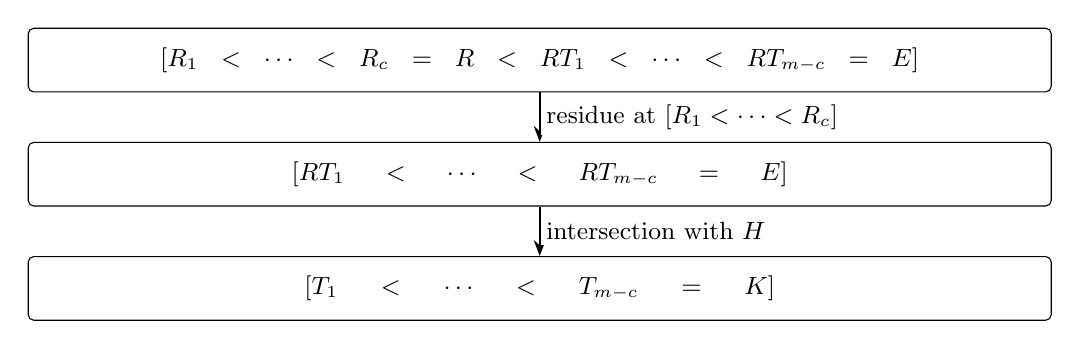
\begin{tikzpicture}[
  box/.style={draw,rounded corners=2pt,inner sep=7pt,
              text width=12.5cm,align=center,font=\small},
  transfer/.style={-{Stealth[length=2mm]},thick}]
\node[box] (full) at (0,0)
  {$[R_1<\cdots<R_c=R<RT_1<\cdots<RT_{m-c}=E]$};
\node[box] (suffix) at (0,-1.45)
  {$[RT_1<\cdots<RT_{m-c}=E]$};
\node[box] (image) at (0,-2.90)
  {$[T_1<\cdots<T_{m-c}=K]$};
\draw[transfer] (full)--node[right,font=\small,fill=white,inner sep=2pt]
  {residue at $[R_1<\cdots<R_c]$} (suffix);
\draw[transfer] (suffix)--node[right,font=\small,fill=white,inner sep=2pt]
  {intersection with $H$} (image);
\end{tikzpicture}
\caption{The chosen supported flag in Lemma~\ref{lem:restriction}, with
$E=R\times K$, $K=E\cap H$, and $0<c=\rk R<m$.
Here $T_1<\cdots<T_{m-c}=K$ is a full flag of subgroups of $K$.
The maximal-index hypothesis forces every continuation vertex $B$ in
the residue support to equal $R\times(B\cap H)$ with this same $R$.
Thus intersection with $H$ is injective on those suffix flags and
preserves the selected nonzero coefficient. The diagram depicts a
flag in that support, not an arbitrary flag in the ambient poset.
When $c=0$, the initial flag is empty, $R=1$, and the lemma uses the
original cycle in $H$.}
\label{fig:fixed-complement}
\end{figure}


\section{Linear and unitary components}\label{sec:linear}

This section applies the frame construction to linear and unitary groups.
At two we construct a coefficient to which Lemma~\ref{lem:propagation}
applies.  At odd primes we need the stronger conclusion that the coefficient
lies in the largest possible degree.  Projective commutation is the main
issue in both arguments: commuting projective transformations need not have
commuting matrix representatives.
The dimension-four cases at two are treated through their orthogonal
realizations in Propositions~\ref{prop:orthogonal} and~\ref{prop:psl45}.

\subsection{Weights, signs, and projective commutators}

We first record two elementary observations about weights.  If
$\Lambda$ is a finite subset of an affine space over $\F_p$, and translation
by a nonzero vector $a$ preserves $\Lambda$, then
\begin{equation}\label{eq:linear-translation}
 \dim\operatorname{aff}(\Lambda)\le \frac{|\Lambda|}{p}.
\end{equation}
Indeed, the translation has orbits of length $p$.  If there are $t$ orbits,
choose representatives $\lambda_1,\ldots,\lambda_t$; the affine span is
generated by $a$ and the $t-1$ differences $\lambda_i-\lambda_1$.

For the second observation, let an elementary abelian $p$-group $D$ act
faithfully projectively on a vector space in characteristic different from
$p$.  Suppose that its matrix representatives commute.  Over an algebraic
closure, rescale representatives of a basis of $D$ to have order $p$.
They give a linear representation of $D$ with a set of characters
$\Lambda\subseteq D^*$.  The differences of these characters span $D^*$:
an element annihilated by every difference acts by a scalar and is therefore
trivial in $D$.  Thus
\begin{equation}\label{eq:linear-affine-rank}
 \dim\operatorname{aff}(\Lambda)=\rk D.
\end{equation}
A transformation centralizing the projective action, and acting trivially
on the $p$th roots of unity, permutes these characters by a common
translation.  To see this, conjugating each chosen representative changes
it by a scalar; the scalars, which are $p$th roots of unity after
normalization, form a character of $D$.

Here is the complementary estimate when the representatives do not commute.
It will also be useful in the exceptional case of Section~\ref{sec:exceptional}.

\begin{lemma}\label{lem:projective-rank}
Let $D$ be an elementary abelian $p$-subgroup of $\PGL(V)$, where
$\dim V=n$ and the characteristic of the field is different from $p$.
The scalar commutators of representatives define an alternating bilinear
pairing on $D$ with values in the $p$th roots of unity.  If this pairing
has rank $2a$, then
\[
 p^a\mid n,
 \qquad
 \rk D\le 2a+\frac{n}{p^a}-1.
\]
In particular, for odd $p$, $n\ge5$, and $a>0$,
\begin{equation}\label{eq:odd-pairing-strict}
 \rk D<n-2.
\end{equation}
\end{lemma}

\begin{proof}
We may extend the field to its algebraic closure.  If $X,Y$ represent
elements of $D$, then $[X,Y]$ is scalar, and $X^p$ is scalar.  Consequently
$[X,Y]^p=[X^p,Y]=1$.  The commutator identities for central commutators
give the asserted alternating bilinear pairing.

Let $R$ be its radical.  Choose representatives of generators of $R$ and
rescale them to order $p$.  They commute with all the representatives in
question.  Let $t$ be the number of their distinct simultaneous weights.
Their weight ratios separate $R$ projectively, so $\rk R\le t-1$.
Choose a symplectic basis $x_1,y_1,\ldots,x_a,y_a$ for a complement of $R$
in $D$, with representatives normalized to order $p$.  On each radical
weight space, the commuting $x_i$ have simultaneous eigenspaces.
The $y_i$ translate their $a$ eigenvalue coordinates independently through
all $p$ possibilities.  They therefore permute these eigenspaces freely
in orbits of size $p^a$, with equal dimensions within an orbit.
Every radical weight space has positive dimension divisible by $p^a$.
It follows that $p^a\mid n$, $t\le n/p^a$, and
$\rk D=2a+\rk R\le 2a+n/p^a-1$.

For the final assertion put $u=p^a$.  Except when $(p,a)=(3,1)$,
we have $u>2a+2$: for $a=1$ this follows from $p\ge5$, and for $a\ge2$
it follows from $3^a>2a+2$.  Since $n\ge u$,
\[
 n-2-\left(2a+\frac n u-1\right)
 =n\left(1-\frac1u\right)-2a-1
 \ge u-2a-2>0.
\]
In the remaining case $3\mid n$ and $n\ge5$, so $n\ge6$, and the
same difference is $2n/3-3\ge1$.
\end{proof}

Let $L=\PSL_n(q)$ or $\PSU_n(q)$, and put $M=\PGL_n(q)$ or
$\PGU_n(q)$, respectively.  In the unitary notation, $\GU_n(q)$ denotes
the group of isometries of a nondegenerate hermitian form over
$\F_{q^2}$; its projective image also contains every projective
similitude, since the norm map onto $\F_q^\times$ is surjective.
In the linear case set $C=\F_q^\times$, and in the unitary case set
$C=\mu_{q+1}\subseteq\F_{q^2}^\times$.  Determinant induces
\begin{equation}\label{eq:linear-determinant}
 M/L\cong C/C^n.
\end{equation}
In particular this quotient is cyclic.

A line frame $\mathcal D$ is an unordered direct-sum decomposition into
$n$ lines; in the unitary case the lines are required to be orthogonal
and nondegenerate.  For a prime $p\mid |C|$, define $S(\mathcal D)$ to
be the projective images of the diagonal operators with entries in
$\mu_p$.  Thus $S(\mathcal D)\cong\F_p^n/\langle(1,\ldots,1)\rangle$
has rank $n-1$.  For any fixed $L\le H\le\Aut(L)$,
\begin{equation}\label{eq:linear-hzero}
 h_0:=\rk(S(\mathcal D)\cap H)\in\{n-2,n-1\}
\end{equation}
is independent of $\mathcal D$.  Indeed all these frames are conjugate
under $M$, and their images in the abelian group $M/L$ are consequently
the same subgroup, of order at most $p$.

We use the standard automorphism description for these groups in
dimension $n\ge5$; see \citet[Section~2 and statements~3.2--3.6]{Steinberg1960}
and \citet{GLS1998}.  If $q=r^f$, the quotient
$\Aut(\PSL_n(q))/\PGL_n(q)$ is the product of the field group of order
$f$ and the diagram group of order two.  The diagram operation is
$\gamma:g\mapsto(g^{-1})^{\mathsf t}$.  The quotient
$\Aut(\PSU_n(q))/\PGU_n(q)$ is the cyclic field group of order $2f$
on $\F_{q^2}$.  Semilinear isometries represent the latter automorphisms.
Thus an elementary subgroup has at most two external directions at two
in the linear case, at most one in the unitary case, and at most one
at odd primes in either case.

A \emph{correlation} here is a linear or semilinear identification
with the dual space, acting on the group through inverse transpose.
A dual frame consists of the lines of linear functionals vanishing
on all but one summand of the original frame.
A frame is matched with its dual frame when each of its lines is
matched with the corresponding dual line under this identification.

\begin{lemma}\label{lem:linear-sign-centralizer}
Suppose $q$ is odd and $n\ge5$.  Set
$S=S(\mathcal D)$ and $S_L=S\cap L$ for a line frame as above, using
$p=2$.  Every automorphism centralizing $S_L$ preserves each line of
$\mathcal D$, or matches it with the corresponding line of the dual
frame when it is a correlation.  It centralizes $S$.  Every involution
in $M$ centralizing $S_L$ belongs to $S$.
\end{lemma}

\begin{proof}
The preimage of $S_L$ in $\F_2^n$ is either all of $\F_2^n$ or
the kernel of the total-parity functional.  This follows directly from
the determinant formula; when $n$ is odd the second possibility cannot
occur, since the simultaneous sign belongs to that preimage.
For $n\ge5$, the coordinate characters on this preimage are distinct:
a relation equating two coordinates is neither the zero relation nor
the total-parity relation.  Their differences factor through $S_L$ and
span its dual.  After choosing a normalization, the corresponding $n$
weights therefore have affine rank $\rk S_L\ge n-2$.

Field operations and inverse-transpose leave binary sign values unchanged.
Projective centralization can consequently permute the weights only by a
common translation.  A nonzero translation would give affine rank at most
$n/2$ by \eqref{eq:linear-translation}, contrary to $n-2>n/2$.
Every weight line is therefore preserved individually, with the indicated
dual interpretation for a correlation.  Each such operation centralizes
all binary diagonal signs.  Finally a line-preserving projective
involution in $M$ has diagonal entries whose ratios square to one;
after removing a common scalar these entries are all $1$ or $-1$.
It belongs to $S$.
\end{proof}

\subsection{Compatible frames for involutory decorations}
\label{subsec:linear-compatible}

We next identify the frame spaces to which Theorem~\ref{thm:frame-bound}
will be applied.  A decoration is an involution outside $M$.  A frame is
compatible with it if every line is stable, with matching to the dual
frame in the correlation case.  For several decorations we require them
to commute and require compatibility with each of them.  In what follows
we consider only tuples having at least one compatible frame.

We use the following fixed-vector form of Galois descent. Let $K/k$
be a cyclic finite-field extension of degree $d$, with generator
$\sigma$, and let $B$ be an additive map on a finite-dimensional
$K$-space $V$ satisfying $B(av)=\sigma(a)B(v)$ and $B^d=\id$.
The powers of $B$ define a semilinear Galois action, and
\citet[Proposition~5.5]{MilneDescent2024} gives
\[
 K\otimes_k V^B\longrightarrow V,\qquad a\otimes v\longmapsto av,
\]
as an isomorphism. In particular $\dim_k V^B=\dim_K V$.
Every $B$-stable $K$-subspace descends by the same assertion applied
to its restriction; see also \citet[Proposition~3.5]{MilneDescent2024}.
Thus a stable line has a fixed nonzero generator.

After a form $f$ has been made $\sigma$-equivariant, meaning
$f(Bv,Bw)=\sigma(f(v,w))$, its Gram matrix in a fixed-vector basis
has entries in $k$. Its restriction consequently
extends back to the original form and preserves nondegeneracy.
For a hermitian form with field involution $\tau$ commuting with
$\sigma$, the restricted form has involution $\tau|_k$; it is
symmetric when that restriction is the identity. All field
involutions used here commute. The normalizations giving $B^d=\id$
and equivariance of the form are checked separately below; scalar
Hilbert~90, as in \citet[Corollary~5.25]{MilneFields2022}, handles
only the scalar part of those checks.

In the linear case, an external field involution requires $q=s^2$;
write $\sigma:x\mapsto x^s$.  On a compatible frame a representative
is $T=\diag(a_1,\ldots,a_n)\sigma$, and $T^2=cI$ implies
$a_i a_i^\sigma=c$ for every $i$.  Multiplying $T$ by $a_1^{-1}$ makes
$T^2=I$.  Semilinear descent gives an $n$-dimensional fixed space
$V_0$ over $\F_s$, with $V=V_0\otimes_{\F_s}\F_q$.
A stable line has a fixed generator by the one-dimensional norm-one
equation, so compatible frames correspond exactly to line frames of
$V_0$.

A correlation without field action is represented by a nonsingular
bilinear form.  The involutory condition says that its transpose is a
scalar multiple of itself.  In coordinates from a compatible frame its
matrix is diagonal and nonsingular; the scalar is therefore one.
The form is symmetric, and the compatible frames are its orthogonal
nondegenerate line frames.  For a diagram-field involution, the same
argument uses a $\sigma$-sesquilinear form.  Its conjugate transpose is
a scalar multiple of itself; scaling the form, using the norm-one scalar
equation, makes it hermitian.  Its compatible frames are hermitian frames
with parameter $s$.  Alternating forms have no compatible nondegenerate
line frame and do not occur in either assertion.

If there are two independent external involutions, choose their external
basis to be field and diagram-field.  Descend the first one to $\sigma$.
Choose generators for the lines of one compatible frame in the descended
space.  In these coordinates write the other involution as
$\operatorname{Int}(D)\gamma\sigma$, where $D$ is nonsingular diagonal
and $\operatorname{Int}(D)(g)=DgD^{-1}$.  Projective
commutation with $\sigma$ gives $D^\sigma=cD$.  Dividing by any diagonal
entry makes every entry of $D$ lie in $\F_s$.  The corresponding
correlation form on $V_0$ has Gram matrix $D^{-1}$.  Indeed, for
$g\in\GL(V_0)$ and $\lambda\in\F_s^\times$,
\[
 gDg^{\mathsf T}=\lambda D
 \quad\Longleftrightarrow\quad
 g^{\mathsf T}D^{-1}g=\lambda D^{-1}.
\]
This form is symmetric and nondegenerate over $\F_s$.
A frame is compatible with both
involutions precisely when it is the scalar extension of an orthogonal
frame for this symmetric form: the first condition descends its lines,
and the second is orthogonality for that form.

In the unitary case the unique external involution induces
$\tau:x\mapsto x^q$ on $\F_{q^2}$.  Take an orthonormal basis along a
compatible frame.  A unitary semilinear representative has the form
\[
 T=\diag(t_1,\ldots,t_n)\tau,
 \qquad t_i^{q+1}=1.
\]
It follows that $T^2=I$.  This conclusion uses compatibility with a
\emph{nondegenerate orthogonal} frame.  An arbitrary projective unitary
semilinear involution can instead have square $-I$, which cannot be
removed by multiplying by a norm-one scalar.  No such involution is
included here.  The fixed space of $T$ has dimension $n$ over $\F_q$.
The original hermitian form restricts to a nondegenerate symmetric form
on this space: its values on fixed vectors are fixed by $\tau$, and
hermitian symmetry then becomes ordinary symmetry.  Compatible unitary
frames correspond exactly to orthogonal nondegenerate line frames in
this fixed space.

These descriptions also identify all coarsenings of frames.  A sum of
lines descends to the corresponding sum of fixed lines, and the subgroup
requiring equal signs on that sum is unchanged by the description.
Adjoining the fixed decorations preserves these identifications.  Thus
the frame relations in Theorem~\ref{thm:frame-bound} are actual subgroup
face relations for the decorated groups.

\subsection{The construction at two}

\begin{proposition}\label{prop:linear-two}
Let $G$ have least order among finite groups with $O_2(G)=1$ and
$\widetilde H_*(\mathcal A_2(G);\Q)=0$.
Then $G$ has no simple component isomorphic to $\PSL_n(q)$ or
$\PSU_n(q)$ with $n\ge5$ and $q$ of characteristic at least five.
\end{proposition}

\begin{proof}
Suppose $L$ is such a component.  Consider all elementary abelian
$2$-subgroups $A\le N_G(L)$ for which $LA$ acts faithfully on $L$,
$O_2(C_G(LA))=1$, and $A\cap L$ contains $S(\mathcal D)\cap L$
for some line frame $\mathcal D$.  This family is nonempty: take
$A=S(\mathcal D)\cap L$ and use Lemma~\ref{lem:component-core}.
It is closed under elementary overgroups that are faithful
configurations, since each such overgroup still contains the same
subgroup $S(\mathcal D)\cap L$.
Choose a member of maximum rank, put $H=LA$, and identify $H$ with its
faithful image in $\Aut(L)$.

For its frame put $S=S(\mathcal D)$.  Lemma~\ref{lem:linear-sign-centralizer}
shows that $A$ centralizes $S$ and $A\cap M\le S$.  Adjoining $S\cap H$
would give another member of the same family with the same generated
group $H$, so maximality implies
\[
 A\cap M=S\cap H.
\]
Let $J_0$ be the image of $A$ in $\Aut(L)/M$ and write $d=\rk J_0$.
Choose a fixed basis $j_1,\ldots,j_d$ of $J_0$, and choose its lifts
$b_1,\ldots,b_d$ in a complement $T$ to $A\cap M$ in $A$.
For $d=2$ use the field and diagram-field basis above.  These lifts are
commuting involutions compatible with $\mathcal D$.  Filling out the
signs gives
\begin{equation}\label{eq:linear-E-intersection}
 E=S\times T,
 \qquad \rk E=n-1+d,
 \qquad E\cap H=A.
\end{equation}

For the construction, vary the frame and the ordered decorations subject
to the following requirements: $b_i\in H$ maps to $j_i$, the $b_i$ are
commuting involutions, and the frame is compatible with all of them.
The original data show that this set is nonempty.  All the resulting
groups $E$ have rank $n-1+d$.  They also have the same intersection index
in $H$, and every intersection generates $H$ over $L$.
Here is the verification of the latter point.  The image
$B$ of $S(\mathcal D)$ in $M/L$ is independent of the frame.
For the original $A$, its subgroup $A\cap M$ maps onto
$(H\cap M)/L$, since $A$ maps onto $H/L$.  Therefore $B$ contains
$(H\cap M)/L$.  For every new frame, $S(\mathcal D)\cap H$ maps onto
that same subgroup.  Together with the $b_i$ it consequently generates
$H/L$.  If $h_0$ is as in \eqref{eq:linear-hzero}, then for every datum
\begin{equation}\label{eq:linear-constant-index}
\begin{gathered}
 A'=E\cap H=(S(\mathcal D)\cap H)\times T,
 \qquad LA'=H,\\
 \rk A'=h_0+d,\qquad |E:A'|=2^c,\qquad
 c=n-1-h_0\in\{0,1\}.
\end{gathered}
\end{equation}

For each fixed decoration tuple, the preceding descent gives all the
frames of a linear, symmetric, or hermitian space of dimension $n$.
Its field parameter is $q$ or a subfield parameter $s$, and in every
case is at least five.  In the symmetric cases all line norm types are
allowed; the estimate is uniform over the isometry types that arise.
By Theorem~\ref{thm:frame-bound}, its space of
frame assignments has dimension at least the fraction
\[
 F=\left(\frac{17}{25}\right)^n
\]
of the number of compatible frames times $(n-1)!$.
We now count completions after one decoration has been omitted.

Fix a frame and one existing completion.  Multiplying the omitted
decoration by a diagonal element $X$ preserves compatibility.  The
following cyclic choices for each entry of $X$ also preserve its order
and its commutation with all retained decorations:
\[
\begin{array}{c|c|c}
\text{omitted direction}&\text{condition on an entry }x&k\\
\hline
\text{linear diagram}&x\in\F_q^\times&q-1\\
\text{linear field},\ q=s^2&x^{s+1}=1&s+1\\
\text{linear diagram-field},\ q=s^2&x\in\F_s^\times&s-1\\
\text{unitary external involution}&x^{q+1}=1&q+1
\end{array}
\]
In the two-direction case the last two linear prescriptions apply.
Indeed the field direction acts on diagonal entries by $x\mapsto x^s$,
and the diagram-field direction by $x\mapsto x^{-s}$.  Thus a norm-one
modification of the field lift is fixed by the retained diagram-field
lift, whereas a fixed-field modification of the diagram-field lift is
fixed by the retained field lift.  The same formulas show that the
square of the modified lift remains projectively trivial.  They apply
even when the original matrix representatives commute only projectively.

There are $k^n$ diagonal choices and $k^{n-1}$ projective choices.
We keep those projective modifications that lie in $L$; this ensures
that the new decoration remains in $H$ with the required external image.
The determinant homomorphism from the modification group to the cyclic
group $M/L$ has image of exponent dividing $k$, hence order at most $k$.
There are therefore at least $k^{n-2}$ permitted modifications.
Distinct projective modifications give distinct decorations.  Since
$k\ge4$, every partial datum has at least $4^{n-2}$ completions.
The inequality required in Lemma~\ref{lem:decorations} follows from
\begin{equation}\label{eq:linear-completion-inequality}
 \left(\frac{17}{25}\right)^n>\frac{2}{4^{n-2}}
 \qquad(n\ge5).
\end{equation}
At $n=5$ the left side exceeds $(2/3)^5=32/243>1/32$, which is the
right side; increasing $n$ multiplies their ratio by $68/25>1$.
For $d=0$ there are no decoration equations, and for $d=1$ the right
side can of course be halved.

It remains to verify that the assignments counted here are detected by
actual full-flag coefficients, as required by Lemma~\ref{lem:decorations}.
The top group $E$ recovers its full signs as $E\cap M$.
The simultaneous eigenspaces of these signs recover the frame.
For fixed $E$ and frame, take split flags through the full decoration
span $T$ and then through the sign flag.  If a second decoration span
$T'$ contributes to such a split flag, the vertex $T$ must split with
respect to $S\oplus T'$.  Its projection onto $J_0$ is an isomorphism
and its rank is $d$.  Hence its sign part is zero and $T=T'$.
The fixed basis $j_1,\ldots,j_d$ then recovers the individual $b_i$.
The coefficients above this vertex are precisely the original sign
coefficients, up to the fixed shuffle signs.  Thus these flags detect
all the counted parameters.  When $d=0$, detection is the undecorated
assertion of Theorem~\ref{thm:frame-bound}.

Lemma~\ref{lem:decorations} now supplies a nonzero homogeneous cycle
on full flags with top rank $n-1+d$ in the ambient automorphism group.
By \eqref{eq:linear-constant-index}, Lemma~\ref{lem:restriction} applies
at any supported top group: $c\le1<n-1+d$.  It produces a cycle in
$\mathcal A_2(H)$ with a nonzero coefficient on a saturated flag ending
at $A'=E\cap H$, of rank $h_0+d$.

We finally apply Corollary~\ref{cor:maximal-family} at this actual
coefficient.  The subgroup
$A'$ contains $S(\mathcal D)\cap L$, has the original maximum rank,
and satisfies $LA'=H$; thus $O_2(C_G(LA'))=O_2(C_G(H))=1$.
It therefore belongs to the family that was maximized.  The corollary
uses the nonzero saturated coefficient just constructed to give
$\widetilde H_*(\mathcal A_2(G);\Q)\ne0$, the desired contradiction.
\end{proof}

\subsection{Odd-prime unitary extensions}

\begin{proposition}\label{prop:unitary-odd}
Let $p$ be an odd prime, let $q$ be odd with $p\mid q+1$, and let
$L=\PSU_n(q)$ with $n\ge5$.  If $L\le H\le\Aut(L)$ and $H/L$ is
elementary abelian of $p$-power order, then
\[
 \widetilde H_{m_p(H)-1}(\Ap(H);\Q)\ne0.
\]
Here $m_p(H)$ denotes the maximum rank of an elementary abelian
$p$-subgroup of $H$.
\end{proposition}

\begin{proof}
Put $K=\F_{q^2}$ and $M=\PGU_n(q)$, and use the $p$-sign group of
an orthogonal line frame.  Its intersection with $H$ has the constant
rank $h_0\in\{n-2,n-1\}$ of \eqref{eq:linear-hzero}.
We first prove that
\begin{equation}\label{eq:unitary-rank-dichotomy}
 m_p(H)\in\{h_0,h_0+1\},
\end{equation}
and that in the second case the larger rank is attained by
$(S(\mathcal D)\cap H)\times\langle b\rangle$, where $b$ is a
field decoration preserving each line of $\mathcal D$.

Let $B\le H$ be elementary with $\rk B>h_0$, and set $D=B\cap M$.
There is at most one external direction, so $\rk D\ge n-2$.
By Lemma~\ref{lem:projective-rank}, the scalar commutator pairing of
$D$ is zero.  Choose commuting unitary representatives $U_1,\ldots,U_r$
of a basis of $D$, where $r=\rk D$, and write $U_i^p=c_iI$.
Over an algebraic closure choose $t_i^p=c_i$ and put $X_i=t_i^{-1}U_i$.
Fix a primitive $p$th root $\zeta$.  The simultaneous weights of the
$X_i$ form a set $\Lambda\subseteq\F_p^r$ with
$\dim\operatorname{aff}(\Lambda)=r$ and $|\Lambda|\le n$; the actual
eigenvalue of $U_i$ at $\lambda$ is $t_i\zeta^{\lambda_i}$.

Unitarity identifies this representation with its conjugate dual, so
the multiset of joint eigenvalues is preserved by raising every entry
to the power $-q$.  Since $-q\equiv1\pmod p$, this operation acts on
$\Lambda$ by the common translation $\lambda\mapsto\lambda+\delta$,
where
\[
 \zeta^{\delta_i}=t_i^{-(q+1)}.
\]
The right side is a $p$th root of unity because $c_i^{q+1}=1$.
A nonzero translation would imply
\[
 \rk D\le |\Lambda|/p\le n/p<n-2,
\]
by \eqref{eq:linear-translation}, which is impossible.  The translation
is therefore zero.  Hence $t_i^{q+1}=1$ for every $i$.  In particular
$t_i\in\mu_{q+1}\subseteq K$, so the $X_i$ are unitary matrices over
$K$ with eigenvalues in $\mu_p$.  Their simultaneous eigenspaces are
defined over $K$.  Distinct weights are orthogonal: if their $i$th
eigenvalues differ, invariance of the hermitian form multiplies their
pairing by the nonidentity ratio of those eigenvalues.  Each eigenspace
is nondegenerate since their orthogonal direct sum is the whole space.
They therefore admit orthogonal nondegenerate line refinements over $K$.
On such a refinement the $X_i$ are diagonal $p$-signs, so their
projective images belong to $S(\mathcal D)$.
Thus $D\le S(\mathcal D)\cap H$ for some frame.

If $B=D$, this contradicts $\rk B>h_0$.  Otherwise choose
$b\in B\setminus M$.  Its field action has order $p$ and hence fixes
the cyclic group $\mu_p$, whose automorphism group has order $p-1$.
Projective commutation with $D$ once more permutes its weights by a
translation.  The same rank inequality excludes a nonzero translation,
so $b$ preserves every nondegenerate eigenspace just obtained.

Write $q=s^p$ and let $\sigma$ be the order-$p$ field action of $b$
on $K$; its fixed field is $K_0=\F_{s^2}$.  A unitary semilinear
representative $T$ of $b$ satisfies $T^p=cI$, where
$c\in\mu_{q+1}$ and $c^\sigma=c$, so $c\in\mu_{s+1}$.
The norm
\begin{equation}\label{eq:unitary-norm}
 N:\mu_{q+1}\longrightarrow\mu_{s+1}
\end{equation}
for $K/K_0$ is onto.  Indeed, writing
\[
 k=\frac{s^p+1}{s+1},\qquad
 \ell=\frac{s^p-1}{s-1},
\]
its exponent is $(s^{2p}-1)/(s^2-1)=k\ell$.
Since $p$ is odd, $\ell=1+s+\cdots+s^{p-1}\equiv1\pmod{s+1}$.
As $|\mu_{q+1}|=k(s+1)$, the image has order $s+1$ and the kernel
has order $k$.  This norm is unchanged if another generator of
$\Gal(K/K_0)$ is used.  Choose $a\in\mu_{q+1}$ with $N(a)=c^{-1}$.
Replacing $T$ by $aT$ gives $T^p=I$ while preserving its unitary
semilinear action.

Semilinear descent now gives an $n$-dimensional space $V_0$ over $K_0$.
The hermitian form descends: on fixed vectors its values lie in $K_0$,
and the involution $x\mapsto x^q$ restricts there to $x\mapsto x^s$.
Each of the $T$-stable nondegenerate eigenspaces descends as well.
Choose an orthogonal line frame within each descended eigenspace and
extend scalars back to $K$.  The resulting frame $\mathcal D$ is
compatible with $b$, contains $D$ in its signs, and has each line fixed
by $b$.  Since $\sigma$ fixes $\mu_p$, $b$ centralizes all of
$S(\mathcal D)$.  Hence
\[
 B\le (S(\mathcal D)\cap H)\times\langle b\rangle,
\]
an elementary group of rank $h_0+1$.  This proves
\eqref{eq:unitary-rank-dichotomy} with the asserted compatible realization.

We now construct a cycle in the degree dictated by this calculation.
Set $c=n-1-h_0\in\{0,1\}$.  If $m_p(H)=h_0$, use
Theorem~\ref{thm:frame-bound} on all unitary frames with parameter $q$.
Here $q\ge5$: the smaller odd possibility $q=3$ has no odd prime
dividing $q+1$.  It gives a nonzero cycle with top rank $n-1$ in
$M$.  Its intersection index in $H$ is the constant $p^c$, so
Lemma~\ref{lem:restriction} produces a nonzero cycle in degree
\begin{equation}\label{eq:unitary-undecorated-degree}
 (n-1)-1-c=h_0-1=m_p(H)-1.
\end{equation}

Suppose instead that $m_p(H)=h_0+1$.  Fix the nontrivial field image
of a compatible element $b$ supplied above.  Use all pairs consisting
of an order-$p$ lift of this fixed image in $H$ and a compatible
orthogonal line frame.  For each lift that occurs, the normalization and
descent just proved identify its compatible frames with all hermitian
frames over the parameter $s=q^{1/p}$.  Fermat's congruence gives
$s\equiv s^p=q\equiv-1\pmod p$, so $p\mid s+1$.
As $s$ is odd, it follows that $s\ge5$.  The frame fraction is again
at least $(17/25)^n$.

At a fixed frame vary a given lift by a diagonal matrix with all entries
in the kernel of \eqref{eq:unitary-norm}.  The kernel has order
$k=(q+1)/(s+1)$, and the norm equation ensures that the modified lift
still has projective order $p$.  There are $k^{n-1}$ choices modulo
common scalars.  As in the determinant calculation at two, restricting
the modification to $L$ loses a factor at most $k$, leaving at least
$k^{n-2}$ completions in $H$.  To bound $k$, write $p=2a+1$ and note
\[
 k=1+\sum_{j=1}^{a}(s^{2j}-s^{2j-1})
 \ge s^2-s+1\ge21.
\]
Consequently
\[
 \left(\frac{17}{25}\right)^n>\frac1{21^{n-2}}
 \qquad(n\ge5).
\]
At $n=5$ the left side exceeds $1/32>1/9261$, and increasing $n$
multiplies the ratio of the two sides by $357/25$.
The detection argument used above applies without change: the full
group $E=S(\mathcal D)\times\langle b\rangle$ recovers its linear
kernel and frame, and the split flags through the line $\langle b\rangle$
recover the lift of the fixed field generator.  All the hypotheses of
Lemma~\ref{lem:decorations} are therefore satisfied.

We obtain a nonzero cycle with top rank $n$.  For every supporting group
$E$, the decoration lies in $H$ and
\[
 E\cap H=(S(\mathcal D)\cap H)\times\langle b\rangle,
 \qquad |E:E\cap H|=p^c.
\]
Lemma~\ref{lem:restriction} gives a nonzero cycle of degree
\begin{equation}\label{eq:unitary-decorated-degree}
 n-1-c=h_0=m_p(H)-1.
\end{equation}
In both cases the resulting cycle has a nonzero coefficient and lies
in the largest possible chain degree of $\Ap(H)$.  There are no chains
one degree higher, so this cycle cannot be a boundary.  This proves the
proposition.
\end{proof}

\section{Symplectic components at two}\label{sec:symplectic}

For a symplectic component, signs on a decomposition into planes leave
room for a quaternion four-group.  Its two-dimensional space of local
chain coefficients provides the extra factor needed in the smallest
case.  We construct the cycle directly inside the selected faithful
component extension, then apply Lemma~\ref{lem:propagation} at a
supported full flag.

\begin{proposition}\label{prop:symplectic}
A minimal-order counterexample to \eqref{eq:HQC} at $p=2$ cannot have a
simple component isomorphic to $\PSp_{2n}(q)$, where $n\geq3$ and $q$
has characteristic at least five.
\end{proposition}

Throughout this section, $V$ is a $2n$-dimensional vector space over
$\F_q$ with nondegenerate alternating form $\omega$, and
$L=\PSp(V)$.  Write $M=\PGSp(V)$ for the projective group of linear
symplectic similitudes.  In this range the automorphism theorem
\citep[Section~2 and statements~3.2--3.6]{Steinberg1960} gives
$\Aut(L)=M\rtimes\Gal(\F_q/\F_\ell)$, where $\ell$ is the
characteristic; there is no additional diagram automorphism.  Thus
$\Aut(L)/M$ is cyclic.  We use projective classes of semilinear
similitudes for the elements of this group, as in
Section~\ref{sec:reductions}.

\subsection{Plane signs and the quaternion action}

Let $\mathcal D=\{V_1,\ldots,V_n\}$ be an unordered orthogonal
decomposition of $V$ into nondegenerate planes.  Its linear sign group
and projective sign group are
\[
\widehat S(\mathcal D)
 =\{\diag(\epsilon_1\id_{V_1},\ldots,
                   \epsilon_n\id_{V_n}):\epsilon_i\in\{1,-1\}\},
\qquad
S(\mathcal D)=\widehat S(\mathcal D)/\langle-\id_V\rangle.
\]
All these signs are symplectic, and $S(\mathcal D)\leq L$ has rank
$n-1$.

A \emph{quaternion four-group compatible with $\mathcal D$} is a
subgroup $T\leq L$ generated by the projective classes of two
operators $I,J\in\Sp(V)$ such that
\begin{equation}\label{eq:symp-quaternion}
I^2=J^2=-\id_V,\qquad IJ=-JI,
\end{equation}
and both operators preserve every $V_i$.  On each plane these
operators generate its full matrix algebra.  Indeed, after extending
scalars to an algebraic closure, $I$ has two distinct eigenvalues and
$J$ interchanges the two eigenlines.  The resulting diagonal and
off-diagonal matrix units span the full matrix algebra; its dimension
is therefore already four over $\F_q$.

Such pairs exist over every finite field of odd order.  On a plane
choose
\[
I=\begin{pmatrix}0&1\\-1&0\end{pmatrix},\qquad
J=\begin{pmatrix}a&b\\b&-a\end{pmatrix},
\qquad a^2+b^2=-1.
\]
The equation has a solution: if $-1$ is a square this follows by
factoring the left side over the field, and otherwise it is the
surjectivity of the norm from its quadratic extension.  These matrices
have determinant one and satisfy \eqref{eq:symp-quaternion}.
Repeating the construction on orthogonal planes gives the required
operators on $V$.  Each of $I,J,IJ$ is nonscalar on every plane, so
$T\cap S(\mathcal D)=1$.  Consequently
\begin{equation}\label{eq:symp-seed}
A_0(\mathcal D,T)=S(\mathcal D)\times T\leq L,
\qquad \rk A_0(\mathcal D,T)=n+1.
\end{equation}

\begin{lemma}\label{lem:symp-centralizer}
For $n\geq3$ and a pair $(\mathcal D,T)$ as above,
\[
C_M\bigl(A_0(\mathcal D,T)\bigr)=A_0(\mathcal D,T).
\]
Every semilinear projective transformation centralizing
$S(\mathcal D)$ preserves each plane of $\mathcal D$ individually.
\end{lemma}

\begin{proof}
The weights of $\widehat S(\mathcal D)\cong\F_2^n$ on $V$ are its
distinct coordinate characters $e_1,\ldots,e_n$, with weight spaces
$V_1,\ldots,V_n$.  A projective centralizer, represented by $g$, satisfies
\[
g d g^{-1}=c(d)d\qquad(d\in\widehat S(\mathcal D)),
\]
where $c$ is a character with values in $\{1,-1\}$: these values follow
by squaring, and multiplicativity follows by taking products.  This
holds also for semilinear $g$, since field automorphisms fix the signs.
The induced permutation of weight spaces must therefore preserve the
set $\{e_1,\ldots,e_n\}$ by translation by a single character $t$.
If $t\ne0$ and $e_i+t=e_j$, then $i\ne j$ and $t=e_i+e_j$.
For a third index $k$, the character $e_k+t$ has three nonzero
coordinates and is not a coordinate character.  This contradiction
proves individual preservation of all the planes.

Now let $g$ be linear and centralize $A_0$ projectively.  Projective
commutation with $I$ and $J$ gives
\[
gIg^{-1}=\epsilon I,\qquad gJg^{-1}=\eta J,
\qquad \epsilon,\eta\in\{1,-1\},
\]
because $I^2=J^2=-\id_V$.  Conjugation by $I$ changes the sign of $J$,
and conjugation by $J$ changes the sign of $I$.  Multiplying $g$ by
one of $1,I,J,IJ$ therefore makes it commute exactly with both
operators.  It still preserves every plane.  The full matrix-algebra
calculation above now shows that its restriction to $V_i$ is
$\lambda_i\id_{V_i}$.  The similitude multiplier is $\lambda_i^2$
on each nondegenerate plane, so all $\lambda_i^2$ are equal.
After multiplication by the common scalar $\lambda_1^{-1}$, these
restrictions are independent signs.  Hence the projective class of
the original $g$ lies in $S(\mathcal D)T$.  The reverse inclusion
holds because $A_0$ is abelian.
\end{proof}

For fixed $T$, the compatible decompositions have the form required
by the symmetric case of Theorem~\ref{thm:frame-bound}.  Here are the
details of that identification.  The algebra generated by $I$ and $J$
is $\End(U)\cong M_2(\F_q)$, where $U$ is its two-dimensional simple
module.  Complete reducibility, or the matrix units of this algebra,
gives
\begin{equation}\label{eq:symp-multiplicity}
V\cong U\otimes_{\F_q} W,\qquad \dim W=n.
\end{equation}
Choose a nonzero invariant alternating form $\omega_U$ on $U$.
Invariant bilinear forms on $U$ form a one-dimensional space: under
the identification $U\cong U^*$ supplied by $\omega_U$, a second
invariant form corresponds to an operator commuting with $I,J$,
and hence to a scalar.  It follows that the original form is
\[
\omega=\omega_U\otimes B_W
\]
for a bilinear form $B_W$ on $W$.  Alternation of $\omega$ makes
$B_W$ symmetric, and nondegeneracy of $\omega$ makes $B_W$
nondegenerate.  Submodules of $U\otimes W$ are exactly the spaces
$U\otimes W'$ with $W'\leq W$.  In particular, the nondegenerate
invariant planes are $U\otimes w$, where $w$ is a nondegenerate line
of $W$, and two such planes are orthogonal exactly when their lines
are orthogonal for $B_W$.  Thus compatible plane decompositions are
in bijection with all orthogonal nondegenerate line frames of the
symmetric space $(W,B_W)$.  Both line norm types are allowed.

\subsection{Maximal configurations and field descent}

Suppose, toward Proposition~\ref{prop:symplectic}, that $G$ is a
minimal counterexample with the component $L$.  Consider all elementary
abelian subgroups $A\leq N_G(L)$ such that
\begin{equation}\label{eq:symp-configurations}
A\text{ contains some }A_0(\mathcal D,T),\qquad
LA\text{ acts faithfully on }L,\qquad O_2(C_G(LA))=1.
\end{equation}
This family is closed under elementary overgroups that are faithful
configurations, since such an overgroup still contains the same seed.
It is nonempty: take $A=A_0\leq L$ and apply
Lemma~\ref{lem:component-core} to obtain $O_2(C_G(L))=1$.
Choose a member $A$ of maximum rank, put $m=\rk A$, and write
$H=LA$.  Identify this faithful group with its image in $\Aut(L)$.

Since $A$ centralizes its subgroup $A_0$, Lemma~\ref{lem:symp-centralizer}
gives $A\cap M=A_0$.  The quotient $\Aut(L)/M$ is cyclic, so its
elementary abelian subgroups have rank at most one.  Therefore
\begin{equation}\label{eq:symp-ranks}
m=n+1\quad\text{or}\quad m=n+2.
\end{equation}
In the first case $A=A_0$ and $H=L$.  In the second,
\[
A=A_0\times\langle b\rangle,
\qquad H/L\cong C_2,\qquad H\cap M=L,
\]
where $b$ induces the involution $\sigma$ of $\F_q/\F_s$ and
$q=s^2$.  The field parameter $s$ is at least five.

The next normalization is essential for the construction.  We will
require the field axis to commute \emph{exactly} with the quaternion
lifts, not merely with their projective classes.

\begin{lemma}\label{lem:symp-descent}
Let $T=\langle\overline I,\overline J\rangle$ satisfy
\eqref{eq:symp-quaternion}, and let the projective semilinear
involution $b$ centralize $S(\mathcal D)T$ and induce
$\sigma\in\Gal(\F_q/\F_s)$, where $q=s^2$.  Replacing $b$ by
$tb$ for some $t\in T$ leaves $\langle S(\mathcal D),T,b\rangle$
unchanged and permits a semilinear representative $B$ with
\[
B^2=\id_V,\qquad BI=IB,\qquad BJ=JB.
\]
After scaling $\omega$, its restriction to $V_0=\{v:Bv=v\}$ is a
nondegenerate alternating form over $\F_s$, and $I,J$ descend to
symplectic operators on $V_0$.  For fixed $T,b$ satisfying these exact
commutation conditions, the compatible plane decompositions are all
orthogonal nondegenerate line frames of a symmetric
$n$-dimensional space over $\F_s$.
\end{lemma}

\begin{proof}
For any semilinear representative of $b$, conjugation of $I$ and $J$
differs from the identity by two signs, since their squares are
$-\id_V$ and $\sigma$ fixes $-1$.  As in
Lemma~\ref{lem:symp-centralizer}, multiplication by one of
$1,I,J,IJ$ removes both signs.  Its projective class is still an
involution: the classes $b$ and $t$ commute and have order two.
Denote the resulting representative temporarily by $B$.  Since
$B^2=c\id_V$, the identity $B B^2=B^2 B$ implies $\sigma(c)=c$.
The norm $\F_q^\times\to\F_s^\times$ is surjective, so choose
$a$ with $a\sigma(a)=c^{-1}$.  Replacing $B$ by $aB$ makes its
square the identity and preserves exact commutation with $I,J$.

Write the semilinear similitude identity as
\[
\omega(Bv,Bw)=\mu\,\sigma(\omega(v,w)).
\]
The equality $B^2=\id_V$ gives $\mu\sigma(\mu)=1$.  Choose
$t\in\F_q^\times$ with $\sigma(t)/t=\mu$, by the finite-field
form of Hilbert's Theorem~90
\citep[Corollary~5.25]{MilneFields2022}.  Then $\omega'=t\omega$ satisfies
\[
\omega'(Bv,Bw)=\sigma(\omega'(v,w)).
\]
The fixed-vector descent statement in
Section~\ref{subsec:linear-compatible} identifies $V$ with
$\F_q\otimes_{\F_s}V_0$.  The form $\omega'$ takes values in
$\F_s$ on $V_0$, and its restriction is nondegenerate because its
scalar extension is $\omega'$.  Exact commutation makes $I,J$
operators on $V_0$ preserving this form and satisfying the same
quaternion equations.

Each original plane is $B$-stable by
Lemma~\ref{lem:symp-centralizer}, and hence descends to a
nondegenerate symplectic plane over $\F_s$.  Applying
\eqref{eq:symp-multiplicity} over $\F_s$ gives
$V_0\cong U_0\otimes W_0$ with an alternating form on $U_0$ and a
nondegenerate symmetric form on $W_0$.  The preceding submodule
argument identifies all the compatible decompositions with all the
orthogonal line frames of $W_0$.  Conversely, every such frame
extends to a decomposition compatible with $T$ and $B$.  This proves
the assertion in both directions.
\end{proof}

We now specify the finite family of data from which the cycle will be
formed.  If $m=n+1$, a datum is any pair $(\mathcal D,T)$ as in
\eqref{eq:symp-seed}; its full elementary group is $E=S(\mathcal D)T$.
If $m=n+2$, a datum is a triple $(\mathcal D,T,b)$, where
$(\mathcal D,T)$ has that meaning, $b\in H\setminus L$ is an
involution preserving each plane, and a semilinear representative of
$b$ commutes exactly with the lifts $I,J$.  The full elementary group
is then
\begin{equation}\label{eq:symp-full-data}
E=S(\mathcal D)\times T\times\langle b\rangle.
\end{equation}
The exact condition is independent of the scalar representative of
$b$ and of the choices of the signs of $I,J$.  It also holds for
every element of their quaternion group once it holds for $I,J$.
Lemma~\ref{lem:symp-descent} shows that this family is nonempty, since
the original field axis may be shifted inside $T\leq L$.

For each fixed decoration $T$, or fixed pair $(T,b)$, we use every
compatible frame.  The preceding arguments identify these frames
with the symmetric spaces in Theorem~\ref{thm:frame-bound}, over
\begin{equation}\label{eq:symp-field-parameter}
u=q\quad\text{if }m=n+1,\qquad
u=s\quad\text{if }m=n+2.
\end{equation}
We impose no restriction on the isometry type of the multiplicity
space as the decorations vary.  The frame bound is uniform in that
type; this matters because changing a field axis can change the
descended symmetric form.  Coarsening two lines of the multiplicity
space coarsens their two invariant planes, and the equal-sign
subgroups are unchanged by the identification.  Thus the face
identifications required by the frame theorem hold in the actual
elementary subgroup poset.

\subsection{Completion counts}

To apply Lemma~\ref{lem:quaternion-decoration}, we need lower bounds
for two kinds of completions: restoring a quaternion four-group
from one of its lines, and restoring a field axis.  We keep all the
remaining data fixed in each count.

\begin{lemma}\label{lem:symp-completions}
Let $u$ be as in \eqref{eq:symp-field-parameter}, and let
$\chi_u$ denote the quadratic character of $\F_u^\times$.
A fixed plane frame and retained line of a compatible quaternion
four-group, together with a fixed admissible field axis when present,
have at least
\[
k_T=\frac{(u-\chi_u(-1))^n}{4}\geq4^{n-1}
\]
completions to admissible full data.  In the field case, every
retained pair $(\mathcal D,T)$ that occurs has at least
$k_b=2^{n-1}$ admissible field-axis completions in $H\setminus L$.
\end{lemma}

\begin{proof}
Choose the symplectic lift $I$ of the retained line with
$I^2=-\id_V$.  In the field case use the descended space from
Lemma~\ref{lem:symp-descent}; exact commutation ensures that $I$
is defined over $\F_u$.  It suffices to count, on every descended
plane, determinant-one partners $J_i$ satisfying
$J_i^2=-\id$ and $IJ_i=-J_iI$.

If $-1$ is a square in $\F_u$, choose $r\in\F_u$ with $r^2=-1$
and write $I=\diag(r,-r)$.  Its anticommuting partners are precisely
\[
J_i=\begin{pmatrix}0&a\\-a^{-1}&0\end{pmatrix},
\qquad a\in\F_u^\times,
\]
giving $u-1$ choices.  If $-1$ is nonsquare, identify the plane with
$\F_{u^2}$ so that $I$ is multiplication by a square root of $-1$.
Writing $\tau$ for the nontrivial field automorphism, every
anticommuting map has the form $x\mapsto a\tau(x)$.  Its square is
multiplication by $a\tau(a)$, so the required condition is
$N(a)=-1$.  There are $u+1$ choices.  Their determinant is
$-N(a)=1$, as required.

The choices on the $n$ planes are independent and give
$(u-\chi_u(-1))^n$ global symplectic lifts $J$.  For a fixed $I$
and a resulting projective four-group, the possible partners are
exactly
\[
J,\quad -J,\quad IJ,\quad -IJ.
\]
Indeed the new projective element is one of the two lines of $T$
different from $\langle\overline I\rangle$, and each has its two
symplectic lifts.  Dividing by four gives the stated number of
distinct completions in this family.  In the field case all these
operators were chosen over the descended field, so they commute
exactly with $B$ and remain admissible.  Their projective classes
belong to $L$, so they impose no additional outer-coset condition.
Finally, $u\geq5$ gives $u-\chi_u(-1)\geq4$.

For the second count, fix one admissible $b$ and a representative
$B$ with $B^2=\id_V$.  Every
$D\in\widehat S(\mathcal D)$ commutes exactly with $I,J,B$;
the last assertion follows because $B$ preserves the planes and
fixes their signs.  Thus $(DB)^2=\id_V$, and $DB$ still commutes
exactly with $I,J$.  Its projective class lies in $H\setminus L$
because the class of $D$ lies in $L$.  The $2^n$ linear signs give
$2^{n-1}$ distinct projective axes, with only $D$ and $-D$
identified.  All of them belong to our family, including when their
descended multiplicity forms have different isometry types.
\end{proof}

\subsection{Detection and the strict dimension inequality}

We must check that the parameters counted by the decoration lemma
are coefficients of actual subgroup flags.  This check precedes
the dimension comparison, since different data can have the same
full elementary group $E$.

For any linear group $K=S(\mathcal D)T$, choose symplectic lifts of
its elements.  Their commutators define an alternating bilinear
pairing
\[
\beta_K:K\times K\longrightarrow\{1,-1\},
\qquad [\widehat x,\widehat y]=\beta_K(x,y)\id_V.
\]
The pairing is independent of the lifts.  It vanishes on
$S(\mathcal D)$ and is nondegenerate on $T$ by
\eqref{eq:symp-quaternion}; hence its radical is exactly
$S(\mathcal D)$.  Thus $K$ intrinsically recovers $S(\mathcal D)$,
whose full symplectic preimage has joint eigenspaces precisely the
planes of $\mathcal D$.  Without a field axis, $E=K$; with one,
$K=E\cap M$ is recovered first.  In either case the full group
recovers its plane frame and sign group.

Write $\mathcal L(T)$ for the three lines of $T$.  Its local
coefficient space is
\begin{equation}\label{eq:symp-local-two}
\left\{(c_t)_{t\in\mathcal L(T)}\in\Q^3:
                     \sum_{t\in\mathcal L(T)}c_t=0\right\}.
\end{equation}
It has dimension two and is represented by the coned chains
$\sum_t c_t[t<T]$.  The sum-zero condition cancels the face $[T]$;
dropping the top $T$ leaves one coefficient at each retained line.
This is the quaternion input to Lemma~\ref{lem:quaternion-decoration}.

Let $S_1<\cdots<S_{n-1}=S(\mathcal D)$ be a full sign flag.
Without a field axis, test the split construction on flags
\begin{equation}\label{eq:symp-detection-no-field}
t<T<TS_1<\cdots<TS_{n-1}=E,
\qquad t\in\mathcal L(T).
\end{equation}
A second datum with the same full group has the same sign group
$S$.  Each vertex in its split construction is a product of a
subgroup of $S$ and a subgroup of its chosen complement $T'$.
Since the rank-two vertex $T$ in
\eqref{eq:symp-detection-no-field} is disjoint from $S$, it can
occur only if $T'=T$.  The flags below $T$ then evaluate the three
coordinates in \eqref{eq:symp-local-two}, and intersecting the
remaining vertices with $S$ recovers the sign flag.  The coefficient
on the displayed flag is, up to its fixed shuffle sign, the product
of those two coefficient evaluations.  Such flags therefore detect
the full tensor product of the local and frame parameter spaces.

With a field axis, write $B_0=\langle b\rangle$ and instead test
\begin{equation}\label{eq:symp-detection-field}
B_0<B_0t<B_0T<B_0TS_1<\cdots<B_0TS_{n-1}=E.
\end{equation}
The first vertex is outside $M$.  In a competing split construction,
the only rank-one vertex outside $M$ is its selected field axis, so
that axis must equal $B_0$.  Next,
$(B_0T)\cap M=T$, which is disjoint from $S$ and has rank two.
The same argument as before forces its quaternion complement to
equal $T$.  The choices of $t$ and of the sign flag detect all the
remaining parameters.  Consequently there is no loss of dimension
from coincident cone groups in either construction.

We can now apply the quantitative lemmas.  Let $N$ be the number of
full data and set $a_n=(n-1)!$.  By
Theorem~\ref{thm:frame-bound}, the initial space of actual
coefficients, summed over the fixed decorations, has dimension at
least
\[
2F a_n N,
\qquad
F\geq (17/25)^n,
\qquad F\geq3/8\text{ when }n=3.
\]
Here the same $F$ is a valid lower bound for each multiplicity-space
isometry type.  There are three retained-line incidences per full
datum.  Lemma~\ref{lem:symp-completions} bounds the number of such
partial data by $3N/k_T$, and each costs at most $a_n$ equations.
In the field case the number of data with the field axis removed is
at most $N/k_b$, each costing at most $2a_n$ equations.  Thus
Lemma~\ref{lem:quaternion-decoration} yields a nonzero cycle provided
\begin{equation}\label{eq:symp-inequality}
F>\frac{3}{2k_T}
       +\begin{cases}0,&m=n+1,\\ 2^{1-n},&m=n+2.\end{cases}
\end{equation}
The factor two in the denominator of the quaternion term comes
from the two local parameters in \eqref{eq:symp-local-two}; each
retained-line face has only one.

For $n=3$ the worst completion bound occurs at $u=5$, giving
$k_T=4^3/4=16$.  Even with a field axis,
\begin{equation}\label{eq:symp-smallest}
F\geq\frac38=\frac{12}{32}
   >\frac3{32}+\frac14=\frac{11}{32}.
\end{equation}
For $n=4$ the weaker uniform bound already gives
\[
\left(\frac{17}{25}\right)^4
 =\frac{83521}{390625}
 >\frac{19}{128}
 =\frac{3}{2\cdot4^3}+\frac18.
\]
When $n$ increases by one, the first term on the right is multiplied
by $1/4$ and the second by $1/2$, whereas the left side is
multiplied by $17/25>1/2$.  Induction proves
\eqref{eq:symp-inequality} for every $n\geq4$, and omitting the
field term only strengthens it.

We have therefore obtained a nonzero cycle
\[
\alpha\in\widetilde C_{m-1}(\mathcal A_2(H);\Q)
\]
supported on full flags ending at the rank-$m$ groups $E$ in our
data family.  All its vertices lie in $H$: plane signs and
quaternion generators lie in $L$, and every field axis was chosen
in $H$.  No restriction from a larger automorphism group is needed
in this case.

\subsection{Propagation from a supported full group}

Choose a full flag with nonzero coefficient in $\alpha$, and let
$A'$ be its last group.  The construction gives
$A'\cap L\supseteq A_0(\mathcal D',T')\ne1$ for its datum, and
\[
LA'=H.
\]
Indeed this is immediate if $H=L$; otherwise $A'$ contains its
chosen field involution in the nontrivial coset of $H/L$.  Thus
$LA'$ acts faithfully on $L$, and
$O_2(C_G(LA'))=O_2(C_G(H))=1$.  The group $A'$ belongs to the
family \eqref{eq:symp-configurations} and has its maximum rank $m$.

The selected flag is saturated and has nonzero coefficient in the
cycle $\alpha\in\widetilde C_{m-1}(\mathcal A_2(LA');\Q)$.
Corollary~\ref{cor:maximal-family} therefore applies to $A'$ and the
family \eqref{eq:symp-configurations}.  It contradicts the assumed
minimal counterexample, proving Proposition~\ref{prop:symplectic}.

\section{Orthogonal components}
\label{sec:orthogonal}

In this section the prime is two.  We construct the coefficient required by
Lemma~\ref{lem:propagation} for orthogonal components.  The main choices are
the square classes of the norms in an orthogonal line decomposition.  They
control both the inner sign subgroup and the index lost on restriction.

\begin{proposition}\label{prop:orthogonal}
Let $G$ be a minimal-order counterexample to rational augmented reduced
homology nonvanishing at the prime two.  Thus $O_2(G)=1$ and
$\widetilde H_*(\mathcal A_2(G);\Q)=0$, whereas the asserted nonvanishing
holds for smaller groups with trivial $2$-core.  Then $G$ has no simple
component $L=\mathrm P\Omega(V)$, where $V$ is a nondegenerate symmetric
space over $\F_q$, the characteristic of $\F_q$ is at least five, and
its dimension $N$ is odd with $N\ge5$, even with $N\ge8$, or equal to six,
except possibly when $N=6$, $q=5$, and the determinant of the form is a
square.  In odd dimension $\mathrm P\Omega(V)=\Omega(V)$.
\end{proposition}

We use the determinant convention for discriminants: if $B$ is a Gram
matrix of the symmetric form, its discriminant is
$\det B\in\F_q^*/(\F_q^*)^2$.  We do not multiply this determinant by a
dimension-dependent sign.  In particular, for $N=2n$ the usual plus type
has determinant class $(-1)^n$, and minus type has the other class.  In
odd dimension we scale the form to make its determinant square.  This
does not change its isometry or similarity group, and it is possible
because scaling by $a$ multiplies the determinant by $a^N$.

Write $Q(v)=B(v,v)$ and let $\PO(V)$ denote the image of the isometry
group in $\PGL(V)$.  The spinor norm is normalized so that the reflection
in an anisotropic vector $v$ has spinor norm $Q(v)$ modulo squares.
The common kernel of determinant and spinor norm in the isometry group
is $\Omega(V)$, whose projective image is $L$; see
\citet[Lemma~11.49 and Theorems~11.50--11.51]{Taylor1992}.
These statements apply to the present isotropic spaces over odd
finite fields, all of dimension at least five.  We use the classical
automorphism theorem in its natural-module form: automorphisms of these
simple groups are induced by semilinear similarities, with the additional
diagram automorphisms in split dimension eight discussed below
\citep[Section~2 and statements~3.2--3.6]{Steinberg1960}; see also
\citet{GLS1998}. The groups in dimension six include the standard
isomorphisms
\[
 \mathrm P\Omega_6^+(q)\cong\PSL_4(q),\qquad
 \mathrm P\Omega_6^-(q)\cong\PSU_4(q).
\]
These identifications follow from the linear and unitary covers in
\citet[Corollaries~12.21 and~12.36]{Taylor1992}.

\subsection{Sign groups, parity, and their centralizers}

An orthogonal line frame is an unordered decomposition
$\mathcal D=\{\ell_1,\ldots,\ell_N\}$ into nondegenerate orthogonal
lines.  Color a line square or nonsquare according to the square class
of its nonzero norms.  Let $I$ be the set of nonsquare positions and put
$k=|I|$.  The group of independent signs on these lines, modulo their
common sign, is
\[
 S(\mathcal D)=\F_2^N/\langle j\rangle,
 \qquad j=(1,\ldots,1),
\]
embedded in $\PO(V)$.  We abbreviate its inner part to
$T(\mathcal D)=S(\mathcal D)\cap L$.  On $\F_2^N$ define
\[
 t(x)=\sum_{i=1}^N x_i,\qquad c(x)=\sum_{i\in I}x_i.
\]
The corresponding diagonal isometry has determinant $(-1)^{t(x)}$ and
spinor norm of square class $c(x)$.  Consequently the inverse image of
$T(\mathcal D)$ in $\F_2^N$ is
\begin{equation}\label{eq:orthogonal-inner-preimage}
 U=(\ker t\cap\ker c)+\langle j\rangle,
 \qquad
 U^\perp=\langle t,c\rangle\cap j^\perp.
\end{equation}
The addition of $\langle j\rangle$ accounts for the possibility of
replacing an isometry by its negative before testing membership in
$\Omega(V)$.

Here are the sign groups we shall use.  The homogeneous rows mean that
all lines have the same color; in the odd-dimensional row our determinant
normalization makes this the square color.  Mixed rows require both
colors to occur.
\begin{equation}\label{eq:orthogonal-rank-table}
\begin{array}{c|c|c|c}
\text{dimension and determinant}&\text{frame}&U^\perp&\rk T(\mathcal D)\\ \hline
N\text{ even, nonsquare}&k\text{ odd}&\langle t\rangle&N-2\\
N\text{ odd, square}&\text{homogeneous}&0&N-1\\
N\text{ even, square}&\text{homogeneous}&\langle t\rangle&N-2\\
N\text{ odd, square}&k\text{ even, mixed}&\langle c\rangle&N-2\\
N\text{ even, square}&k\text{ even, mixed}&\langle t,c\rangle&N-3
\end{array}
\end{equation}
Indeed $t(j)=N\bmod2$ and $c(j)=k\bmod2$, so the annihilators follow
directly from \eqref{eq:orthogonal-inner-preimage}; the ranks are
$\dim U-1$.  The discriminant of a frame is the product of its line
norm classes, so its being square is equivalent to $k$ being even.

We say that a projective sign subgroup distinguishes the positions if
no two coordinate characters agree on its inverse image in
$\F_2^N$.  Equality at positions $i\ne j$ would mean
$e_i^*+e_j^*\in U^\perp$.  Thus the first three rows of
\eqref{eq:orthogonal-rank-table} distinguish all positions for the
dimensions under consideration.  The fourth row does so when $k\ge4$.
The fifth does so when $k\ge4$ and $N-k\ge4$, because its three nonzero
annihilator vectors have supports $I$, $I^c$, and the entire set.

\begin{lemma}\label{lem:orthogonal-centralizer}
Let $T=T(\mathcal D)$ distinguish all $N$ positions and satisfy
$\rk T>N/2$.  Then every natural semilinear similarity centralizing $T$
projectively preserves each line of $\mathcal D$.  Its linear
centralizer is exactly $S(\mathcal D)$.  In dimension eight the same
conclusions hold for the full automorphism centralizer if some color
class has at least three members.  Every elementary abelian subgroup
of $\Aut(L)$ containing $T$ therefore lies in the natural semilinear
group, centralizes $S(\mathcal D)$, and has at most one direction beyond
its subgroup in $S(\mathcal D)$.
\end{lemma}

\begin{proof}
Let $\widetilde T$ be the inverse image of $T$ in the diagonal sign
group.  Its $N$ coordinate weights $\lambda_i$ are distinct.  Their
differences vanish on the common scalar sign and span $T^*$, so their
affine span has dimension $\rk T$.  A projective centralizer element
conjugates each sign matrix to itself times a scalar sign.  Field
automorphisms fix $1$ and $-1$.  Hence its permutation of the weight set
is translation by a single character $\mu\in T^*$.

If $\mu\ne0$, the $N$ weights fall into $N/2$ pairs
$\{\lambda,\lambda+\mu\}$.  Choosing one representative of each pair
shows that their affine span has dimension at most
$(N/2-1)+1=N/2$, a contradiction.  Thus $\mu=0$ and every weight line
is preserved.  A linear similarity preserving those lines is diagonal,
say with entries $a_i$.  Its common multiplier satisfies
$a_i^2=\eta$ for every $i$, and therefore $a_i/a_1\in\{1,-1\}$.
Its projective image belongs to $S(\mathcal D)$.

In split dimension eight, choose three lines in one color class.
The pair flips on the first two and on the last two belong to $T$,
since each has determinant one and square spinor norm.
Lemma~\ref{lem:orthogonal-eight-naturality} below shows that an
automorphism centralizing both is natural; it also gives naturality
of all automorphisms in minus dimension eight. In the other dimensions,
the natural-module automorphism theorem recalled above already gives
this conclusion. Thus the weight argument applies to every
automorphism centralizing $T$.

Finally, a semilinear map preserving every line centralizes all its
projective signs.  The field automorphism group is cyclic, so the image
of an elementary abelian $2$-group in it has rank at most one.  Its
linear kernel is contained in the sign group by the preceding
calculation.
\end{proof}

All applications below meet this lemma's rank hypotheses.  For the
first three rows of \eqref{eq:orthogonal-rank-table}, the minimum rank
is $N-2>N/2$ because $N\ge5$.  For the last row we use $N\ge8$, when
$N-3>N/2$.  The required color class in dimension eight always exists.

\subsection{Naturality in dimension eight}

The weight argument applies once an automorphism is known to act on
the natural space. In split dimension eight, two inner sign changes
supply that conclusion; in minus dimension eight all automorphisms
have natural realizations.

\begin{lemma}\label{lem:orthogonal-eight-naturality}
Let $V$ be a nondegenerate symmetric space of dimension eight over
$\F_q$, with defining characteristic at least five, and put
$L=\mathrm P\Omega(V)$. If $V$ has minus type, every automorphism of
$L$ is induced by a natural semilinear similarity of $V$.

If $V$ has plus type, let $\ell_1,\ell_2,\ell_3$ be mutually orthogonal
nondegenerate lines of the same norm square class. Let $x,y$ be the
projective isometries changing the signs on $\ell_1\oplus\ell_2$ and
$\ell_2\oplus\ell_3$, respectively, and fixing their orthogonal
complements. Then $x,y\in L$, and every automorphism of $L$ centralizing
both is induced by a natural semilinear similarity of $V$.
\end{lemma}

\begin{proof}
Suppose first that $V$ has plus type. We keep the two central quotients
of the spin group distinct. In split type $D_4$ the center of
$\Spin_8^+(q)$ has order four.  The kernel of its vector representation
\[
 \Spin_8^+(q)\longrightarrow\Omega_8^+(q)
\]
is the distinguished subgroup $\{1,-1\}$; the map onto
$L=\mathrm P\Omega_8^+(q)$ kills the full center.  Choose nonzero
vectors $v_i\in\ell_i$ for $1\leq i\leq3$. The pair flips $x,y$ belong
to $L$: each has determinant one and square spinor norm. In the Clifford
algebra their spin lifts are scalar multiples of $v_1v_2$ and $v_2v_3$. The scalar
normalizations can be chosen over $\F_q$ because the products of the
two norms are squares.  Orthogonality makes the vectors anticommute,
and these two lifts have commutator $-1$.

We now justify the covering and lifting assertions used in this
commutator test. The spin cover is the finite map
$\widetilde L=\Spin_8^+(q)\longrightarrow L=\mathrm P\Omega_8^+(q)$.
Its image and kernel can be checked without asserting surjectivity onto
all rational points of the adjoint algebraic group.  Reflection generation,
the parity of a reflection product, and the spinor kernel theorem
\cite[Theorems 11.39, 11.44, 11.50--11.51]{Taylor1992} show that
$\widetilde L\to \SO_8^+(q)$ has image $\Omega_8^+(q)$: an even reflection
product with square product of reflecting norms can be multiplied in the
Clifford algebra by a scalar in $\F_q$ to obtain norm one.
The vector action of an even Clifford normalizer has determinant one,
since it fixes the volume element.  Conversely, comparison with an even
reflection product shows that the vector image of a norm-one spin element
has square spinor norm.
Choose a hyperbolic basis $e_1,\ldots,e_4,f_1,\ldots,f_4$
in which $Q(\sum_i x_i e_i+y_i f_i)=\sum_{i=1}^4x_i y_i$, and put
\[
 z=\prod_{i=1}^4(e_i+f_i)(e_i-f_i).
\]
Then $z^2=1$, its Clifford norm is one, and its vector action is $-I$.
The vector kernel is the scalar subgroup $\{1,-1\}$, so the projective
kernel is $Z=\{1,-1,z,-z\}$; this is the full center of $\widetilde L$.

The group $\widetilde L$ is perfect. For a root $\alpha$, write
$x_\alpha(t)$ and $h_\alpha(a)$ for the unipotent and diagonal
elements in its root $\SL_2$. Root-subgroup generation and the calculation
\[
 h_\alpha(a)x_\alpha(t)h_\alpha(a)^{-1}x_\alpha(-t)
   =x_\alpha((a^2-1)t)
\]
put every root subgroup in $[\widetilde L,\widetilde L]$ once $a\in\F_q^\times$
satisfies $a^2\ne1$; such an $a$ exists for $q\ge5$
\cite[\S2, p.~416]{CEKT2013}.
Consequently an automorphism of $\widetilde L$ inducing the identity on $\widetilde L/Z$
has the form $s\mapsto s\chi(s)$ with a homomorphism $\chi:\widetilde L\to Z$,
and is the identity.  Thus any automorphism of $L$ has at most one lift
to $\widetilde L$; once the generator lifts below have been constructed, their
composites give a well-defined action on $Z$.

The completeness statement needed here is Steinberg's inner, diagonal,
field and graph decomposition, whose graph quotient in split type $D_4$
is $S_3$ \cite[\S3, statements~3.2--3.6]{Steinberg1960}.
The natural factors have lifts to $\widetilde L$.  Inner factors lift by conjugation.
For a similarity $g$ with multiplier $\mu$, the even-Clifford map
\[
 C_0(g)(uv)=\mu^{-1}g(u)g(v)
\]
lifts its projective conjugation action and fixes the scalar $-1$
\cite[(4.1), p.~422]{CEKT2013}.
This includes all diagonal factors. Let $\varepsilon_i$ be the
coordinate characters of the diagonal torus in the chosen hyperbolic
basis. For simple roots
$\varepsilon_1-\varepsilon_2$, $\varepsilon_2-\varepsilon_3$,
$\varepsilon_3-\varepsilon_4$, $\varepsilon_3+\varepsilon_4$ and any
prescribed factors $h_1,h_2,h_3,h_4\in\F_q^\times$, set
\[
 (a_1,a_2,a_3,a_4)=(h_1h_2h_3,h_2h_3,h_3,1),\qquad
 \mu=h_3/h_4.
\]
The proper similarity
$g=\operatorname{diag}(a_1,\ldots,a_4,\mu/a_1,\ldots,\mu/a_4)$
has exactly those root factors, since it scales the root parameters
for $\varepsilon_i-\varepsilon_j$ and $\varepsilon_i+\varepsilon_j$
by $a_i/a_j$ and $a_i a_j/\mu$, respectively.
Proper similarities fix $z$, as $\det(g)/\mu^4=1$; coefficient field
operations fix both $-1$ and $z$.  The improper isometry interchanging
$e_4$ and $f_4$ fixes $-1$, interchanges $z$ and $-z$, and interchanges
the two spin nodes of the diagram while fixing its vector node.

The remaining graph operation also lifts over $\F_q$.
The eight-dimensional para-Zorn algebra, with coordinates
$\alpha,\beta\in\F_q$ and $a,b\in\F_q^3$, has hyperbolic norm
$n(\alpha,a;b,\beta)=\alpha\beta-a\cdot b$ over the ground field
\cite[\S5, pp.~425--426]{CEKT2013}.  In the rational related-triple
description of $\widetilde L$, cyclic permutation of the three entries gives
triality and cycles the three nonidentity central sign triples
\cite[Proposition 4.6 and the following center description, p.~424]{CEKT2013}.
It preserves $Z$ and therefore descends to the finite quotient $\widetilde L/Z=L$.
Let $\mathcal N$ be the inner--diagonal--field subgroup in Steinberg's normal
sequence.  Its lifts fix $Z$ pointwise, whereas the descended triality
has order three and lies outside $\mathcal N$: otherwise uniqueness of lifts
would contradict its nontrivial action on $Z$.
The natural improper operation has a transposition action on
$Z\setminus\{1\}$ and also lies outside $\mathcal N$.
Their images generate $\operatorname{Aut}(L)/\mathcal N\cong S_3$, so they and
$\mathcal N$ generate $\operatorname{Aut}(L)$ and supply every automorphism with
a lift.  By uniqueness, the center action is a homomorphism that
identifies this quotient with $\operatorname{Sym}(Z\setminus\{1\})$.
The stabilizer of $-1$ is therefore precisely the natural subgroup:
it is the inverse image of the order-two subgroup represented by the
improper operation.  If an automorphism centralizes the two projective
pair flips, its lift sends each of their spin lifts to itself times an
element of $Z$.  It fixes their commutator $-1$, and hence is natural.

Now suppose that $V$ has minus type, and write $q=\ell^f$, where the
defining characteristic satisfies $\ell\ge5$.
In type ${}^2D_4$, the full-field factor in Steinberg's twisted construction
already includes the natural graph involution.  Explicitly, over
$E=\F_{q^2}$ use the split hyperbolic model and let $j$ interchange
$e_4,f_4$.  The fixed space
$W=\operatorname{Fix}(j\circ\operatorname{Frob}_q)$ has three hyperbolic
planes and the anisotropic plane with coordinates $(u,u^q)$ and norm
$u^{q+1}$, hence is an eight-dimensional minus space over $\F_q$.
The restriction $\tau=\operatorname{Frob}_{\ell}|_W$ is a natural semilinear
isometry of order $2f$, and $\tau^f=j|_W$ is the improper graph operation.
Therefore the full field group of $E$ in
\cite[\S2 and statement~3.5]{Steinberg1960} is realized naturally; the
absence of an additional graph factor for the twisted group omits no
natural graph automorphism.

The twisted diagonal factors are natural as well.  Their simple-root
factors have the form $h_1,h_2\in\F_q^\times$ and
$h_3=h$, $h_4=h^q$ with $h\in E^\times$.  Set
\[
 (a_1,a_2,a_3,a_4)=(h_1h_2,h_2,1,h^{-1}),\qquad
 \mu=(hh^q)^{-1}.
\]
The proper similarity
$g=\operatorname{diag}(a_1,\ldots,a_4,\mu/a_1,\ldots,\mu/a_4)$
has root factors $h_1,h_2,h,h^q$ by the same calculation as above.
Its first three hyperbolic pairs have coefficients in $\F_q$,
and its fourth pair is scaled by $(h^{-1},h^{-q})$.
Thus $g$ commutes with $j\circ\operatorname{Frob}_q$ and restricts to
a natural similarity of $W$, with multiplier $\mu\in\F_q^\times$.
Together with the inner and full-field factors, this realizes all
factors in Steinberg's twisted decomposition naturally.
\end{proof}

\subsection{Descent and the choice of a maximal configuration}

\begin{lemma}\label{lem:orthogonal-descent}
Suppose an involution $b$ of the natural projective semilinear group
has nontrivial field action and preserves every line of a nondegenerate
orthogonal frame of $V$.  Then $q=s^2$, and after scalar normalization
a representative of $b$ is an involutory semilinear map $B$ with fixed
space $V_0$ over $\F_s$.  A scalar multiple of the form descends to a
nondegenerate symmetric form on $V_0$.  The compatible frames are
exactly the scalar extensions of its nondegenerate orthogonal frames.
All their lines have one common norm square class over $\F_q$.
In particular, when $N$ is even the determinant over $\F_q$ is square.
\end{lemma}

\begin{proof}
The field action is the unique involution $\sigma:a\mapsto a^s$ of
$\F_q$.  A representative $B_1$ has $B_1^2=\lambda\id$; commuting
$B_1$ with its square gives $\lambda\in\F_s^*$.  The field norm
$\F_q^*\to\F_s^*$ is surjective, so multiplying $B_1$ by a scalar
makes its square one.  The fixed-vector descent statement in
Section~\ref{subsec:linear-compatible} then gives
$V=V_0\otimes_{\F_s}\F_q$ for $V_0=\{v:Bv=v\}$.

Write $Q(Bv)=\eta Q(v)^\sigma$.  The identity $B^2=1$ gives
$\eta\eta^\sigma=1$.  Hilbert's Theorem~90
\citep[Corollary~5.25]{MilneFields2022} supplies $a\in\F_q^*$
with $a^\sigma/a=\eta$.  Thus $Q_0=aQ$ satisfies
$Q_0(Bv)=Q_0(v)^\sigma$, and its restriction to $V_0$ is the descended
form.  It is nondegenerate because its scalar extension is
nondegenerate.  A $B$-stable line has a fixed nonzero vector by
one-dimensional descent.  This establishes the asserted correspondence
of frames, including nondegeneracy of their summands.

Every element of $\F_s^*$ is a square in $\F_q^*$, since $s+1$ is
even.  On a descended line the original form has a nonzero norm
$a^{-1}u$ with $u\in\F_s^*$; its ambient square class is consequently
the fixed class of $a^{-1}$.  Also
$\det Q=a^{-N}\det Q_0$.  For even $N$ both factors are squares over
$\F_q$, proving the last assertion.
\end{proof}

We now choose a family for Corollary~\ref{cor:maximal-family}.
Choose a nonempty set of allowed frames
whose inner signs meet Lemma~\ref{lem:orthogonal-centralizer}.  Consider
all elementary abelian $A\le N_G(L)$ such that $A\cap L$ contains
$T(\mathcal D)$ for some allowed frame and
\begin{equation}\label{eq:orthogonal-config}
 LA\text{ acts faithfully on }L,
 \qquad O_2(C_G(LA))=1.
\end{equation}
This family is nonempty: take $A=T(\mathcal D)\le L$, and use
Lemma~\ref{lem:component-core}. It is closed under enlargement to
faithful configurations, because an enlargement retains the contained
inner seed. Choose $A$ of maximum rank $r$, put
$H=LA$, and identify $H$ with its faithful image in $\Aut(L)$.

For its chosen frame, the centralizer lemma shows that $A$ preserves
every line and that its linear part is in $S=S(\mathcal D)$.  The group
$A$ contains $S\cap H$.  Indeed $S$ centralizes $A$, so adjoining any
element of $S\cap H$ preserves $H$, its centralizer, and the contained
inner seed; maximal rank forbids an enlargement.  Hence either
\begin{equation}\label{eq:orthogonal-A-no-field}
 A=S\cap H,
\end{equation}
or there is an involution $b\in A$ with nontrivial field action and
\begin{equation}\label{eq:orthogonal-A-field}
 E=S\times\langle b\rangle,\qquad
 A=E\cap H=(S\cap H)\times\langle b\rangle.
\end{equation}
In the latter case $H\cap\PO(V)$ is the entire linear part of $H$:
$H=L A$ and $A$ has linear kernel in $S\le\PO(V)$.

Our remaining task is to produce a cycle in $\mathcal A_2(H)$ with a
nonzero full-flag coefficient at some $A'$ of rank $r$ containing an
allowed seed and satisfying $LA'=H$.  Since $LA'=H$,
we have $O_2(C_G(LA'))=O_2(C_G(H))=1$, and the contained inner seed
gives $A'\cap L\ne1$. Thus $A'$ belongs to the same maximizing family.
Corollary~\ref{cor:maximal-family} then applies to this actual supported
subgroup.

For subsequent index calculations, let
\[
 P=\PO(V)/L,\qquad \pi:\PO(V)\longrightarrow P.
\]
Determinant and spinor norm identify this elementary abelian group with
\begin{equation}\label{eq:orthogonal-outer-signs}
 P\cong\F_2^2/\langle(N\bmod2,k\bmod2)\rangle.
\end{equation}
Both invariants are attained because in dimension at least five the
form represents both nonzero square classes.  A reflection in a square
line has image $(1,0)$, and one in a nonsquare line has image $(1,1)$.
Thus every mixed frame has $\pi(S)=P$.  For homogeneous frames of a
fixed color the image $\pi(S)$ is a fixed subgroup of $P$, independent
of the frame.  These observations will give constant indices except in
the small-field argument, where they give a maximum index.

\subsection{Nonsquare determinant and homogeneous frames}

First suppose $N$ is even and the determinant is nonsquare.  Every
orthogonal frame has an odd number of nonsquare lines and is mixed.
Use all these frames in the maximizing family.  Their inner signs have
rank $N-2$ and distinguish positions.  Lemma~\ref{lem:orthogonal-descent}
excludes a field axis, so \eqref{eq:orthogonal-A-no-field} holds and
$H\le\PO(V)$.  Put $B=H/L\le P$.  Every frame sign group surjects
onto $P$, whence
\[
 [S(\mathcal D):S(\mathcal D)\cap H]=[P:B],
 \qquad L(S(\mathcal D)\cap H)=H.
\]
The all-color case of Theorem~\ref{thm:frame-bound} supplies a nonzero
cycle of full flags on sign groups of rank $N-1$.  These are actual
coefficients: a full sign group recovers its frame as the common
eigenspaces of its diagonal lifts.  Lemma~\ref{lem:restriction}, at the
constant index $[P:B]$, gives the required cycle and coefficient at an
intersection $A'=S(\mathcal D)\cap H$.  The index exponent is at most
two and is smaller than $N-1$, as required.  All such intersections
have the original maximal rank and contain the allowed inner signs.
Corollary~\ref{cor:maximal-family} excludes this case. This argument
includes nonsquare determinant in dimension six for every $q$ under
consideration.

We may now assume that the determinant is square.  Suppose first that
$q\ge7$.  The classification of nondegenerate symmetric forms over a
finite field by dimension and determinant supplies homogeneous square
frames: the diagonal form with all entries one has the required
determinant.  Fix this color and maximize over configurations containing
its inner sign groups.  These have the second or third rank in
\eqref{eq:orthogonal-rank-table}.

If there is no field axis, use the one-color case of
Theorem~\ref{thm:frame-bound}.  To see the strict positivity at the
smallest parameter, an orthogonal plane generated by two lines of the
chosen color has
\[
 d_q=\frac{q-\chi_q(-1)}2\ge4
\]
 ordered frames of that color, where $\chi_q$ is the quadratic character
 of $\F_q^*$.  The one-color estimate has two roots
$\rho_+,\rho_-$ of $X^2-X+d_q^{-1}$, and its degree-$N$ fraction is
$\rho_+^N+\rho_-^N>0$.  This also holds when $d_q=4$, with the repeated
root $1/2$.  Thus a nonzero sign cycle exists.  If
$U=\pi(S(\mathcal D))$, then $U$ is constant over these frames and
$B=H/L\le U$ by the initial configuration.  Each intersection has
index $[U:B]$ and surjects onto $B$. The same coefficient detection and
constant-index restriction give a supported member of the original maximal rank, so
Corollary~\ref{cor:maximal-family} applies.

It remains in this case to treat a maximizing $A$ with field axis.
Fix its group $H$ and consider data $(\mathcal D,b)$, where
$\mathcal D$ is a homogeneous square frame and $b\in H$ is an
involution with the same nontrivial coset in
$H/(H\cap\PO(V))$, preserving its individual lines.  The initial
configuration supplies at least one such datum.  For a fixed $b$ which
occurs, Lemma~\ref{lem:orthogonal-descent} identifies all its compatible
frames with the orthogonal frames of a symmetric space over
$\F_s$, where $q=s^2$ and $s\ge5$.  Every such frame has the original
square color over $\F_q$; hence our restriction to that color discards
none of the descended frames.  We may apply the uniform all-color
fraction $(17/25)^N$ over $\F_s$, including both determinant types of
the descended space.

For a fixed frame, forgetting the axis has at least
\begin{equation}\label{eq:orthogonal-field-completions}
 |T(\mathcal D)|\ge 2^{N-2}
\end{equation}
completions.  Indeed all $bt$ with $t\in T(\mathcal D)$ are distinct
involutions in $H$ with the stipulated coset, centralize the signs, and
preserve the same frame.  Compatibility and its color are therefore
retained.  The needed strict comparison is
\begin{equation}\label{eq:orthogonal-field-inequality}
 \left(\frac{17}{25}\right)^N>2^{-(N-2)}\qquad(N\ge5).
\end{equation}
At $N=5$ the product of the left side with $2^{N-2}$ is greater than
one, and each increase in $N$ multiplies that product by $34/25>1$.

We verify detection before invoking the decoration count.  The group
$E=S(\mathcal D)\times\langle b\rangle$ recovers $S(\mathcal D)$ as
its kernel under the field map, and hence recovers $\mathcal D$.
In the split shuffle construction, flags beginning with
$\langle b\rangle$ and continuing with $\langle b\rangle U_i$, for a
sign flag $(U_i)$, recover the original sign coefficients.  A different
axis cannot contribute to such a flag with the same cone group: a
split rank-one subgroup outside the linear kernel is its own chosen
axis.  Thus all initial frame parameters are detected in actual chains.
Lemma~\ref{lem:decorations}, using
\eqref{eq:orthogonal-field-completions} and
\eqref{eq:orthogonal-field-inequality}, gives a nonzero homogeneous
cycle with full flags ending at groups $E$ of rank $N$.

Finally put $B=(H\cap\PO(V))/L$ and let $U$ be the fixed image of a
homogeneous square sign group in $P$.  The initial configuration shows
$B\le U$ and that its signs supply all of $B$.  For every new datum,
\[
 E\cap H=(S(\mathcal D)\cap H)\times\langle b\rangle,
 \quad [E:E\cap H]=[U:B],\quad L(E\cap H)=H.
\]
Restriction therefore has constant index, loses at most two ranks,
and returns an actual nonzero coefficient at a member of the
maximizing family of rank $r$. Corollary~\ref{cor:maximal-family} again
contradicts the choice of $G$.

\subsection{Forcing the required colors over the field of five elements}

We have reduced the proof of Proposition~\ref{prop:orthogonal} to
$q=5$ and square determinant.  There is no field direction.  For odd
$N\ge5$ call a frame admissible if its nonsquare count satisfies
\begin{equation}\label{eq:orthogonal-odd-colors}
 k\text{ even},\qquad 4\le k\le N-1.
\end{equation}
For even $N\ge8$ use
\begin{equation}\label{eq:orthogonal-even-colors}
 k\text{ even},\qquad 4\le k\le N-4.
\end{equation}
All these norm patterns occur by the classification by determinant.
Their inner signs distinguish positions and have rank $N-2$ in odd
dimension and $N-3$ in even dimension.  Consequently they meet
Lemma~\ref{lem:orthogonal-centralizer}.  Maximize configurations over
these admissible frames.  For the resulting $H$, its initial group is
$A=S\cap H$, and every admissible sign group surjects onto $P$.

The all-color frame theorem gives many cycles, but some of their
coefficients could be on inadmissible frames.  The following argument
shows that the produced coefficient space cannot be supported entirely
on those frames.  This is the remaining reason for the color ranges
\eqref{eq:orthogonal-odd-colors}--\eqref{eq:orthogonal-even-colors}.

\begin{lemma}\label{lem:orthogonal-five-colors}
Let $V$ be a square-determinant symmetric space over $\F_5$, of odd
dimension $N\ge5$ or even dimension $N\ge8$.  The space of actual sign
cycle coefficients produced by Theorem~\ref{thm:frame-bound} contains
an assignment with a nonzero full-flag coefficient at an admissible
frame as defined above.
\end{lemma}

\begin{proof}
Let $\mathcal F$ be the set of all orthogonal line frames and put
$M=|\mathcal F|$.  The produced coefficient space $\mathcal C$ has
dimension at least
\begin{equation}\label{eq:orthogonal-all-lower}
 \left(\frac{17}{25}\right)^N M(N-1)!.
\end{equation}
We use the description from Section~\ref{sec:frames}: local
coefficients are evaluations on binary merger brackets, with every
line letter odd.  A tree with a pair of leaf children satisfies the
plane relation obtained by replacing that pair by every orthogonal
frame of its span.  The brackets are precisely the evaluations detected
by the corresponding full partition flags.

Over $\F_5$ a square-determinant plane has one unordered frame of two
square lines and one of two nonsquare lines.  A nonsquare-determinant
plane has three unordered frames, each with one line of each color.
For completeness, use diagonal models $\langle1,1\rangle$ and
$\langle1,2\rangle$.  The projective lines of finite slope $t$ have
norms $1+t^2$ and $1+2t^2$, respectively, and the line of infinite slope
has norm $1$ or $2$.  The first plane has two isotropic lines, two
square lines, and two nonsquare lines; the second has three lines of
each nonzero norm type.  Orthogonal complementation pairs the lines
as asserted.  Since two odd letters satisfy $[x,y]=[y,x]$, the
length-two relation is the sum of one bracket for each unordered
replacement, with no cancellation between its two orderings.

Assume that all assignments in $\mathcal C$ vanish at every admissible
frame.  In odd dimension the remaining nonsquare counts are $0$ and
$2$; in even dimension they are $0,2,N-2,N$.  Call a remaining mixed
frame a two-minority frame: it has two lines of one color and $N-2$
of the other.  At such a frame, every coefficient of a bracket tree
whose bottom pair consists of two majority lines is zero.  Indeed the
other replacement in that same-color plane changes the majority pair
to the minority color and gives an admissible frame.  Its coefficient
is zero by assumption, and the two-term plane relation forces the
original coefficient to vanish.

We make the resulting dimension bound explicit.  Label the two
minority letters $a,b$ and the majority letters by a set $J$ of size
$N-2$.  The local functional factors through the multilinear part of
the free Lie superalgebra modulo
\[
 [u,v]=0\qquad(u,v\in J,\ u\ne v).
\]
Indeed the multilinear ideal generated by these relations is spanned
by bracket contexts containing a majority-majority bottom pair, whose
evaluations have just been shown to vanish.  For $u\in J$ set
$D_u=\operatorname{ad}(u)$.  The super Jacobi identity gives
\[
 D_uD_v+D_vD_u=\operatorname{ad}[u,v]=0.
\]
Thus the order of distinct majority adjoints on a branch matters only
by sign.  Fix a total order on $J$ and, for $I\subseteq J$, let $D_I$
denote their product in that order.  The local quotient is spanned by
\begin{equation}\label{eq:orthogonal-combs}
 [D_I(a),D_{J\setminus I}(b)]\qquad(I\subseteq J),
\end{equation}
so has dimension at most $2^{N-2}$.

To verify spanning, a subtree containing only majority letters and at
least two leaves is zero.  A subtree with exactly one minority letter
is therefore a comb rooted at that letter.  At the vertex where the
two minority branches first join, both branches are of this form.
Each majority letter above that vertex is distributed between the
branches by the super derivation identity.  Repeating and reordering
the adjoints gives \eqref{eq:orthogonal-combs}.  This also proves the
bound when additional local relations are present.

At a homogeneous frame choose any bottom pair in a merger tree.  Its
two-term plane relation expresses the coefficient in terms of the
coefficient at a two-minority frame.  Hence all assignments under our
vanishing assumption are determined by at most $2^{N-2}$ values per
two-minority frame.

We count those frames relative to $M$.  Every ordered pattern of norm
colors with an even number of nonsquare positions has the same number
of ordered frames: the isometry group acts transitively and the
stabilizer has order $2^N$, from independent signs on the lines.  There
are $2^{N-1}$ such patterns.  The fraction of unordered frames having
exactly two lines of a specified minority color is therefore
$\binom N2/2^{N-1}$.  There is one possible minority color in odd
dimension and two in even dimension.  Writing $e=1$ and $e=2$ in these
cases, respectively, we obtain
\begin{equation}\label{eq:orthogonal-excluded-upper}
 \frac{\dim\mathcal C}{M(N-1)!}
 \le
 e\frac{\binom N2}{2^{N-1}}
      \frac{2^{N-2}}{(N-1)!}
 =\frac{eN}{4(N-2)!}.
\end{equation}
For odd $N\ge7$ and even $N\ge8$ this contradicts
\eqref{eq:orthogonal-all-lower}.  At the two initial dimensions the
upper bounds are $7/480<(17/25)^7$ and $1/180<(17/25)^8$.
Increasing $N$ by two multiplies the upper bound by
$(N+2)/(N^2(N-1))$, which is smaller than $(17/25)^2$ throughout
these ranges.

For $N=5$ we use the mixed-pair plane relations as well.  At each
two-minority frame fix the numbering of its minority letters and the
ordering of its majority letters.  Introduce one formal coordinate
for each of the eight comb values in \eqref{eq:orthogonal-combs}.
Treating these coordinates as independent only enlarges the possible
coefficient space.  In every comb distribution at least one branch
contains a majority letter.  Reorder its adjoints so that this letter
is adjacent to the minority root.  Up to sign the coordinate is
therefore represented by a tree with a mixed bottom pair.

Its plane relation has three terms at three distinct two-minority
frames.  Each replacement again has a unique majority line and a
unique minority line in that plane, so the replaced tree is still
one of the two-comb distributions.  Reordering the majority adjoints
and, if necessary, interchanging the two minority branches converts
it to our chosen coordinate convention by a sign.  The relation thus
has three nonzero coefficients, each $1$ or $-1$, on three distinct
formal coordinates, including the selected coordinate.  In
particular, there is a relation with support at most three covering
each coordinate.

If the total number of formal coordinates is $D$, select a row basis
from these relations.  Its row supports still cover all $D$ columns:
a column zero on every basis row would be zero on every row.  Since
each basis row has support at most three, the rank is at least $D/3$.
The space of possible coordinate values has dimension at most $2D/3$.
Replacing \eqref{eq:orthogonal-excluded-upper} by this sharper bound
gives
\[
 \frac{\dim\mathcal C}{M\,4!}
 \le\frac23\frac5{24}=\frac5{36}
 <\left(\frac{17}{25}\right)^5,
\]
the final contradiction.  Thus some produced assignment has a
nonzero actual coefficient at an admissible frame.
\end{proof}

We finish the restriction and propagation in this last case.  The
lemma supplies a cycle on the full sign groups, of rank $m=N-1$, and
a nonzero coefficient at an admissible frame $\mathcal D$.  With
$B=H/L\le P$, every such frame has
\[
 [S(\mathcal D):S(\mathcal D)\cap H]=[P:B].
\]
An arbitrary frame $\mathcal D'$ occurring elsewhere in the same cycle
has $\pi(S(\mathcal D'))\le P$, and hence
\[
 [S(\mathcal D'):S(\mathcal D')\cap H]
 =[\pi(S(\mathcal D')):\pi(S(\mathcal D'))\cap B]
 \le[P:B].
\]
Our selected coefficient therefore has maximum intersection index
among all supported groups, even though the cycle also uses other
color counts.  Its index exponent is at most two, so it is strictly
less than $m$.  Lemma~\ref{lem:restriction} applies at this specific
coefficient and gives a cycle in $\mathcal A_2(H)$ with a nonzero full
flag ending at
\[
 A'=S(\mathcal D)\cap H.
\]
It contains the admissible inner seed, has the original maximal rank,
and satisfies $LA'=H$ because its signs supply all of $B$.  Restriction
has preserved an actual coefficient: in that lemma the fixed
complement makes intersection with $H$ injective on the residue's
flags. Corollary~\ref{cor:maximal-family} now applies to this very
supported subgroup $A'$ and gives the contradiction.

This proves Proposition~\ref{prop:orthogonal}.  The excluded case has
$N=6$, $q=5$, and square determinant, hence is plus type because
$-1$ is a square in $\F_5$.  Its simple group is $\PSL_4(5)$ and is
treated in Section~\ref{sec:exceptional}.

\section{The component \texorpdfstring{$\PSL_4(5)$}{PSL4(5)}}\label{sec:exceptional}

The square-discriminant six-dimensional space over $\F_5$ has plus
type, and
\[
 \mathrm P\Omega_6^+(5)\cong\PSL_4(5).
\]
This is the case excluded from Proposition~\ref{prop:orthogonal}.
In a mixed frame the norm colors occur in counts two and four.
Its inner sign group has rank three and does not distinguish the two
positions of the smaller color class. Thus it meets neither hypothesis
of Lemma~\ref{lem:orthogonal-centralizer}.
We shall first use any available outer direction to repair this
defect. If no suitable extension is available, an equivalent-poset
construction will retain the homology of the component and its
centralizer.

\subsection{The two natural representations}

Put $L=\PSL_4(5)$ and $V=\F_5^4$. The determinant identifies
$\PGL_4(5)/L$ with $\F_5^\times$, since fourth powers in $\F_5^\times$
are trivial. Let $d$ denote the outer class of
$\diag(2,1,1,1)$, and let $\gamma$ be inverse transpose. The
automorphism theorem for $L$
\citep[Section~2 and statements~3.2--3.6]{Steinberg1960} gives
\begin{equation}\label{eq:psl45-outer}
 \Aut(L)=\PGL_4(5)\rtimes\langle\gamma\rangle,\qquad
 \Out(L)=\langle d,\gamma\mid
 d^4=\gamma^2=1,\ \gamma d\gamma=d^{-1}\rangle.
\end{equation}
There is no field automorphism because the field is prime. Thus the
outer group is dihedral of order eight. We need to identify precisely
the subgroup coming from six-dimensional isometries.

Choose a basis $e_1,\ldots,e_4$ of $V$, write
$e_{ij}=e_i\wedge e_j$, choose a volume form, and put
$W=\bigwedge^2V$. Define the
nondegenerate symmetric form $\beta$ by
\[
 u\wedge v=\beta(u,v)\,\mathrm{vol}\qquad(u,v\in W).
\]
The pairs of basis vectors
\[
 (e_{12},e_{34}),\quad(e_{13},e_{24}),\quad(e_{14},e_{23})
\]
are hyperbolic pairs, with respective pairings $1,-1,1$.
Consequently $W$ has plus type and square discriminant over $\F_5$.
For $g\in\GL(V)$,
\begin{equation}\label{eq:psl45-wedge-multiplier}
 \beta((\bigwedge^2g)u,(\bigwedge^2g)v)=\det(g)\beta(u,v).
\end{equation}
The standard exterior-square covering
$\SL_4(5)\to\Omega_6^+(5)$ has kernel $\{\pm I\}$
\citep[Theorem~12.20 and Corollary~12.21]{Taylor1992}; after
projectivization it is the displayed isomorphism with $L$.
In particular, the two groups called $L$ in these representations
are identified.

Let $\tau$ interchange complementary basis vectors with the exterior
signs:
\[
 e_{12}\leftrightarrow e_{34},\qquad
 e_{13}\leftrightarrow-e_{24},\qquad
 e_{14}\leftrightarrow e_{23}.
\]
It is an isometry, $\tau^2=1$, and $\det(\tau)=-1$. Directly from
the wedge pairing,
\[
 \tau(\bigwedge^2g)\tau^{-1}
       =\det(g)\bigwedge^2(g^{-T}).
\]
Thus $\tau$ induces $\gamma$ on the projective image of $\SL_4(5)$.
The exterior-square image of $\PGL_4(5)$ and $\tau$ together give
the full projective similarity group of $W$
\citep[Theorem~12.18]{Taylor1992}: the former has
relative determinant
$\det(\bigwedge^2g)/\det(g)^3=1$, whereas $\tau$ has relative
determinant $-1$; their order is that of this similarity group.
Equivalently, this is the natural $D_3=A_3$ realization of
\eqref{eq:psl45-outer}. We write $\PO(W)$ for the projective image
of the isometry group, a subgroup of $\Aut(L)$.

A similarity can be rescaled to an isometry exactly when its
multiplier is square. Equation~\eqref{eq:psl45-wedge-multiplier}
and the fact that $\tau$ is an isometry therefore show that
\begin{equation}\label{eq:psl45-natural-outer}
 T:=\PO(W)/L=\langle d^2,\gamma\rangle\cong C_2^2.
\end{equation}
Here $L$ is the joint determinant--spinor-norm kernel in $\PO(W)$.
In this dimension $-I$ has determinant and spinor norm one, so both
characters descend to the projective group. In particular, there is
no ambiguity from changing an isometry representative by $-I$.

There are only two possibilities for an elementary abelian subgroup
$B\leq\Out(L)$ satisfying $B\cap T=1$. Since $T$ has index two,
either $B=1$, or $B$ has order two and is generated by
$d\gamma$ or $d^3\gamma$. These are precisely the graph cosets
whose diagonal determinant class is nonsquare.

The remaining preparatory inputs concern centralizers and homology.
They will distinguish the three branches of the final argument.

\subsection{An inheritance fact for centralizers}

The passage from an extension to one of its outer directions requires
the following elementary observation.

\begin{lemma}\label{lem:psl45-intermediate-core}
Let $J\trianglelefteq H\leq G$ be finite groups, and suppose that
$H/J$ is a $p$-group. If $O_p(C_G(H))=1$, then
$O_p(C_G(J))=1$.
\end{lemma}

\begin{proof}
Put $Q=O_p(C_G(J))$. The group $H$ normalizes $C_G(J)$ and its
characteristic subgroup $Q$. Since $J$ centralizes $Q$, the action
of $H$ on $Q$ factors through the $p$-group $H/J$.
If $Q\ne1$, orbit counting on the underlying set of $Q$ gives
\[
 |C_Q(H)|\equiv |Q|\equiv0\pmod p.
\]
The identity is fixed, so $C_Q(H)\ne1$. Moreover $C_G(H)$ is a
subgroup of $C_G(J)$, normalizes $Q$, and centralizes the action of
$H$. Hence
$C_Q(H)=Q\cap C_G(H)$ is a nontrivial normal $p$-subgroup of
$C_G(H)$, a contradiction.
\end{proof}

\subsection{Homology of the component}

The final branch will use nonzero homology of $L$ itself. We prove
that fact directly, without applying the assertion under induction.

\begin{lemma}\label{lem:psl45-homology}
For $L=\PSL_4(5)$,
\[
 \widetilde\chi(\mathcal A_2(L))\equiv-1\pmod5.
\]
In particular $\widetilde H_*(\mathcal A_2(L);\Q)\ne0$.
\end{lemma}

\begin{proof}
We first show that every elementary abelian $2$-subgroup $E\leq L$
has rank at most four. Apply Lemma~\ref{lem:projective-rank} to
$E\leq L\leq\PGL_4(5)$, with $p=2$ and $n=4$. If $2a$ is the
rank of its scalar-commutator pairing, then $2^a\mid4$ and
\begin{equation}\label{eq:psl45-rank}
 \rk E\leq2a+\frac4{2^a}-1.
\end{equation}
The possibilities $a=0,1,2$ give the bounds $3,3,4$, respectively.

Next let $x\in L$ be an involution and choose a lift
$X\in\SL_4(5)$, with $X^2=\lambda I$.
If $\lambda$ were nonsquare, $T^2-\lambda$ would be irreducible
over $\F_5$. Its two roots would each have multiplicity two in
$X$, giving
\[
 \det X=\lambda^2=-1,
\]
a contradiction. Thus $\lambda=a^2$ for some $a\in\F_5^\times$.
Replacing $X$ by $a^{-1}X$ keeps determinant one, since $a^4=1$,
and makes $X^2=I$. The lift is noncentral, and determinant one
forces its $1$- and $-1$-eigenspaces to have dimensions two and two.
A projective centralizer of $x$ preserves or exchanges these two
spaces: if $YXY^{-1}=cX$, then the eigenvalues force $c=\pm1$.
The $5$-part of this block stabilizer has order at most
\[
 |\GL_2(5)|_5^2=5^2.
\]
Passing to a subgroup and then to its projective quotient cannot
increase this bound. Hence $|C_L(x)|_5\leq5^2$.

A Sylow $5$-subgroup $P$ of $L$ has order $5^6$.
If $P$ normalized a nontrivial elementary abelian $2$-subgroup $E$,
its conjugation image would lie in $\GL_{\rk E}(2)$. By
\eqref{eq:psl45-rank}, the $5$-part of that group has order at most
five. It would follow that $|C_P(E)|\geq5^5$, contradicting the
bound for $C_L(x)$ for any $1\ne x\in E$.

Thus $P$ fixes no vertex of $\mathcal A_2(L)$. A simplex fixed
setwise by $P$ would have each vertex fixed, because an automorphism
of a finite chain fixes its ordered vertices. There are therefore
no fixed nonempty simplices. Every orbit of nonempty simplices
has cardinality divisible by five, so ordinary Euler
characteristic is zero modulo five. Reduced Euler characteristic
is one less, giving the stated congruence.
Euler characteristic is the alternating sum of rational homology
dimensions, so the nonvanishing conclusion follows.
\end{proof}

\subsection{The equivalent poset used in the final branch}

We record the precise specialization of the equivalent-poset
theorem that will be needed. A product below includes the trivial
subgroup in either coordinate, but excludes $(1,1)$.

\begin{theorem}[Equivalent poset for a centerless component]
\label{thm:psl45-equivalent-poset}
Let $G$ be a finite group, let $p$ be a prime, and let $L$ be a
centerless component of $G$ with $p\mid |L|$. Put $K=C_G(L)$ and
\[
 \mathcal Q=
 \bigl((\mathcal A_p(L)\cup\{1\})\times
             (\mathcal A_p(K)\cup\{1\})\bigr)\setminus\{(1,1)\},
 \qquad
 \mathcal F=\{F\in\mathcal A_p(G):F\cap LK=1\}.
\]
Give $\mathcal Q$ the coordinatewise order and $\mathcal F$ the
inclusion order. Define
\[
 \mathcal F_0=
 \{F\in\mathcal F:F\leq N_G(L),\
                         O_p(C_G(LF))\ne1\}.
\]
The disjoint union $\mathcal X=\mathcal Q\sqcup\mathcal F$ is
ordered by these orders and by the following crossed comparisons:
\begin{equation}\label{eq:psl45-cross}
 F<(U,V)
 \quad\Longleftrightarrow\quad
 \begin{cases}
 C_{UV}(F)\ne1,\\
 C_{UV}(F)\not\leq L&\text{if }F\in\mathcal F_0.
 \end{cases}
\end{equation}
There are no comparisons directed from $\mathcal Q$ to
$\mathcal F$. These rules define a poset, and
$\mathcal X\simeq\mathcal A_p(G)$.
\end{theorem}

This centerless case is supplied by
\citet[Propositions~4.11--4.12]{PitermanSmith2025}.
It is also the specialization of
\citet[Definition~3.2 and Theorem~3.3]{Piterman2026}, together with
the equivalence preceding that definition, to $B=1$ and
$\mathcal P_L=\mathcal A_p(L)$.
Its component hypothesis is $p\mid|L|$ and $p\nmid|Z(L)|$;
the centerless hypothesis here supplies the latter.
The required condition $B\cap LC_G(L)=1$ is automatic for $B=1$.
No normality of $L$ in $G$, and no defining-characteristic assumption,
is required. Since $Z(L)=1$, the product $LK$ in the statement is
the direct product $L\times K$, so the products $UV$ used in
\eqref{eq:psl45-cross} are unambiguous.

\subsection{Exclusion of a minimal counterexample}

The preparatory results are now in place. The first two branches
return to frame cycles; the third uses the equivalent poset. We use \emph{configuration} in the sense of
Definition~\ref{def:faithful-configuration}: $A\leq N_G(L)$ is elementary abelian,
$A\cap L\ne1$, the group $H=LA$ acts faithfully on $L$, and
$O_2(C_G(H))=1$.

The first branch starts from a six-dimensional sign configuration
whose rank and distinct weights permit propagation. If none exists,
Lemma~\ref{lem:psl45-intermediate-core} will exclude every faithful
extension with trivial centralizer core whose outer image meets $T$
nontrivially. The only possible remaining nontrivial outer image is
then an odd-diagonal graph line, which gives the second branch.
If that branch is absent as well, the equivalent-poset theorem and
the component homology proved above give the final argument.
These transitions are proved inside the proposition; in particular,
the graph-line restriction is imposed only after the first branch
has been excluded.

\begin{proposition}\label{prop:psl45}
A minimal-order counterexample to the rational homological
implication at $p=2$ has no simple component isomorphic to
$\PSL_4(5)$.
\end{proposition}

\begin{proof}
Suppose that $G$ is such a counterexample with component $L$.
Faithful extensions of $L$ in $N_G(L)$ will be identified with
their images in $\Aut(L)$. This identifies the original copy of
$L$ with the inner automorphism subgroup and allows us to use
either of its two natural representations.

\paragraph{First branch: a six-dimensional sign configuration.}
Let $\mathcal D$ be an orthogonal frame of $W$ with two or four
nonsquare-norm lines; call such a frame mixed. Its projective sign
group
\[
 S(\mathcal D)\cong\F_2^6/\langle(1,1,1,1,1,1)\rangle
\]
has rank five. Write $t$ for total sign parity and $c$ for parity
on the nonsquare-norm positions. Both descend to the projective
sign group, because both color classes have even size.
The determinant and spinor-norm conditions give
\begin{equation}\label{eq:psl45-inner-signs}
 S_L(\mathcal D):=S(\mathcal D)\cap L=\ker t\cap\ker c,
 \qquad \rk S_L(\mathcal D)=3.
\end{equation}
The two characters are independent. Consequently the image of
$S(\mathcal D)$ in $T$ is all of $T$.

Consider configurations $A$ such that, in the six-dimensional
representation,
\[
 S_L(\mathcal D)\leq A\leq S(\mathcal D),\qquad
 \rk A\geq4,
\]
for some mixed frame $\mathcal D$, and no two coordinate weights
are equal on $A$. Suppose first that this family is nonempty,
and choose $A$ of maximal rank in it. Put $H=LA$.

We check the centralizer assertion that makes this a permissible
maximizing family. Choose a linear section of the binary sign
preimage of $A$, and let $w_1,\ldots,w_6$ be its six coordinate
characters. Their differences span $A^*$, because the projective
sign action is faithful, and they are distinct by assumption.
Any projective similarity centralizing $A$ permutes these
characters by one common translation $\chi$: its scalar
commutators with sign lifts are $\pm1$ and form the character
$\chi$. If $\chi\ne0$, the six characters form three pairs
$\{w,w+\chi\}$. The affine span then has dimension at most three,
as it is spanned by two differences of pair representatives and
$\chi$. This contradicts $\rk A\geq4$.

It follows that every such centralizer preserves the six lines.
If its diagonal entries are $a_i$ and its multiplier is $\mu$,
then $a_i^2=\mu$ for every $i$. Rescaling by $a_1^{-1}$ makes
all entries $\pm1$. By the full similarity realization of
$\Aut(L)$ above, we have proved
\begin{equation}\label{eq:psl45-six-centralizer}
 C_{\Aut(L)}(A)=S(\mathcal D).
\end{equation}
In particular maximality gives $A=S(\mathcal D)\cap H$.
Any elementary overgroup of $A$ centralizes $A$ and normalizes $L$:
a nonidentity element of $A\cap L$ cannot also lie in a distinct
conjugate component. If the larger group gives a configuration,
its faithful image is therefore contained in the same
$S(\mathcal D)$ by \eqref{eq:psl45-six-centralizer}; it still
contains $S_L(\mathcal D)$, separates positions, and has rank at
least four. It belongs to our family. Adjoining an involution of
$C_L(A)$ also preserves $H$ and its centralizer and gives a
member of the same family. Maximality thus supplies both
centralizer and strict-overgroup conditions of
Lemma~\ref{lem:propagation}.

It remains to obtain a supported coefficient at another member
of this same maximal family. Let $r=\rk(H/L)$; then $r=1$ or $2$,
and $\rk A=3+r$. For any mixed frame $\mathcal D'$,
\[
 |S(\mathcal D'):S(\mathcal D')\cap H|=2^{2-r},
 \qquad L(S(\mathcal D')\cap H)=H.
\]
Indeed its full signs map onto $T$. For an arbitrary frame, the
image of its signs is a subgroup of $T$, so this index is at most
$2^{2-r}$. Mixed frames consequently attain the maximum index.

If $r=2$, all five sign directions survive and distinguish the
positions. If $r=1$, the intersection imposes one of
$t=0$, $c=0$, or $t+c=0$. The first condition distinguishes all
six positions. Either of the others is parity on one color class,
and distinguishes positions precisely when that class has four
positions, rather than two. To see this directly, equality of
positions $i,j$ on the intersection would mean that the
two-coordinate functional $x_i+x_j$ is its single defining
functional.

Theorem~\ref{thm:frame-bound} supplies a nonzero undecorated sign
cycle using all frames of $W$. Some mixed frame has a nonzero
coefficient. In fact, if all mixed-frame coefficients vanished,
take a binary merger tree at a homogeneous frame and choose a
bottom pair. Over $\F_5$, the plane on two lines of the same norm
type has exactly two unordered orthogonal frames, one of each
homogeneous color. The plane relation expresses the given
coefficient, up to its nonzero orientation sign, as the coefficient
after replacing that pair by its opposite-color frame. The latter
frame is mixed. All homogeneous-frame coefficients would
therefore vanish as well, contradicting the nonzero cycle.

If necessary, we can change the color counts of the selected
mixed frame before restricting the cycle. There is a similarity
of $W$ with nonsquare multiplier: in hyperbolic coordinates,
multiply one member of each hyperbolic pair by $2$ and fix the
other member. It normalizes $\PO(W)$ and $L$, and exchanges the
two norm types on every line. On determinant--spinor coordinates it acts by
$(t,c)\mapsto(t,c+t)$, since the spinor norm of a reflected line is
multiplied by the similarity multiplier. Apply this automorphism to the
entire sign cycle while keeping $H$ fixed. We do not need it to
normalize $H$: every transformed top group still has image contained
in $T=\PO(W)/L$, and a mixed frame still has image all of $T$.
Its intersection index is consequently at most $[T:H/L]$, with
equality at the selected mixed frame. The resulting cycle
has a nonzero coefficient at a mixed frame for which the parity
condition just described, if it is a color condition, uses four
positions.

The maximum-index form of Lemma~\ref{lem:restriction} now applies
to this actual coefficient, with cone rank five and
$c=2-r\leq1$. It produces a cycle in $\mathcal A_2(H)$ with a
nonzero full-flag coefficient at
$A'=S(\mathcal D')\cap H$. This subgroup has rank $3+r=\rk A$,
separates positions, and generates the same $H$ over $L$.
It is therefore in the maximizing family, with the same
centralizer $C_G(H)$, and satisfies both propagation conditions.
Lemma~\ref{lem:propagation} gives the desired contradiction in
this branch.

\paragraph{Passage to the remaining outer directions.}
We may now assume that the family in the first branch is empty.
This has a stronger consequence than merely excluding the
particular sign groups. Suppose $H_1>L$ is a faithful elementary
$2$-extension in $N_G(L)$, has $O_2(C_G(H_1))=1$, and its outer
image is a nontrivial subgroup of $T$. Choose a mixed frame
whose larger color class is the one required by the possible
single parity condition. Its sign intersection with $H_1$ has
rank at least four, separates positions, maps onto $H_1/L$,
and contains $S_L(\mathcal D)$. It would be a configuration in
the excluded family.

More generally, let $H_1$ be any faithful elementary $2$-extension
with $O_2(C_G(H_1))=1$. If its outer image $B$ met $T$
nontrivially, take the intermediate subgroup $J$ above an
order-two subgroup of $B\cap T$. The elementary complement
defining $H_1$ supplies an order-two complement for $J$.
Moreover $J\trianglelefteq H_1$ and $H_1/J$ is a $2$-group,
so Lemma~\ref{lem:psl45-intermediate-core} gives
$O_2(C_G(J))=1$. This contradicts the preceding paragraph.
Thus every such extension has
\begin{equation}\label{eq:psl45-avoid}
 (H_1/L)\cap T=1.
\end{equation}
By \eqref{eq:psl45-outer}--\eqref{eq:psl45-natural-outer}, a
nontrivial outer image is now a single odd-diagonal graph line.

\paragraph{Second branch: an odd-diagonal graph extension.}
Suppose that such an extension $H=L\langle b\rangle$ exists,
where $b$ is an involution, its outer class is $d\gamma$ or
$d^3\gamma$, and $O_2(C_G(H))=1$.

We describe its compatible frames explicitly in $V$. Write
$b=\operatorname{Int}(B)\gamma$ with $B\in\GL_4(5)$.
The condition $b^2=1$ says $BB^{-T}$ is scalar, whence
$B^T=\varepsilon B$ with $\varepsilon=\pm1$.
If $\varepsilon=-1$, the determinant of $B$ is the square of
its Pfaffian. This is impossible in an odd-diagonal graph coset.
Thus $M=B^{-1}$ is a nonsingular symmetric Gram matrix with
nonsquare determinant. The linear centralizer of $b$ consists
projectively of the similitudes of $M$: the commuting equation
is $gBg^T=\lambda B$, equivalently
$g^TMg=\lambda M$. An orthogonal nondegenerate line frame for
$M$ has one or three nonsquare-norm lines, since the product of
its four line norms is nonsquare.

For such a frame $\mathcal D$, let $S=S(\mathcal D)$ be the full
projective coordinate signs in $\PGL_4(5)$, and put
\[
 S_L=S\cap L,\qquad E=S\times\langle b\rangle,\qquad
 A=E\cap H=S_L\times\langle b\rangle.
\]
Here $\rk S=3$, and $S_L$ consists of the even signs and has
rank two. The image of $S$ in $\Out(L)$ is
$\langle d^2\rangle$, whereas $H/L$ is an odd-diagonal graph
line. Therefore $\rk E=4$, $\rk A=3$, $|E:A|=2$, and $LA=H$.
These statements hold for every compatible pair $(\mathcal D,b)$
with $b$ in this fixed extension.

There is a special centralizer check in this dimension. In frame
coordinates, lifts
\[
 \diag(-1,-1,1,1),\qquad \diag(-1,1,-1,1)
\]
generate $S_L$ projectively. Their four joint weights are exactly
the four points of $\F_2^2$. A projective linear centralizer of
$S_L$ acts on these weights by a translation. Centralizing $b$
also makes it a similitude of $M$. A nonsquare multiplier would
exchange the two line colors, impossible because their
cardinalities are one and three. A square multiplier preserves
the unique minority-color line. A nonzero translation of
$\F_2^2$ fixes no point, so the translation must be zero.
The centralizer thus preserves every coordinate line. Its
diagonal entries have a common square by the similitude equation,
so projectively they are signs. We have proved
\begin{equation}\label{eq:psl45-four-centralizer}
 C_{\PGL_4(5)}(A)=S,\qquad C_L(A)=S_L\leq A.
\end{equation}
In particular the order-two centralizer condition for propagation
holds for every pair under consideration.

We next construct the cycle, allowing all involutions $b\in H$
in its fixed nontrivial outer coset and all their compatible
orthogonal frames. For each fixed $b$, these are exactly the
frames of the symmetric four-space just described. The fraction
in Theorem~\ref{thm:frame-bound}, at $u=5$ and $h=4$, is
\[
 x^4+(1-x)^4-\frac{2}{24^2}=\frac14,
 \qquad x(1-x)=\frac5{24}.
\]
This is uniform in the symmetric form and its compatible frames.

For a fixed frame and one compatible $b$, there are at least
sixteen choices of its graph axis within $H$. Indeed let
$t=\diag(t_1,t_2,t_3,t_4)$ in these coordinates, with
$t_i\in\F_5^\times$ and $\prod_i t_i=1$.
Modulo scalar matrices these give
\[
 \frac{4^3}{4}=16
\]
distinct elements of $L$. Since $b$ inverts the diagonal torus,
every $tb$ is an involution; it remains in $H$ and preserves
compatibility with the frame. Its symmetric form is again
diagonal and has nonsquare determinant. The sixteen resulting
order-two subgroups $\langle tb\rangle$ are distinct.

The initial coefficients are detected before imposing the
axis-removal equations. The full group $E$ recovers its linear
kernel $E\cap\PGL_4(5)=S$, hence its coordinate frame. In the
split chains of Lemma~\ref{lem:decorations}, take flags through
the decoration line $\langle b\rangle$ and then grow along the
sign part. The initial line determines the graph axis, and the
remaining flag recovers the original sign coefficient. Different
compatible data therefore retain independent coefficient
parameters. Since
\[
 \frac14>\frac1{16},
\]
Lemma~\ref{lem:decorations} gives a nonzero cycle with cone groups
$E$ of rank four. The intersection index with $H$ is constantly
two. Lemma~\ref{lem:restriction}, with $c=1<4$, produces a cycle
in $\mathcal A_2(H)$ having a nonzero full-flag coefficient at
one of the groups $A=E\cap H$ of rank three.

For completeness, no strict elementary overgroup $D>A$ can
give a configuration. Such a $D$ normalizes $L$, as before.
If $LD$ is faithful and $O_2(C_G(LD))=1$, its outer image
satisfies \eqref{eq:psl45-avoid}. It contains the outer image of
$A$, so the dihedral-group calculation forces it to equal that
same order-two subgroup. Every element of $D$ may therefore
be multiplied by either $1$ or $b$ to lie in $L$. The resulting
element still centralizes $A$, and hence lies in $S_L$ by
\eqref{eq:psl45-four-centralizer}. Thus $D=A$, a contradiction.
The supported subgroup satisfies both propagation conditions,
so Lemma~\ref{lem:propagation} excludes this branch.

\paragraph{Third branch: nontrivial centralizer cores.}
We are left with the assertion that every faithful elementary
$2$-extension $H_1>L$ in $N_G(L)$ satisfies
$O_2(C_G(H_1))\ne1$. Put $K=C_G(L)$. By
Lemma~\ref{lem:component-core}, $O_2(K)=1$. Also $K<G$,
since $L$ is nonabelian. Minimality gives
\begin{equation}\label{eq:psl45-K-homology}
 \widetilde H_*(\mathcal A_2(K);\Q)\ne0,
\end{equation}
with the augmented convention if this poset is empty.

Apply Theorem~\ref{thm:psl45-equivalent-poset} to this centerless
component of even order. In its notation, no point of
$\mathcal F$ is comparable with a pure $L$-point $(U,1)$.
To prove this, suppose that the first condition in
\eqref{eq:psl45-cross} holds for such a pair and choose
$1\ne x\in C_U(F)$. Every element of $F$ fixes $x\in L$ and
therefore normalizes $L$: distinct conjugate simple components
have trivial intersection. Since $F\cap LK=1$, the group
$LF$ acts faithfully on $L$. Indeed an element $lf$ of its
kernel would give $f\in LK$, forcing $f=1$ and then $l=1$.
Moreover $F$ is a nontrivial elementary complement to $L$.
The branch assumption implies $F\in\mathcal F_0$.
But then $C_U(F)\leq L$ violates the second condition of
\eqref{eq:psl45-cross}. This proves the no-comparison assertion.

Let $Y=\Delta(\mathcal Q)$, and let $Z$ be the full subcomplex
of $\Delta(\mathcal X)$ obtained by omitting all pure $L$-points.
A simplex containing such a point contains no vertex of
$\mathcal F$, by the preceding paragraph. Consequently
\[
 \Delta(\mathcal X)=Y\cup Z,\qquad
 Y\cap Z=\Delta(\mathcal Q'),\qquad
 \mathcal Q'=\{(U,V)\in\mathcal Q:V\ne1\}.
\]
If $\mathcal A_2(K)$ is nonempty, the inclusion
$\mathcal Q'\hookrightarrow\mathcal Q$ is nullhomotopic.
For any fixed $U_0\in\mathcal A_2(L)$, the following pointwise
comparisons give the required homotopy to a constant:
\[
 (U,V)\ \geq\ (1,V)\ \leq\ (U_0,V)\ \geq\ (U_0,1).
\]
The reduced Mayer--Vietoris sequence now gives an injection
\begin{equation}\label{eq:psl45-MV}
 \widetilde H_n(Y;\Q)\longrightarrow
                    \widetilde H_n(\Delta(\mathcal X);\Q).
\end{equation}
Indeed the first coordinate of
$\widetilde H_n(Y\cap Z)\to
 \widetilde H_n(Y)\oplus\widetilde H_n(Z)$ is zero, so its image
contains no nonzero element of the form $(y,0)$.

The deleted-bottom product poset $\mathcal Q$ has the homotopy
type of the join
$\mathcal A_2(L)*\mathcal A_2(K)$, by the deleted-bottom product/join
description in Lemma~\ref{lem:product-shuffle}. Over $\Q$ its augmented join
formula is
\[
 \widetilde H_n(Y;\Q)\cong
 \bigoplus_{i+j=n-1}
 \widetilde H_i(\mathcal A_2(L);\Q)\otimes_\Q
 \widetilde H_j(\mathcal A_2(K);\Q).
\]
Lemma~\ref{lem:psl45-homology} and
\eqref{eq:psl45-K-homology} make this nonzero in some degree.
If $\mathcal A_2(K)$ is empty, then
$\mathcal Q=\mathcal A_2(L)$ and $\mathcal Q'=\varnothing$.
There are no comparisons at all between $\mathcal Q$ and
$\mathcal F$, so its nonzero reduced homology injects directly
into that of $\mathcal X$; the same join formula uses the
degree $-1$ class of the empty factor. Thus this case also
gives the conclusion of \eqref{eq:psl45-MV}.

Finally $\mathcal X\simeq\mathcal A_2(G)$, so the nonzero
class contradicts the assumed rational acyclicity of
$\mathcal A_2(G)$. All three branches have been excluded.
\end{proof}

\section{Proof of the main theorem}\label{sec:conclusion}

We assemble the component arguments, retaining the distinction between
top-degree homology at odd primes and propagation at two.

\begin{proof}[Proof of Theorem~\ref{thm:main}]
For odd $p$, Proposition~\ref{prop:unitary-odd} proves the dimension
property for every unitary extension required by
Theorem~\ref{thm:reduction-odd}. That reduction proves the theorem.

Suppose now that $p=2$ and that a counterexample exists. Choose one of
minimal order. By Theorem~\ref{thm:reduction-two} it has a simple
component in the displayed classical list.
Proposition~\ref{prop:linear-two} excludes the linear and unitary
groups of natural dimension at least five, and
Proposition~\ref{prop:symplectic} excludes the symplectic groups on
the list. The standard isomorphisms
\[
\PSL_4(q)\cong\mathrm P\Omega_6^+(q),
\qquad
\PSU_4(q)\cong\mathrm P\Omega_6^-(q)
\]
place the remaining linear and unitary groups among the orthogonal
cases. Proposition~\ref{prop:orthogonal} excludes all these
orthogonal groups except the square-discriminant six-dimensional
case over $\F_5$. That case is $\PSL_4(5)$ and is excluded by
Proposition~\ref{prop:psl45}. The list is exhausted, a contradiction.
\end{proof}

\bibliographystyle{plainnat}
\phantomsection
\addcontentsline{toc}{section}{References}
\begingroup
\raggedright
\bibliography{references}
\endgroup
\end{document}
